\documentclass[a4paper,english,numbers=noenddot,bibtotoc,BCOR=1.5cm,headsepline,DIV=12,appendixprefix,final,openany]{scrbook}

\usepackage[english]{babel}
\usepackage[utf8]{inputenc}
\usepackage{lmodern}
\usepackage[T1]{fontenc}
\usepackage{graphicx}
\usepackage{caption}
\usepackage[hidelinks]{hyperref}
\usepackage{bibgerm}
\usepackage{url}
\usepackage{svg}
\usepackage{amsmath}
\usepackage{algorithm}
\usepackage{algorithmic}
\usepackage{tabularray}
\usepackage{color}
\usepackage{acronym}

\graphicspath{ {./images/} }

\setlength{\parindent}{0em} 

\begin{document}

\frontmatter
\subject{{\LARGE Diploma Thesis}}
\title{Investigations of Multichannel Fourier Transformation Methods for Fourier-based Imaging}
\author{Pascal Stöver}
\date{18. November 2024}
\publishers{Technische Universität Dresden\\
Faculty of Computer Science\\
Vodafone Chair for Mobile Communications Systems
\begin{minipage}{\textwidth}%\\
    \vskip 6cm
     {\normalsize }\begin{tabular}{ll}
        Supervising professors: & Prof. Dr.-Ing. Dr. h.c. Gerhard Fettweis\\
        & Prof. Dr.-Ing. Diana Goehringer\\
        Supervisors: & M. Sc. Cornelius Kühnöl\\ 
        & M. Sc. Edgar Dorausch
    \end{tabular} {\normalsize }\end{minipage}}

\maketitle

\tableofcontents

\addchap{Glossar}
\begin{acronym}[dipl]
    \acro{adc}[ADC]{analog digital converter}
    \acro{cpu}[CPU]{central processing unit}
    \acro{dac}[DAC]{digital analog converter}
    \acro{dft}[DFT]{Discrete Fourier Transform}
    \acro{fbi}[FBI]{Fourier based imaging}
    \acro{fft}[FFT]{Fast Fourier Transform}
    \acro{fpga}[FPGA]{field programmable gate array}
    \acro{gpu}[GPU]{graphic processing unit}
    \acro{noc}[NoC]{network on chip}
    \acro{pl}[PL]{programmable logic}
    \acro{risc}[RISC]{reduced instruction set computer}
    \acro{soc}[SoC]{system on chip}
\end{acronym}

\newpage
\addtocontents{toc}{\protect\thispagestyle{empty}}
\chapter*{Statement of Authorship}
    \begin{center}
        \vspace*{\fill}
            \begin{flushleft}
                I hereby certify that I have authored this diploma thesis entitled \textit{Investigations of Multichannel Fourier Transformation Methods for Fourier-based Imaging} independently and without undue assistance from third parties. No other than the resources and references indicated in this thesis have been used. I have marked both literal and accordingly adopted quotations as such. There were no additional persons involved in the intellectual preparation of the present thesis. I am aware that violations of this declaration may lead to subsequent withdrawal of the degree.\\[1cm]
                \begin{minipage}{0.5\textwidth}
                    Dresden, 18th November 2024
                \end{minipage}
                \hfill
                \begin{minipage}{0.4\textwidth}
                    \rule[-1.8ex]{5cm}{0.4pt}
                \end{minipage}
            \end{flushleft}
        \vspace*{\fill}
\end{center}

\newpage
\addtocontents{toc}{\protect\thispagestyle{empty}}
\chapter*{Abstract}
\begin{center}
    \vspace*{\fill}
        \begin{flushleft}
            In this thesis, the acceleration of the Fast Fourier Transform (FFT) on a system-on-chip (SoC) is investigated in the context of medical ultrasound image reconstruction, which requires real-time processing of large datasets. The Versal VCK190 SoC by Xilinx, featuring specialized AI Engines—highly parallel small RISC processors—was selected for this study. The Cooley-Tukey algorithm is employed to leverage these engines for efficient parallel processing of the FFT.\par
            The thesis demonstrate that the real-time performance of the FFT is primarily constrained by data streaming between the AI Engines, rather than the computation itself. While the AI Engine-based FFT calculations account for approximately 20\% of the overall runtime and meet real-time requirements, the data streaming exceeds these constraints, posing a significant bottleneck. This underscores the need for further optimization in managing large-scale data streaming within the SoC to fully exploit its real-time capabilities.\par
            Additionally, this work highlights the potential of leveraging AI accelerators in SoC platforms to achieve computationally intensive tasks within constrained environments. Beyond ultrasound imaging, the advancements presented in this thesis have broader implications for applications that rely on efficient frequency-domain processing, such as radar imaging and mobile communications. By addressing both the technical challenges and the hardware constraints, this work provides valuable insights and opens new pathways for real-time imaging technology across multiple domains.

        \end{flushleft}
    \vspace*{\fill}
\end{center}

\mainmatter
\chapter{Introduction}\label{ch:introduction}
%The introduction is written last, when the work is already finished to a great extent. (If you start with the introduction - a common mistake - it takes much longer and you throw it away later). Its main task is to provide the context for the different classes of readers. You have to win the readers over. The problem the paper deals with should at least be clear in its basic features and appear interesting to the reader. The chapter closes with an overview of the rest of the work. Usually you need at least 4 pages for it, nobody reads more than 10 pages. (4-10pages) (tips for the chapters taken from here: https://tu-dresden.de/ing/informatik/sya/professur-fuer-betriebssysteme/studium/abschlussarbeiten/aufbau-von-diplomarbeiten )

Ultrasound imaging has become an indispensable tool in medical diagnostics due to its non-invasive nature, real-time capabilities, and absence of ionizing radiation. However, the demand for improved image quality, which would make ultrasound more competitive with other imaging modalities, extends beyond the healthcare sector into numerous fields. For example, the need for precise and high-quality imaging data is also evident in mobile communications, radar technology, and industrial automation, all of which rely on accurate data interpretation for critical decision-making. In these fields, as in medicine, achieving high-quality imaging is essential, and image enhancement must balance high accuracy with rapid processing speeds \cite{szabo_diagnostic_2014, michalke_overview_2012}.\par
Improving image quality and processing in ultrasound imaging poses two main challenges. First, hardware improvements to ultrasound transducers are needed to capture more and higher-quality raw data. Second, the increased data volume requires robust, real-time processing capabilities to handle the influx of data without sacrificing speed. As more data is acquired, more computationally intensive reconstruction methods become viable but demand efficient algorithms to maintain real-time processing capabilities. Frequency domain reconstruction, a promising approach in ultrasound imaging, shares computational requirements with techniques used in synthetic aperture radar imaging, where frequency domain processing yields high-resolution images critical for applications like remote sensing and military reconnaissance \cite{dorausch_adoption_2023, alvarez_fourier-based_2014}.\par
One important part for all of this algorithms is the Fourier Transform to enter the frequency domain. Previous research revealed that in ultrasound imaging this is a bottleneck for the realtime capabilities of an imaging algorithm \cite{Richter_2024}. This thesis introduces an optimized algorithm for Fourier transformation, a technique that underpins not only ultrasound image reconstruction but also data processing across various fields. In mobile communications, for instance, frequency analysis via Fourier transforms is critical for demodulating signals and ensuring efficient data transmission. Similarly, Fourier transformations play a crucial role in radar imaging, where they facilitate the analysis of frequency-shifted signals to produce detailed, real-time imagery. By enhancing Fourier transformation performance, the proposed algorithm aims to benefit a wide range of applications beyond medical imaging. \cite{alvarez_fourier-based_2014, gupta_fourier_2013}\par
The algorithm presented in this thesis is designed with mobile platform constraints in mind, specifically targeting a \ac{soc} configuration rather than larger, more powerintensive GPUs. Such a mobile platform would reduce hardware form factors, opening up possibilities for ultrasound technology in non-clinical settings such as ambulances and mobile medical units. This aligns with broader trends in technology miniaturization seen in wearable devices and mobile industrial sensors, where \ac{soc} solutions enable advanced computation in a compact form \cite{michalke_overview_2012, kim_miniaturization_2022}.\par
The proposed work covers the design and prototype implementation of this new algorithm, with benchmarks assessing its real-time capabilities. Using the Xilinx Versal VCK190 as the hardware platform, this thesis leverages the AI acceleration capabilities of the \ac{soc}, exploring recent advancements in chip design to push the boundaries of real-time Fourier transformation performance on mobile platforms. This exploration could have implications not only for ultrasound imaging but also for other data-intensive applications in fields requiring efficient frequency-domain processing.\par
This thesis is structured as follows: Chapter 2 provides background on the imaging algorithm and the mathematical foundations, as well as an overview of the VCK190 hardware. Chapter 3 reviews related work in the field, including independent research projects and implementations by Xilinx as part of the VCK190 development and support libraries. Chapter 4 details the design of the proposed algorithm, discussing various design choices and comparing them to alternative approaches. Chapter 5 covers the implementation process, including the generation of synthetic test data for benchmarking. Chapter 6 presents the benchmark results and highlights some unexpected findings. Chapter 7 outlines the limitations of this work and suggests directions for future research to enhance the algorithm. Finally, Chapter 8 provides a summary of the thesis accomplishments.\par
\chapter{Background}\label{ch:background}
%The reader must be taught everything he needs to understand the later chapters. In particular, the system requirements that will be used later on must be clarified in our subject. It is also allowed to refer to tutorials or similar, which are available here on the net. Many readers later realize that they need some of the basics and turn back. That's why it's good to have backward links in later chapters, so that you can read the sections referred to for yourself. (10-20 pages)

For a better understanding of the concrete goals and motivation of this work, the following chapter will give insights into some of the fundamentals of this work. This includes an introduction into the medical ultrasound imaging and the requirements that arise from this work domain. An overview of the mathematical background of the \ac{fft} will be given, to enable reasoning of certain design choices. Furthermore the underlying hardware structure for the implementation of the proposed algorithm will be described to enable better understanding of implementation details and their impact on the general design. 

\section{Medical ultrasound imaging} \label{sec:fbi}
For medical ultrasound imaging, also called sonography, the use of synthetic aperture imaging has gained significant attention. As shown in figure \ref{fig:us_array}. an array of multiple sender and receiver is used to analyze the object that should be pictured. Every receiver records the reflected signal of all of the sender elements. This enables the reconstruction of the insonified object from multiple angles. Every receiver element has information from a different angle as they are positioned slightly different. If all of those information coming from those different receivers are overlapped they can lead to improved image quality as they allow to increase the resolution.  But it also introduces the challenge of large amounts of data that needs to be processed. To handle this data efficiently the whole reconstruction is done in the Fourier transformed k-space. This allows an efficient reconstruction of the picture and also enables the receiver to collect all of the multiple sender data within one timeframe as it allows to encode the different senders with different frequencies. This is a property of the k-space where all of the signals are split into their frequency components. This effect improves the signal processing within the k-space more and motivates the research of the image construction there \cite{Dorausch_2022}.\par

\begin{figure}[h!]
    \centering
    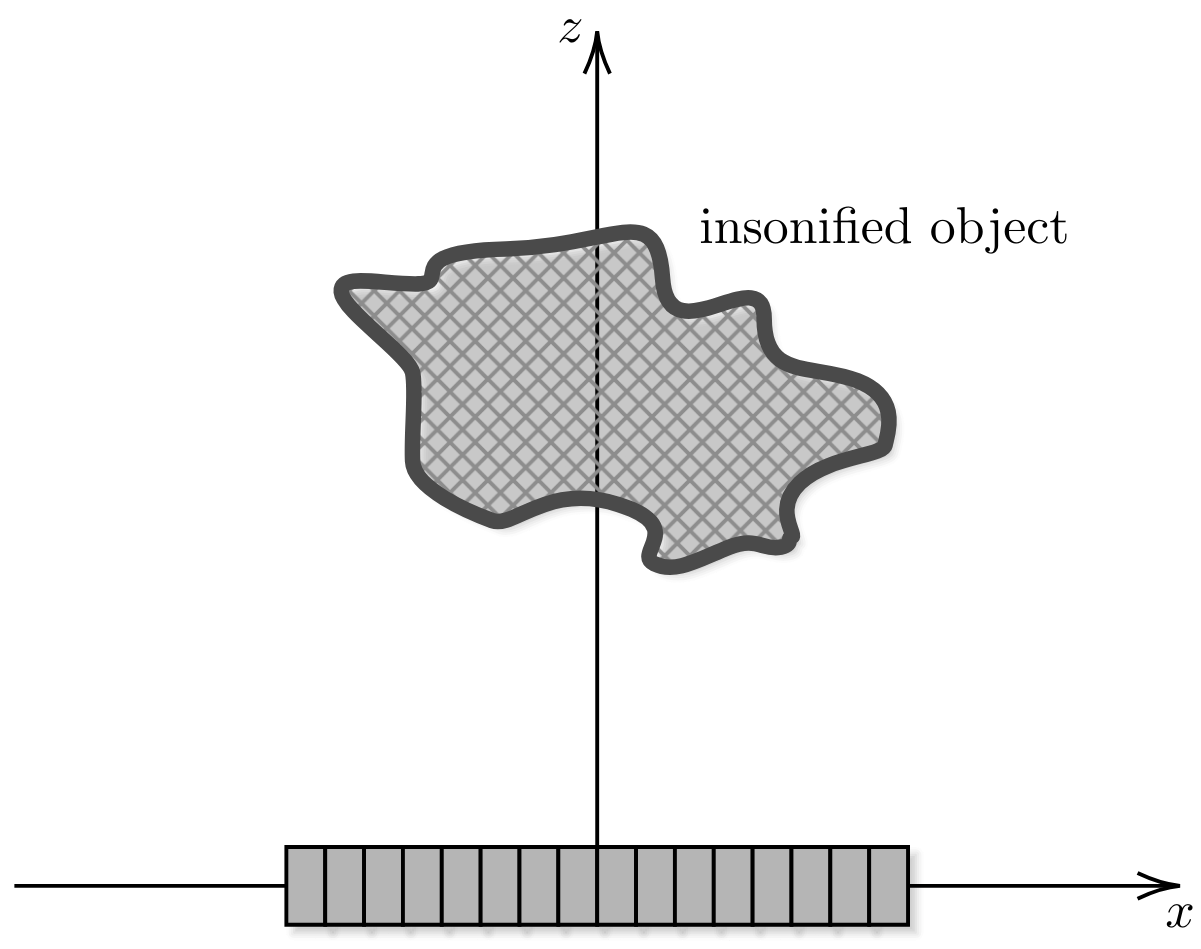
\includegraphics[width=0.5\textwidth]{images/array.png}
    \captionsetup{justification=centering}
    \caption{Sender/receiver array for ultrasound imaging \cite{Dorausch_2022}}
    \label{fig:us_array}
\end{figure}

The algorithm used for this k-space analysis is the \ac{fbi} proposed by Dorausch et al. This paper consists of three main parts the Fourier transformation into the k-space, the reconstruction of the image with the transformed data and the back transformation to get the final image. As it is important for an clinical ultrasound device the algorithm was investigated for its real time capability. In his bachelor thesis Richter \cite{Richter_2024} compared the implementation of this algorithm on different hardware. Once on a \ac{cpu} and once of the \ac{gpu} of a Snapdragon processor. For the analysis on an mobile processor synthetic data for 16 sender and 128 receiver was used. In figure \ref{fig:fft_an} it is shown that the \ac{fft} exceeds the realtime goal of 30 ms for a steady video output by approximately 10 times even with the implementation on a \ac{gpu}. It becomes clear that the \ac{fft} is the bottleneck for a realtime implementation of the image reconstruction algorithm. Therefore an efficient implementation of a large \ac{fft} is needed. The requirements for such an algorithm are discussed in the next chapter\cite{Dorausch_2022}.

\section{Realtime requirements} \label{sec:req}
As the algorithm proposed in this work should contribute to an image with the maximum possible quality some of the requirements are higher than in previous work. The goal of this thesis is to enable the realtime capability of an \ac{fft} algoritm for a system with 256 receivers and 10 senders. A property of the \ac{fbi} algorithm is that the use of longer signals leads to better imaging results. A sufficient length for this signal is 4 ms \cite{dorausch_adoption_2023}. Each of the 256 receivers records the reflection of this signal. The analogue signal is then sampled with an \ac{adc} with a sampling rate of 65.536 MHz and a resolution of 16 bit for one datapoint. This results in a $2^{18}$ datapoint \ac{fft} with 16 bit datapoints for every receiver. If again 30 ms goal for a steady 30 frames per second video stream is assumed, this means that 256 $2^{18}$ \ac{fft}s need to be done within 30 ms.

\begin{figure}[h!]
    \centering
    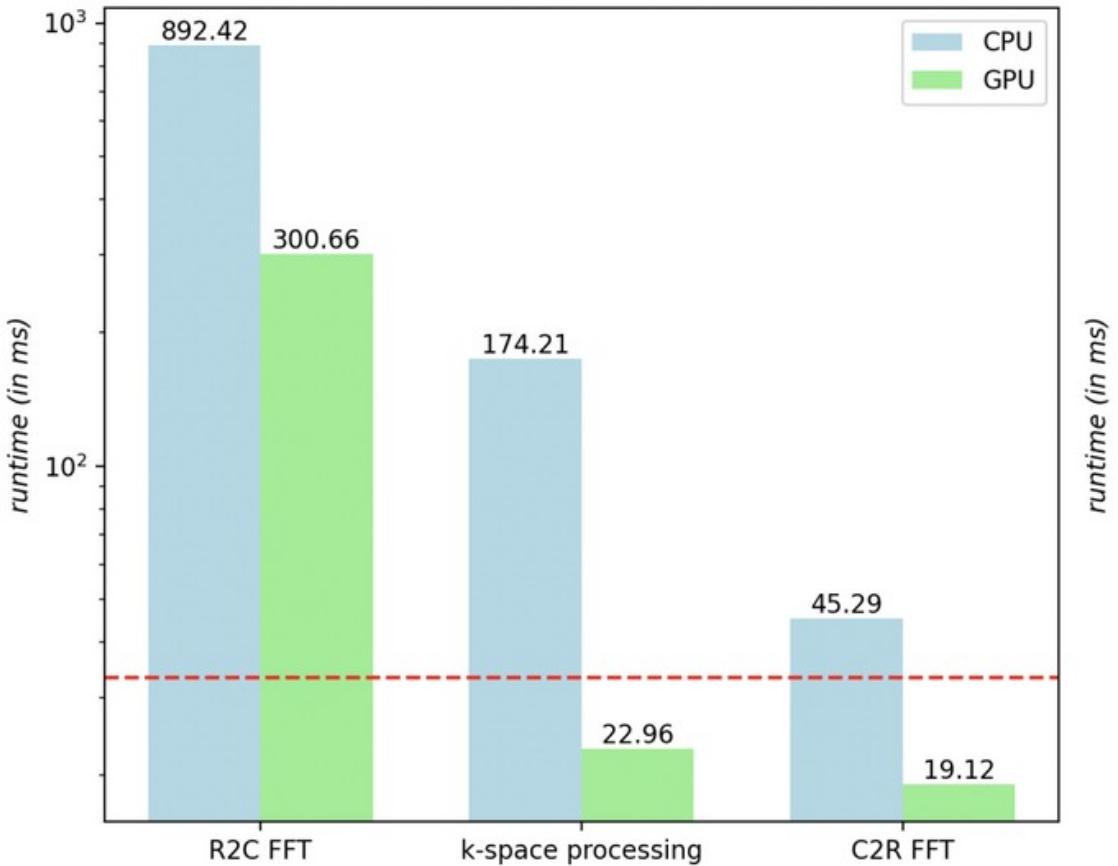
\includegraphics[width=0.4\textwidth]{images/fft_an.png}
    \captionsetup{justification=centering}
    \caption{Different parts of the \ac{fbi} algorithm by runtime and hardware \cite{Richter_2024} }
    \label{fig:fft_an}
\end{figure}

\section{Fast Fourier Transform}\label{sec:ft}
The Fourier transform is a foundational tool in digital signal processing, essential for analyzing the frequency components of signals. Fundamentally, it decomposes a signal into a set of sinusoids, each with a unique frequency, amplitude, and phase. This decomposition is typically implemented via the \ac{dft} or its efficient computation, the \ac{fft}. Equation \ref{eq:fft} shows the \ac{dft} \cite{muller_fundamentals_2015}.\par

\begin{equation}\label{eq:dft}
    X(k) = \sum_{n=0}^{N} x(n) e^{\frac{-2\pi i k n}{N}}\
\end{equation}

For real-time capability of the Discrete Fourier Transform, not only in Fourier-based imaging but 
also in other scenarios, fast computation is essential. One of the most renowned algorithms for 
achieving this is the Cooley-Tukey \ac{fft} algorithm. This algorithm significantly reduces the computational complexity 
of the \ac{dft} from \(O(n^2)\) to \(O(n \log n)\) using a divide-and-conquer approach, where the 
problem size is reduced for each computation. The main concept behind the Cooley-Tukey algorithm 
is to reduce the computational complexity of the \ac{dft} by exploiting symmetries and factoring the \ac{dft} 
into smaller components, which significantly decreases the number of operations needed. 
This design also allows for parallel computation, as not all operations depend on one 
another anymore \cite{cooley_algorithm_1965}.\par
To understand the construction of the Cooley-Tukey algorithm, it's best to begin with the radix-2 
case. The name stems from decomposing a \ac{dft} of length \(N\) into two interleaved \ac{dft}s with sizes 
\(N/2\). The initial step of this decomposition involves splitting the \ac{dft}, as defined in 
equation \ref{eq:dft}, into a sum of the even-indexed parts and the odd-indexed parts for 
\(k = N/2 - 1\).

\begin{equation}\label{eq:dft_even_odd}
    X(k) = \sum_{m=0}^{N/2 - 1} x(2m) e^{\frac{-2\pi i}{N} (2m) k} + \sum_{m=0}^{N/2 - 1} x(2m+1) 
    e^{\frac{-2\pi i}{N} (2m+1) k}\
\end{equation}

The multiplier \(e^{\frac{-2\pi i k}{N}}\) can be factored out, as shown in equation 
\ref{eq:even_odd_e}. This representation makes it clearer that the first \(N/2\) entries of the 
\ac{dft} are obtained by computing the \ac{dft} over the even-indexed parts and the \ac{dft} over the odd-
indexed parts separately. These results are then combined into an output vector, where the odd-
indexed parts are adjusted by the factors \(e^{\frac{-2\pi i k}{N}}\), known as the twiddle 
factors \cite{duhamel_fast_1990}.

\begin{equation}\label{eq:even_odd_e}
    X(k) = \sum_{m=0}^{N/2 - 1} x(2m) e^{\frac{-2\pi i}{N/2} mk} + e^{\frac{-2\pi i k}{N}} 
    \sum_{m=0}^{N/2 - 1} x(2m+1) e^{\frac{-2\pi i}{N/2} mk}\
\end{equation}

The calculation for the second \(N/2\) entries follows a similar pattern, as shown in equation 
\ref{eq:second_m}. The key distinction lies in the common multiplier factored out, which is 
\(e^{\frac{-2\pi i}{N}  (k + \frac{N}{2})}\). Due to the periodicity of \(e\), this is equivalent 
to \(-e^{\frac{-2\pi i k}{N}}\), as illustrated in equation \ref{eq:second_m_s}.

\begin{equation}\label{eq:second_m}
    X(k + \frac{N}{2}) = \sum_{m=0}^{N/2 - 1} x(2m) e^{\frac{-2\pi i}{N} (2m) (k + \frac{N}{2})} + 
    \sum_{m=0}^{N/2 - 1} x(2m+1) e^{\frac{-2\pi i}{N} (2m+1) (k + \frac{N}{2})}\
\end{equation}

\begin{equation}\label{eq:second_m_s}
    X(k + \frac{N}{2}) = \sum_{m=0}^{N/2 - 1} x(2m) e^{\frac{-2\pi i}{N/2} mk} - e^{\frac{-2\pi i 
    k}{N}} \sum_{m=0}^{N/2 - 1} x(2m+1) e^{\frac{-2\pi i}{N/2} mk}\
\end{equation}

Designating the even indexed \ac{dft} as \(E_{k}\) and the odd indexed \ac{dft} as \(O_{k}\), the entire \ac{dft} 
can be expressed in the form of the following two equations:

\begin{equation}\label{eq:even_dft}
    X(k) = E_{k} + e^{\frac{-2\pi i k}{N}} O_{k}\
\end{equation}

\begin{equation}\label{eq:odd_dft}
    X(k + \frac{N}{2}) = E_{k} - e^{\frac{-2\pi i k}{N}} O_{k}\
\end{equation}

In these equations, the final results are obtained by combining the two \ac{dft}s \(E_{k}\) and 
\(O_{k}\) through a +/- operation. This addition for the even parts and subtraction for the uneven parts, 
commonly referred to as a butterfly, is itself a \ac{dft}. With this understanding, a more general form of the 
\ac{fft} algorithm can be derived, where the butterfly operation is not limited to inputs of two. Instead, 
larger \ac{dft}s can be used to combine the results, with the size often referred to as the radix, describing 
the resulting combining \ac{dft} \cite{muller_fundamentals_2015}.\par
This implies that a large \ac{dft} of size \(N\) can be decomposed into two smaller \ac{dft}s of sizes 
\(N_{1}\) and \(N_{2}\), where \(N = N_{1} * N_{2}\). In this scenario, \(N_{1}\) \ac{dft}s of size 
\(N_{2}\) would be performed first. The results of this stage would then be combined with 
\(N_{2}\) \ac{dft}s of size \(N_{1}\). This generalization can be expressed in the following equation:

\begin{equation}\label{eq:fft}
    X(k) = \sum_{n_{1} = 0}^{N_{1} - 1} e^{\frac{-2\pi i}{N_{1} N_{2}}n_{1}k_{2}} (\sum_{n_{2} = 0}
    ^{N_{2} - 1} x_{N_{1}n_{2}+n_{1}} e^{\frac{-2\pi i}{N_{2}}n_{2}k_{2}}) e^{\frac{-2\pi i}{N_{1}}
    n_{1}k_{1}}
\end{equation}


One crucial aspect of this algorithm is its potential for recursive application. All smaller \ac{dft}s 
can be addressed by the Cooley-Tukey algorithm itself and decomposed into even smaller \ac{dft}s. This 
recursive approach leads to the notion that a decomposition is the radix \(X\) of an \ac{fft}, meaning 
that all \ac{dft}s larger than \(X\) are successively reduced until they reach the size of \(X\).\par
Moreover, it is feasible to employ mixed radix decomposition, incorporating different radices at 
various stages of the \ac{fft}. This results in multiple possible decompositions of a single \ac{dft} 
\cite{qureshi_generation_2011}. The primary differences between these variants lie in the level of 
parallel transforms and the complexity of the twiddle factors. This complexity can be 
advantageous, as periodicity of the twiddle factors can lead to simplifications. While many of 
these simplifications may not be of significant mathematical interest, they play a crucial role in 
hardware implementation. Determining which simplifications are essential depends on understanding 
the underlying hardware. Consequently, the next section will provide an overview of the hardware 
utilized in this thesis.
%TODO one paragraph for comparison with \ac{dft}2d


%TODO adopt this whole section
\section{Versal Adaptive Computer Acceleration Platform}\label{sec:versal}
The hardware basis for this thesis is the VCK190 evaluation board with the VC1902 Adaptive Computer 
Acceleration Platform (ACAP), developed by Xilinx. The ACAP is a heterogeneous \ac{soc}
comprising multiple integrated hardware components and user-programmable hardware designs. All of these 
components are interconnected via a \ac{noc}. The network employs an AXI4 network, 
implemented outside the configurable logic blocks, which frees up resources. The hardware components 
dedicated to computing can be divided into three main categories. As illustrated in figure 
\ref{fig:high_scheme}, the aforementioned main components can be classified into three categories: 
scalar engines, adaptable engines and intelligent engines \cite{AMD_a_aie}.\par

\begin{figure}[h]
    \centering
    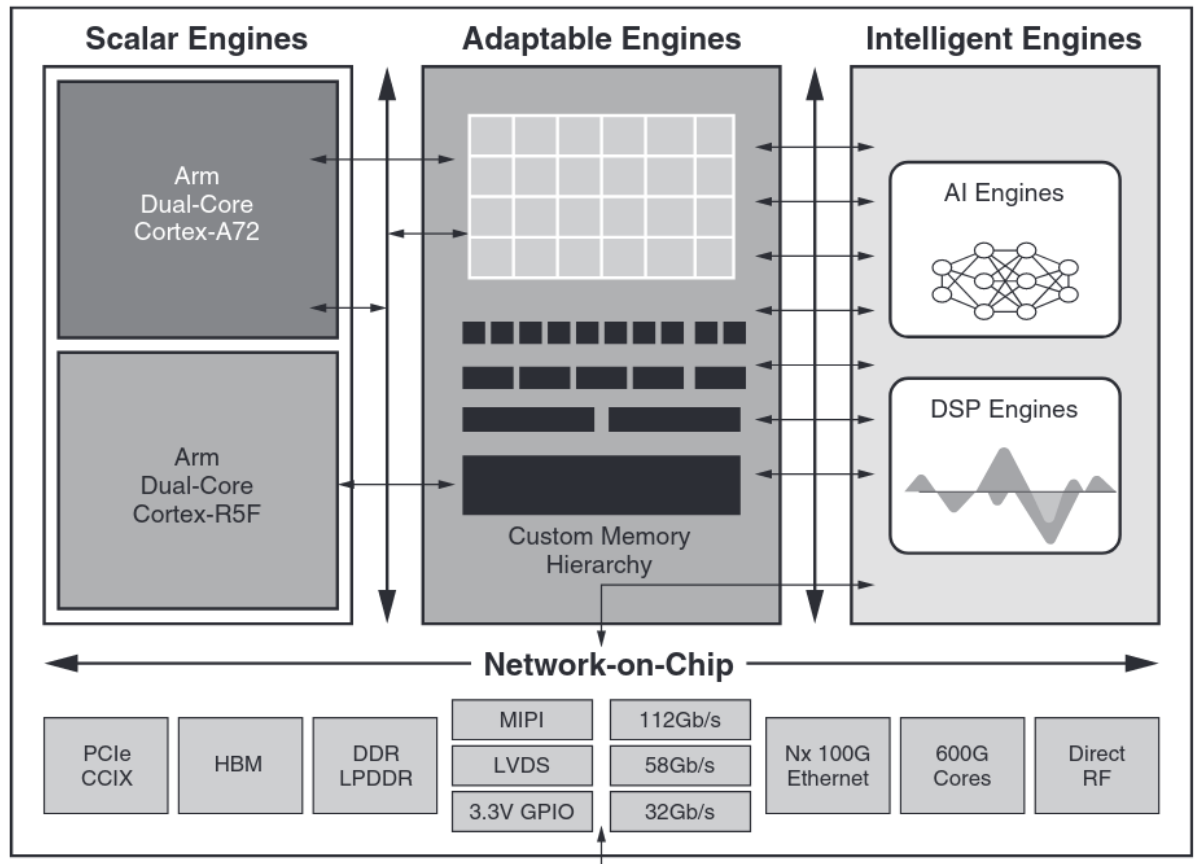
\includegraphics[width=0.6\textwidth]{images/high_level_vc1902.png} %adopt font and textsize
    \captionsetup{justification=centering}
    \caption{Overview of the VC1902 \cite{AMD_a_aie}}
            Highlevel view of the VC1902 which shows the three main parts which are connected via a \ac{noc}. Shows also some of the peripheral elements like Ethernet and memory controller
    \label{fig:high_scheme}
\end{figure}

\subsection{Scalar Engines}
The scalar engines are composed of the ARM-Cortex-A72 CPU and an ARM-Cortex-R5F real-time CPU. In 
conjunction with peripheral components, including USB, UART and PCIe controllers, they constitute the 
processing system (PS). This system is connected to the DDR memory controller via the \ac{noc}, which allows 
the sharing of this controller with the \ac{pl}. In an embedded system, the primary 
function of the processing system is to serve as a host for other system components. The software is 
executed and specific hardware-optimised components are delegated to the adaptable engines or 
intelligent engines. The ARM cores permit either the execution of bare-metal applications for this 
scenario or the hosting of a full operating system, which allows the user to take advantage of the 
system's features and usermode libraries for interaction with the \ac{pl}. In this work, the 
latter case is employed with the Petalinux operating system, developed by Xilinx for their boards. This 
enables the use of the Xilinx runtime environment (XRT) to interact with the adaptable engines and 
intelligent engines, thereby facilitating the utilisation of special libraries to reduce the 
development overhead associated with existing software and hardware features \cite{AMD_a_aie}.

\subsection{Adaptable Engines}
The term "programmable logic" is used to describe the adaptable engines. The system comprises 
configurable logic blocks (CLBs), internal memory, and digital signal processing (DSP) engines. It can 
be considered an \ac{fpga} like structure that enables the processing of irregular data. The CLBs utilise 
the conventional design of look-up tables (LUTs) and flip-flops. The internal memory of the \ac{pl} 
comprises 967 block-RAM elements, each of which can store 36 kilobytes of data, and 463 ultra-RAM 
elements, which can hold 288 kilobytes of memory each. To enhance flexibility, the \ac{pl} is partitioned 
into multiple clock regions. Typically, such regions contain 24 block and ultra-RAM elements. In order 
to transfer data between \ac{pl} endpoints, the \ac{noc} is employed. This is typically done via the PS or other 
integrated blocks. The NoC can be employed to free resources in the \ac{pl} that would otherwise be used for 
routing, thus facilitating communication between different \ac{pl} endpoints. The connection to the NoC can 
be configured with AXI3, AXI4, or AXI4 Stream. The NoC employs a 128-bit-wide NoC packet protocol 
internally \cite{AMD_a_aie}.\par

\begin{figure}[h]
    \centering
    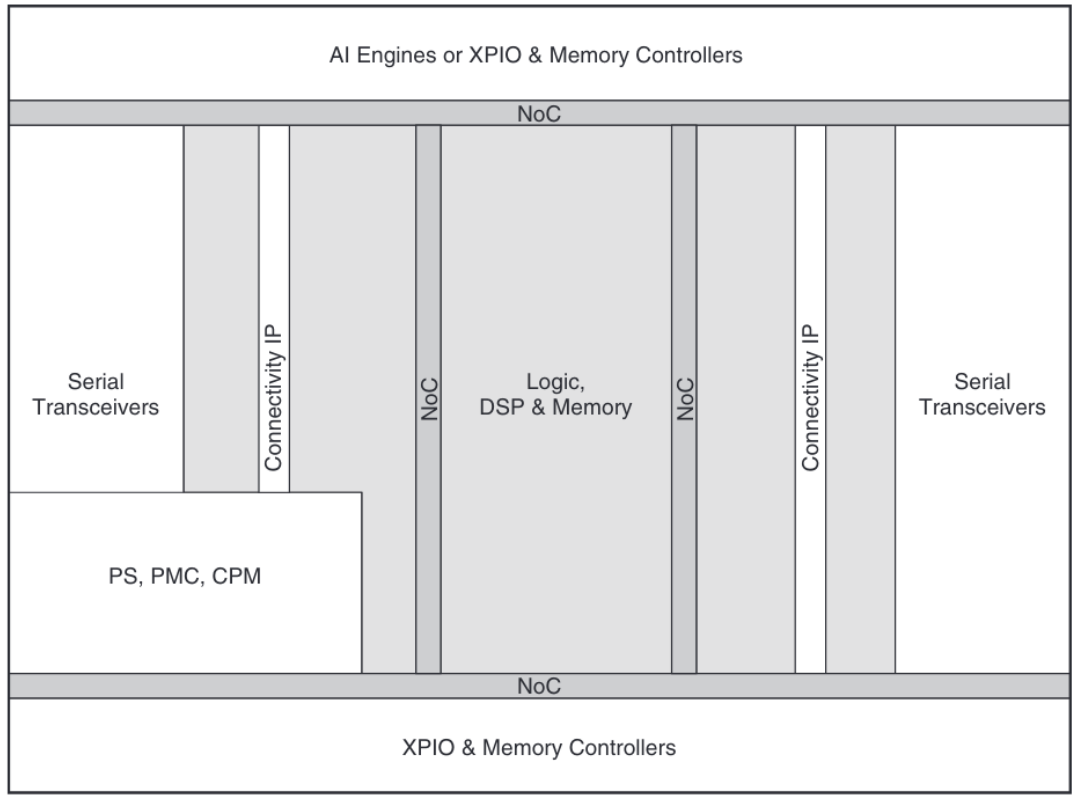
\includegraphics[width=0.6\textwidth]{images/low_level_vc1902.png}
    \captionsetup{justification=centering}
    \caption{Schematic of the VC1902 chip design \cite{AMD_a_aie}}
            Deeper look into the organisation of the three main components. It is shown that this elements are much more integrated than shown in previous schematics. 
    \label{fig:low_scheme}
\end{figure}

\subsection{Intelligent Engines}
The intelligent engines comprise digital signal processors (DSP) elements and artificial intelligence 
(AI) engines. The DSP elements are not formally part of the intelligent engines. As illustrated in 
figure \ref{fig:low_scheme}, the DSP elements are situated within the \ac{pl}. This is due 
to the structure of such an DSP element, which consists of a 27-bit pre-adder, a 27x28 multiplier, and 
a 48-bit arithmetic logic unit (ALU), as illustrated in figure \ref{fig:dsp}. Additionally, it 
comprises a multitude of registers for the storage of input values and results. In order to optimise 
the utilisation of these elements, it is necessary to employ the use of memory, such as block RAM, 
which must be directly connected to the element in question. Another crucial aspect of placing these 
elements in a \ac{pl} is the capability to cascade operations through multiple DSP elements. 
This is made possible through the CARRYCASCIN and CARRYCASCOUT pins. Furthermore, single instruction 
multiple data (SIMD) operations are made available. In conjunction with cascading two 24-bit SIMD 
accumulators or four 12-bit SIMD accumulators, the aforementioned elements can be employed. 
Furthermore, the internal MULTSIGNIN and MULTSIGNOUT cascade signals permit the utilisation of 96-bit 
multiply-accumulate (MAC) operations \cite{AMD_a_aie}.\par

\begin{figure}
    \centering
    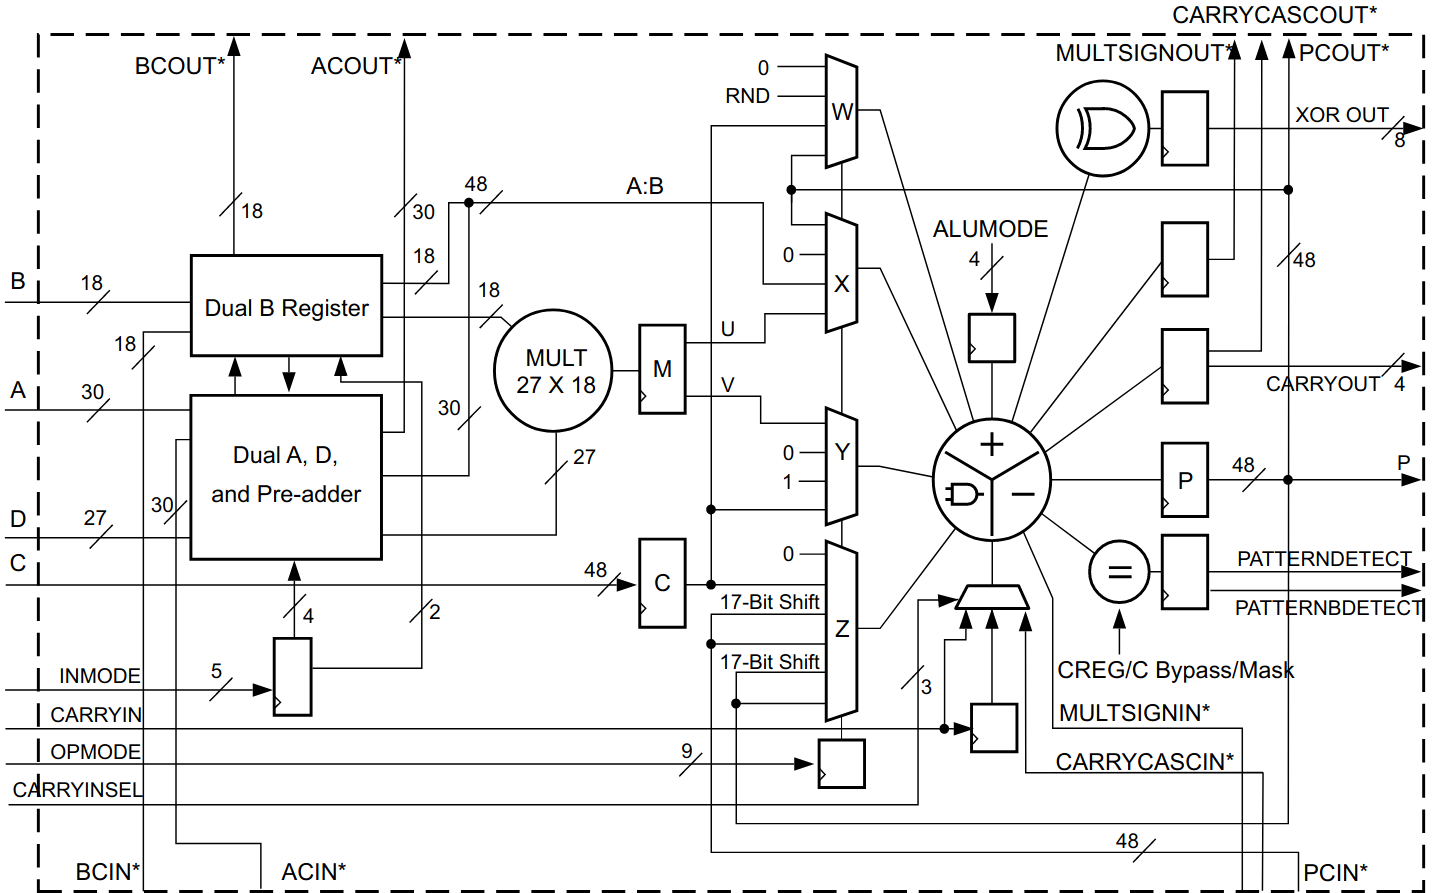
\includegraphics[width=0.7\textwidth]{images/dsp_detail.png}
    \captionsetup{justification=centering}
    \caption{Detailed schematic of the DSP Slice \cite{AMD_a_aie}}
            The interconnection between multiplexer, adder and multiplication units within the DSP is shown. Additional single bit lane are highlighted to show potential cascade connections.
    \label{fig:dsp}
\end{figure}

\subsubsection{AI Engines}
Another essential component of the intelligent engines is the AI Engine array, comprising newly developed AI accelerators, as previously mentioned. The VCK190 platform includes 400 of these engines, arranged in a two-dimensional tile array. This array is connected to \ac{pl} through eight specialized connection tiles, supporting the AXI standard \cite{AMD_a_aie}.\par

\begin{figure}[h!]
    \centering
    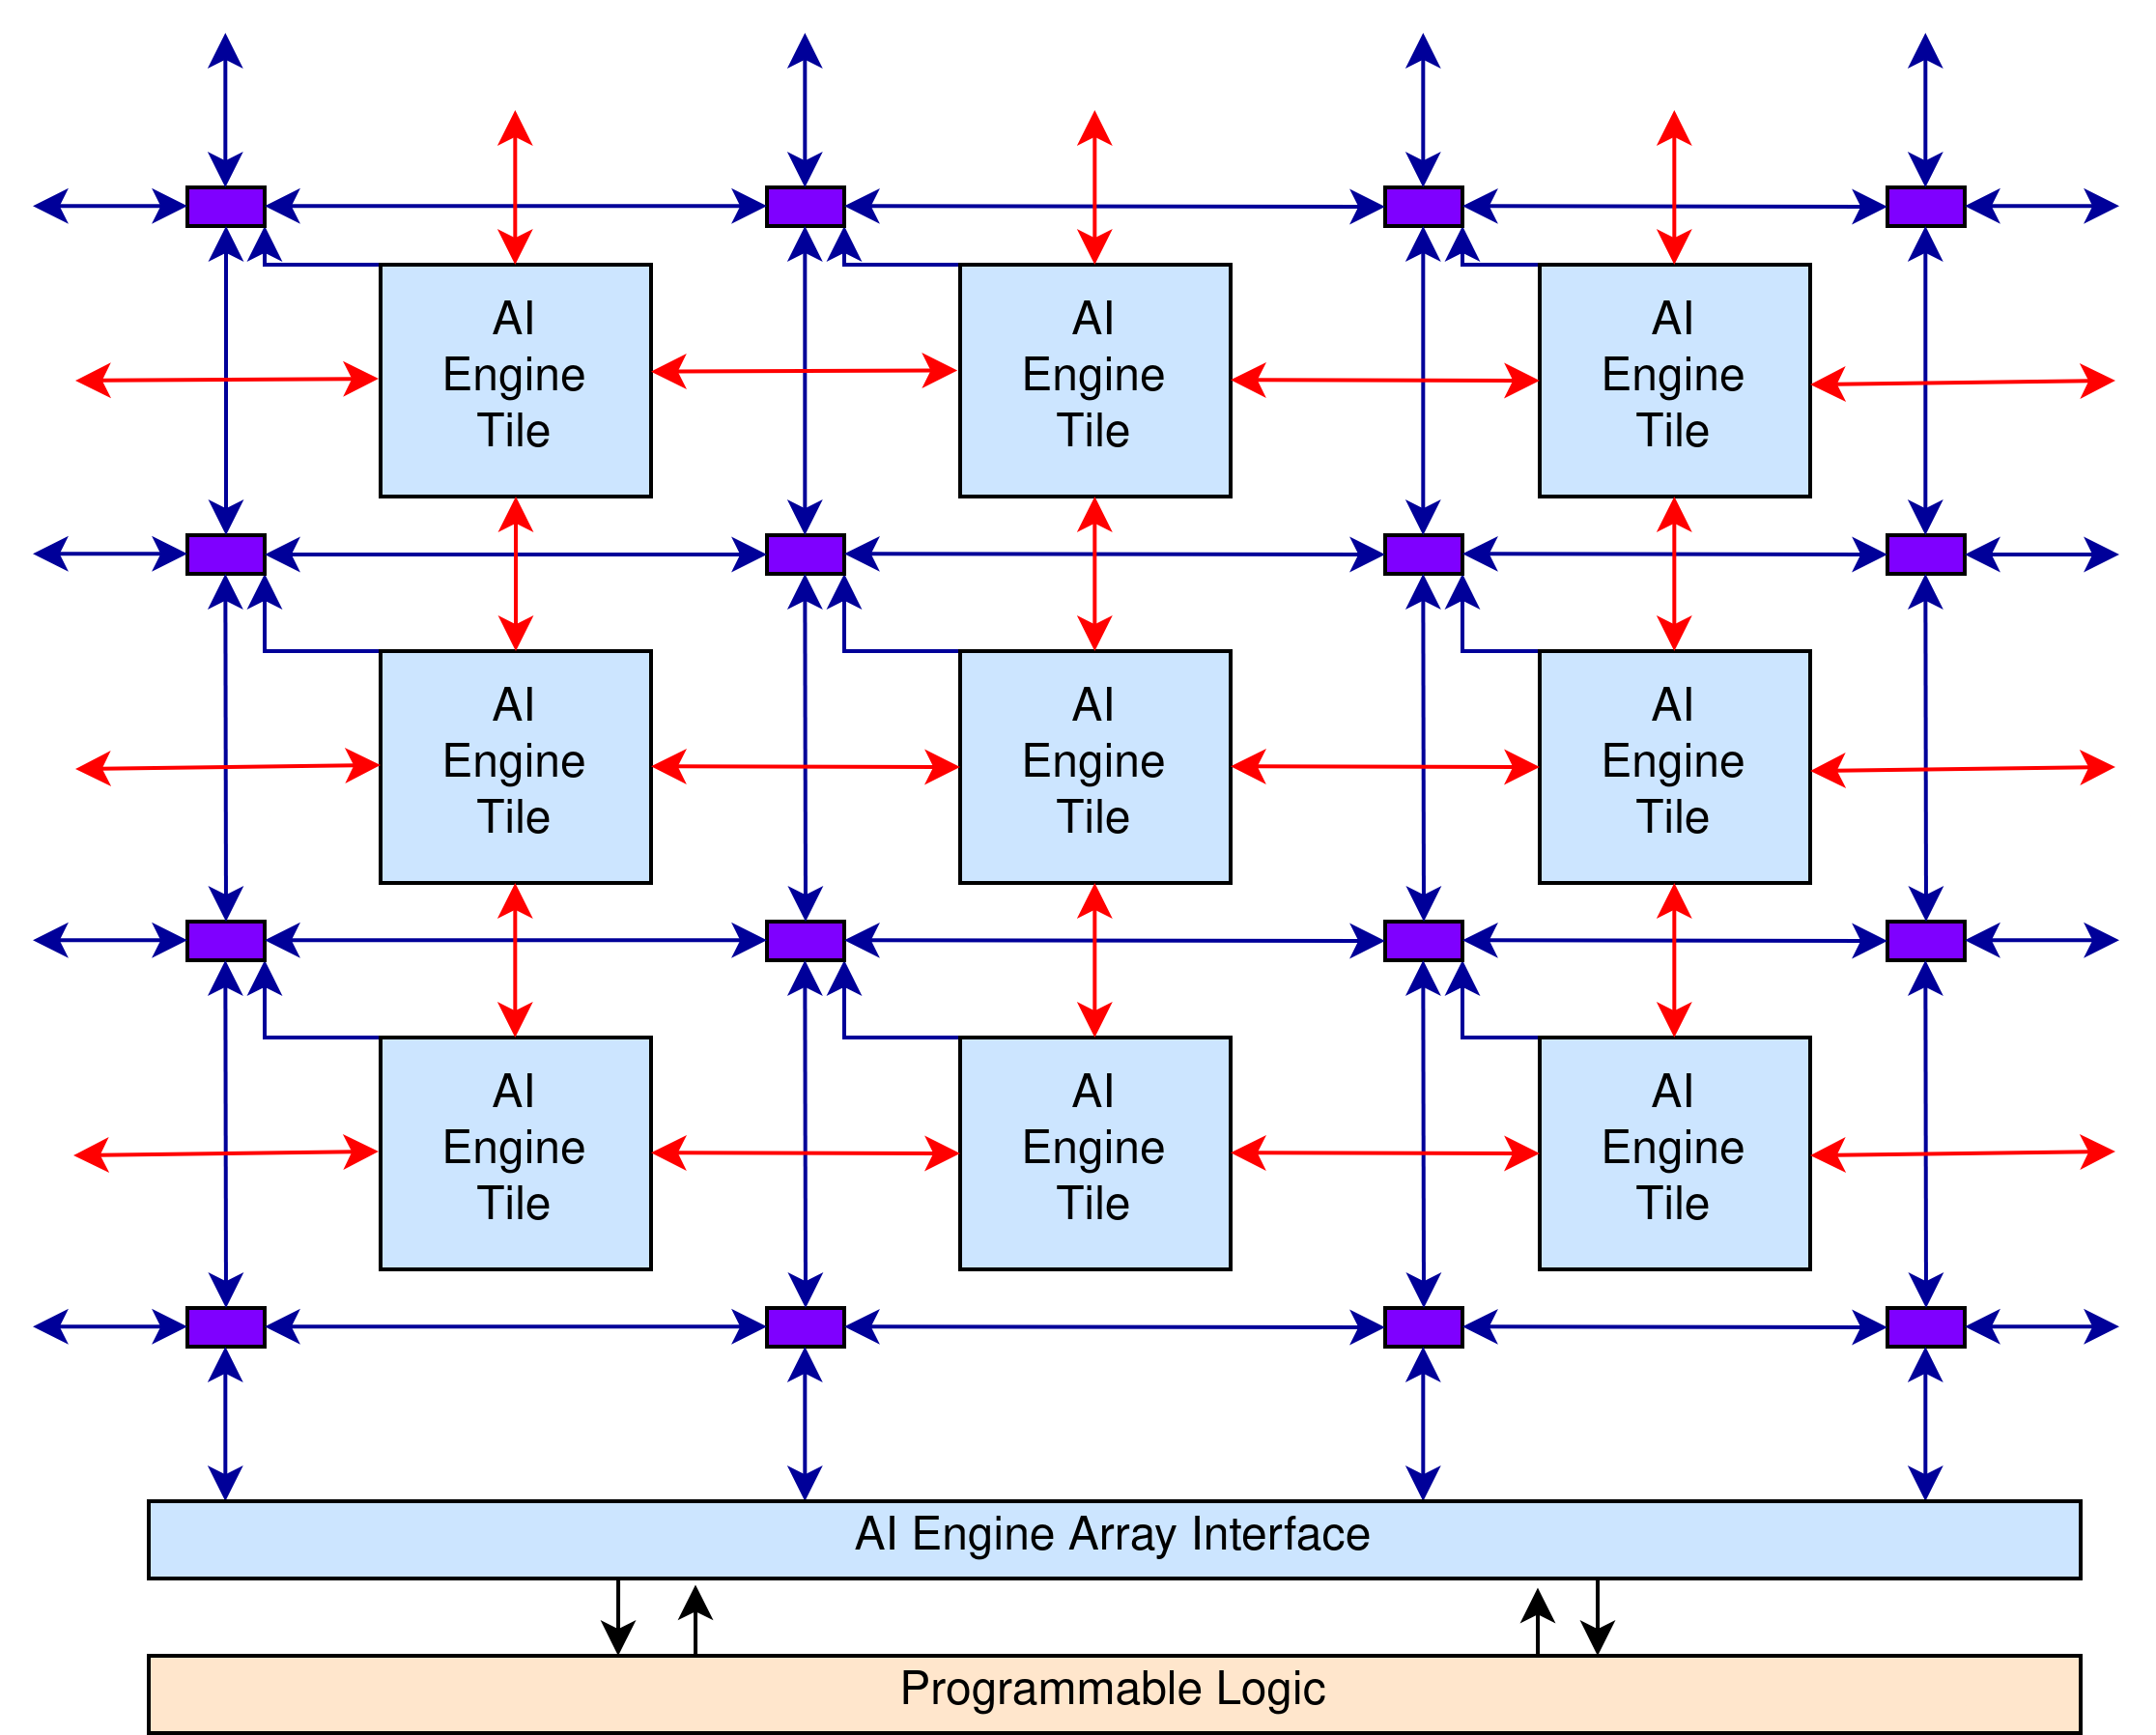
\includegraphics[width=0.7\textwidth]{images/ai_array.png}
    \captionsetup{justification=centering}
    \caption{AI Engine array}
            A schematic that shows the AI Engine array with its different connections. Red connections between the tiles show the direct memory access between tiles while purple shows the streaming interface between further away tiles. At the bottom of the array the interface to the PL is shown \cite{AMD_a_aie}.
    \label{fig:ai_array}
\end{figure}

As depicted in figure \ref{fig:ai_array}, each tile in the array is interconnected, featuring two primary types of communication pathways. The first is an AXI-based network connecting all tiles. This network facilitates data transmission among the tiles via a routing and switching system that can split or merge multiple data streams. Specifically, the network can divide a single stream into up to 32 sub-streams or merge up to 32 sub-streams back into a single stream. This stream management is enabled by data packet headers, which identify the respective substream for routing.\par
The second type of connection provides direct access between adjacent tiles, where each tile can access the memory of its neighboring tiles to the north, south, east, and west. This arrangement allows for efficient memory usage and reduces memory overhead, particularly when two accelerators require shared memory access.\par
To provide a deeper understanding of this technology, the specific structure of the tiles is outlined in detail. As illustrated in figure \ref{fig:detail_tile}, each tile contains the aforementioned memory and an AI Engine core, which serves as the primary accelerator. This memory comprises 32 KB, divided into eight 8 KB banks, each accessible in parallel by the streaming interfaces. As noted earlier, this memory can also be accessed by neighboring AI Engine cores on adjacent tiles \cite{AMD_aie_k}.\par

\begin{figure}[h!]
    \centering
    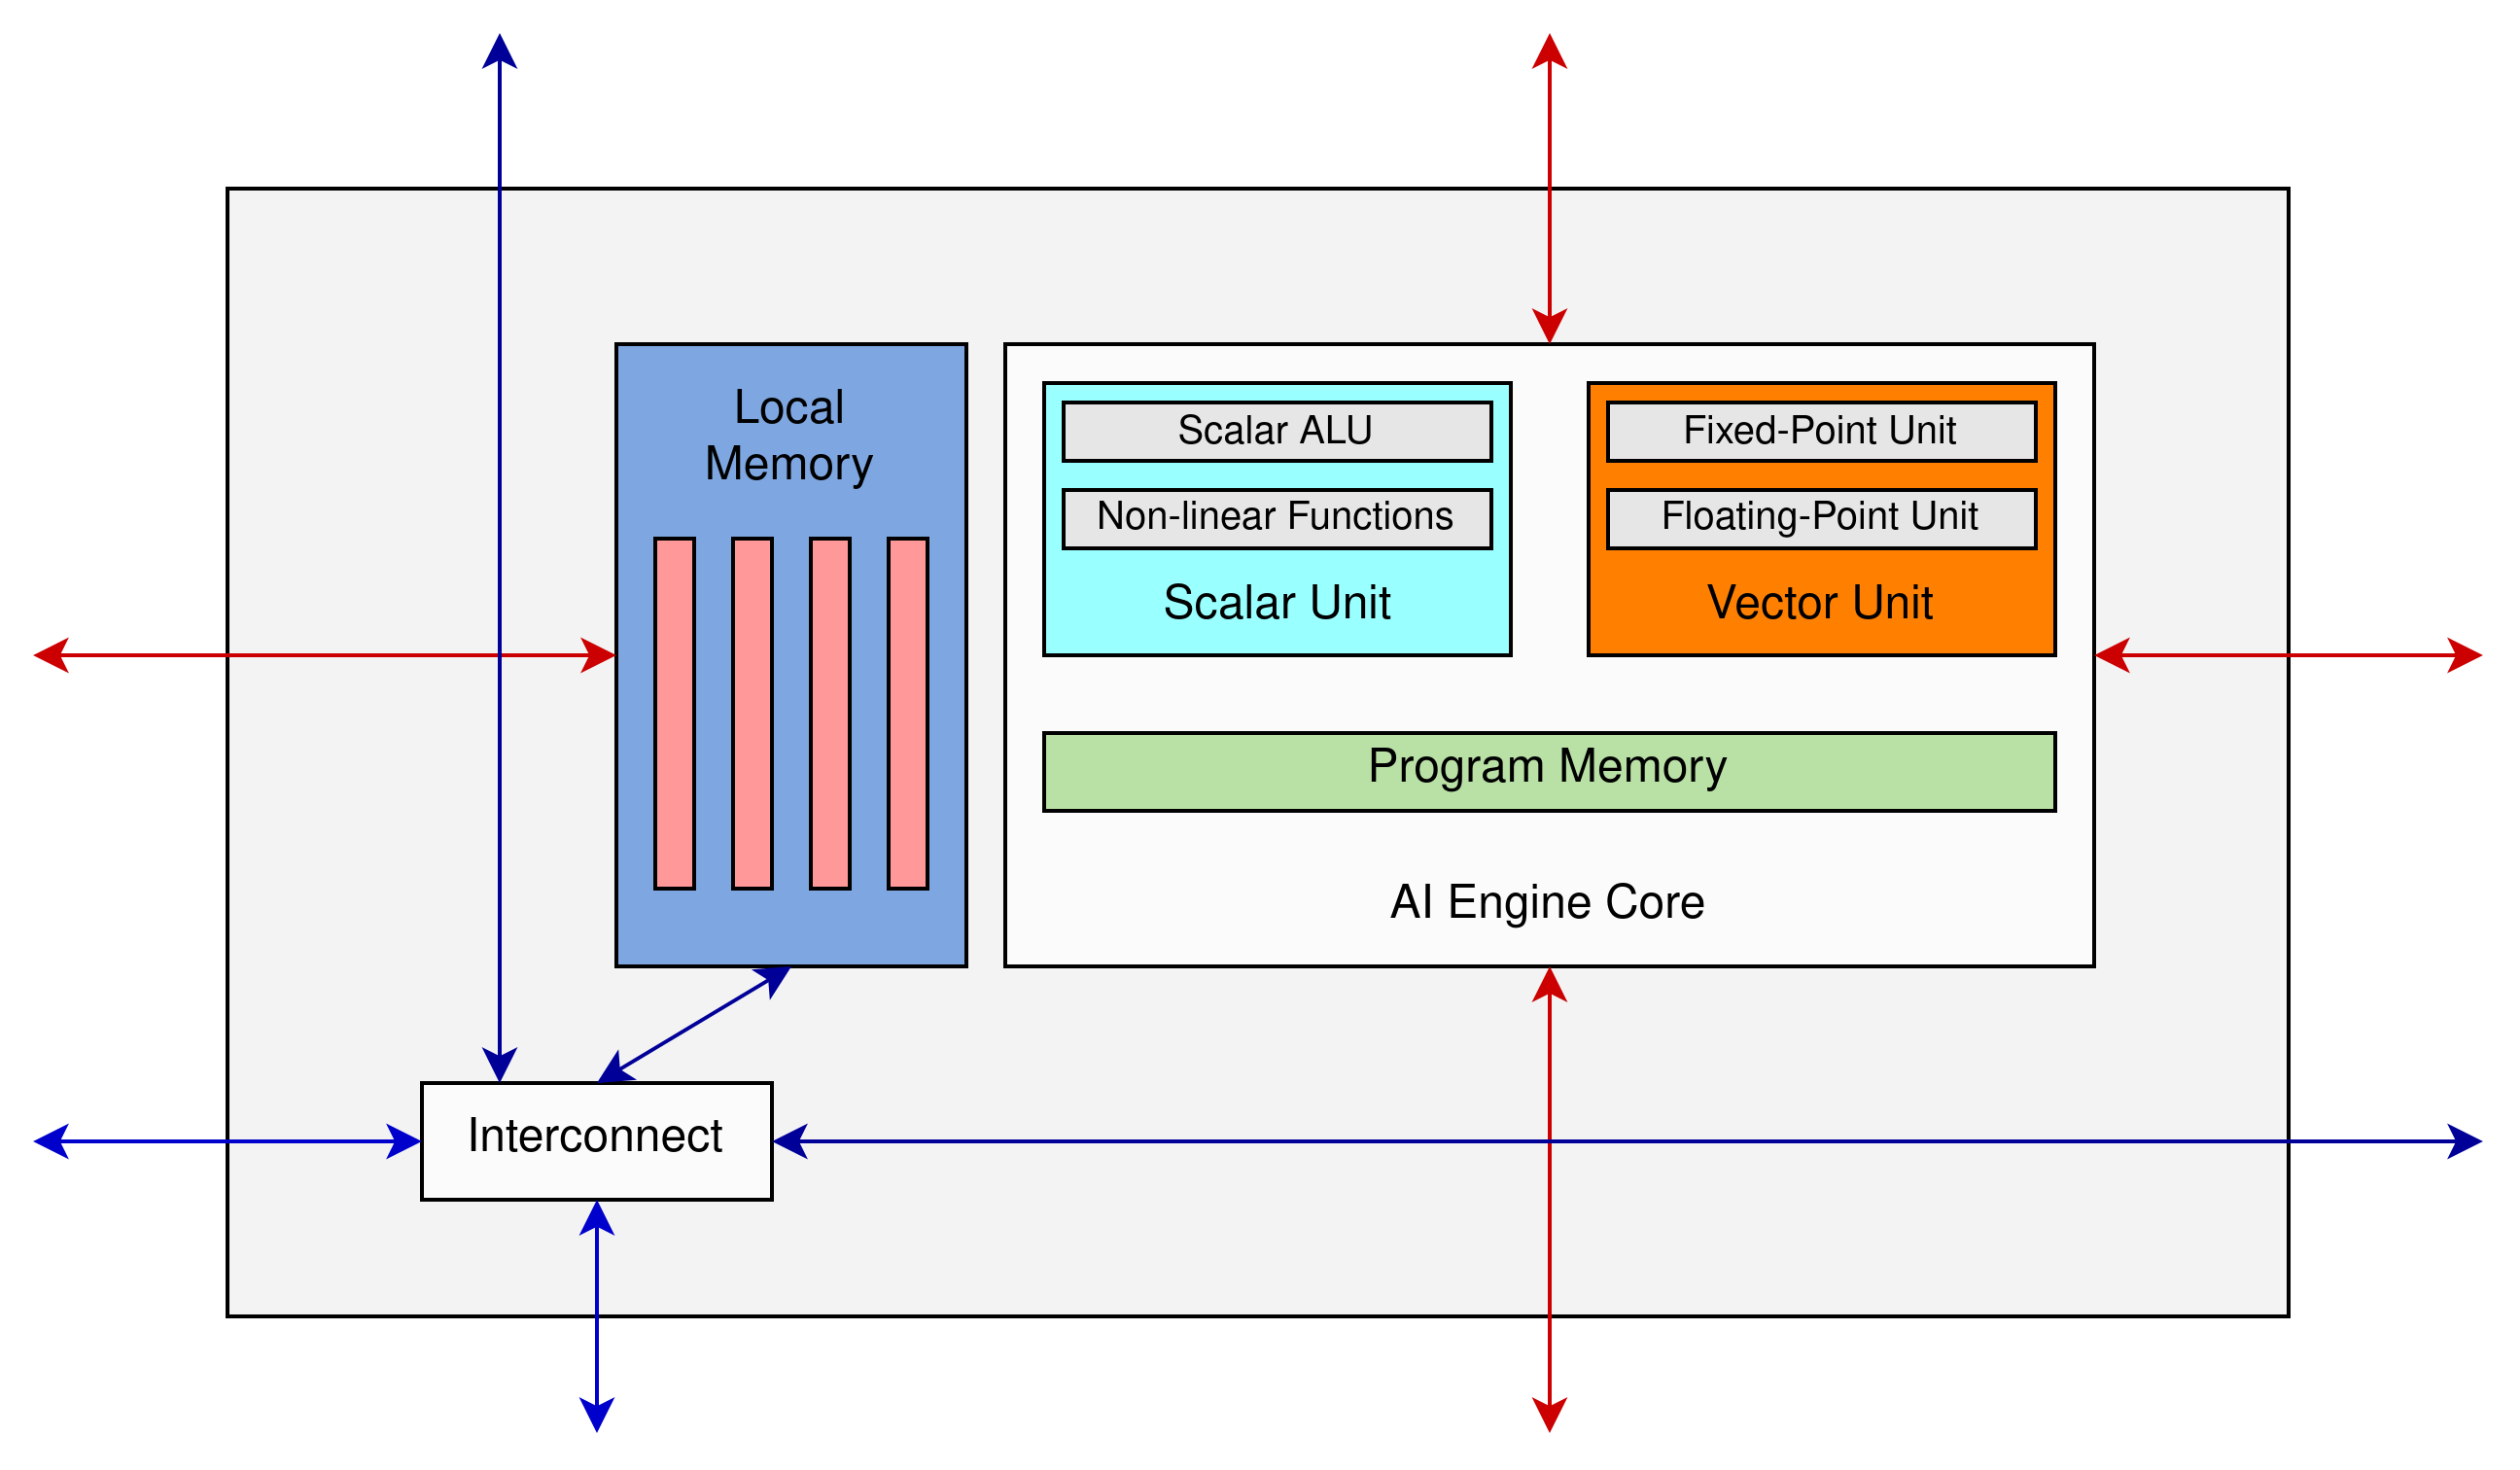
\includegraphics[width=0.9\textwidth]{images/detail_tile.png}
    \captionsetup{justification=centering}
    \caption{AI Engine tile}
            Detailed look into the AI Engines with the different component of the core. The four local memory banks of the core are shown in red, the different calculation units of the RISC processor are shown in blue (scalar) and orange (vector). Connections to the other tiles within the array are also highlighted. 
    \label{fig:detail_tile}
\end{figure}

The AI Engine core itself is a compact \ac{risc} processor equipped with 16 KB of dedicated program memory, as well as one scalar and one vector processing unit. The vector unit's register structure is depicted in the table \ref{tab:reg}. At the hardware level, the vector unit includes 16 registers, each 128 bits wide, which can be combined to form larger registers as needed. These registers can be addressed directly via a dedicated storage directive, utilizing the register names specified in the figure. This registers can be accessed with special functions so called intrinsics . They allow fine grained access to this registers and enable to full use of the vector unit \cite{AMD_aie_intrinsics, AMD_a_aie_s}.\par

\begin{table}
\centering
\resizebox{0.4\textwidth}{!}{
\begin{tblr}{
  cells = {c},
  cell{1}{4} = {c=2}{},
  cell{2}{2} = {r=2}{},
  cell{2}{3} = {r=4}{},
  cell{2}{4} = {r=8}{},
  cell{2}{5} = {r=4}{},
  cell{4}{2} = {r=2}{},
  cell{6}{2} = {r=2}{},
  cell{6}{3} = {r=4}{},
  cell{6}{5} = {r=4}{},
  cell{8}{2} = {r=2}{},
  cell{10}{2} = {r=2}{},
  cell{10}{3} = {r=4}{},
  cell{10}{4} = {r=4}{},
  cell{10}{5} = {r=4}{},
  cell{12}{2} = {r=2}{},
  cell{14}{2} = {r=2}{},
  cell{14}{3} = {r=4}{},
  cell{14}{4} = {r=4}{},
  cell{14}{5} = {r=4}{},
  cell{16}{2} = {r=2}{},
  vlines,
  hline{1-2,10,14,18} = {-}{},
  hline{3,5,7,9,11,13,15,17} = {1}{},
  hline{4,8,12,16} = {1-2}{},
  hline{6} = {1-3,5}{},
}
128-bit & 256-bit & 512-bit & 1024-bit &              \\
vrl0    & wr0     & xa      & ya       & N/A          \\
vrh0    &         &         &          &              \\
vrl1    & wr1     &         &          &              \\
vrh1    &         &         &          &              \\
vrl2    & wr2     & xb      &          & {yd\\(msbs)} \\
vrh2    &         &         &          &              \\
vrl3    & wr3     &         &          &              \\
vrh3    &         &         &          &              \\
vcl0    & wc0     & xc      & N/A      & N/A          \\
vch0    &         &         &          &              \\
vcl1    & wc1     &         &          &              \\
vch1    &         &         &          &              \\
vdl0    & wd0     & xd      & N/A      & {yd\\(lsbs)} \\
vdh0    &         &         &          &              \\
vdl1    & wd1     &         &          &              \\
vdh1    &         &         &          &              
\end{tblr}
}
\caption{Vector registers of the vector unit \cite{AMD_aie_intrinsics}}
        The addressing scheme for the vector registers. Each column shows a different addressing scheme for different data width of the registers.
\label{tab:reg}
\end{table}

The initialization of the AI engines occurs during boot-up, and configurations cannot be altered during runtime. The code designated for each engine is compiled and loaded into the 16 KB program memory. Data flow between engines is organized in a predefined graph, which establishes routing information across the network connecting individual tiles. This graph is also initialized during boot-up.\par
Following initialization, the AI engines are managed through either the Scalar Engines or \ac{pl} using a target offloading approach. Data is transferred into the AI engine array for processing, after which it exits via the connection tiles in an AXI stream format. The \ac{pl} then either processes this data directly or writes it to the chip’s DDR memory, signaling the ARM host processor for further handling. The entire array operates at a fixed clock rate of 1250 MHz.

\chapter{Related Work}
%It must be clear what is being worked on elsewhere. Especially the gaps of the others should be made clear. Why is your own work, your own approach important in order to advance the state of the art? This chapter is ignored by many readers (but not by the reviewer ;-), also later in publications "Related Work" is an important thing. (5-15 pages)
The efficient implementation of the Fourier Transform is by no means an unknown problem. Because many analysis in signal processing relies on it there are various approaches 
for implementations. Most of them come from the radar filed and deal with less antennas and with a smaller density in reflected waves. Therefore the amount of data points which are recorded are less than in the ultra sound setup of this work. These approaches still yield valuable insides into how to construct a fast and efficient \ac{fft}. Therefore this chapter will give an overview over the previous work and discuss some downsides for the use case of this work.

%TODO citation for this section
\section{Effectiveness of FFT Implementations on GPU}
One potential component for executing large \ac{fft}s is the \ac{gpu}. Designed specifically for processing vast amounts of data, \ac{gpu}s can perform identical operations across multiple data points in parallel. This parallelization greatly benefits \ac{fft} implementations. As previously mentioned, the Cooley-Tukey approach divides the \ac{dft} into smaller segments, which can be processed concurrently. The functionality of a \ac{gpu} in this context operates as follows: data to be processed is first copied into the \ac{gpu}’s memory, where multiple processing units execute the same calculation on distinct subsets of the data. Modern \ac{gpu}s, specialized for this purpose, contain up to tens of thousands of these processing units. To utilize them, the program must partition the data into subsets and define a kernel, the specific calculation, to be applied to each subset. Research indicates that using a \ac{gpu} can significantly boost performance compared to a \ac{cpu}, with complete radix-2 \ac{fft} decompositions showing up to a 30-fold improvement in runtime \cite{puchala_effectiveness_2015}.\par
The primary limitation for \ac{gpu}-based \ac{fft}s, however, lies not in computational power but in memory bandwidth constraints during data exchanges with the \ac{cpu} \cite{lloyd_fast_2008}. All data must be transferred to the \ac{gpu}’s memory before processing and then copied back into the main memory afterward to enable further computations. This memory transfer overhead becomes an issue because the \ac{fft} is only one step in a larger image reconstruction process. One approach to address this limitation is to perform the entire \ac{fbi} algorithm on the \ac{gpu}. This was attempted by Richter, although it was restricted to smaller datasets. This restriction is critical because current \ac{fft} implementations on \ac{gpu}s allow for two main approaches. In the first, a large \ac{fft} is computed, but results must be copied back to main memory for further processing \cite{cufft}. In the second, \ac{fft}s are embedded within a larger computation, eliminating the need for repetitive data transfers. However, this approach currently only supports \ac{fft} sizes up to 256 points \cite{cufftdx}.\par
Thus, adapting the \ac{fbi} algorithm for \ac{gpu} use with larger datasets would require a new \ac{fft} implementation that accommodates more extensive data while minimizing memory transfers. Even with such an implementation, data would still need to be copied to the \ac{gpu}’s memory. An alternative solution is to use \ac{fpga}s, which can be directly connected to \ac{adc}s receiving data from sensors. The following section will explore \ac{fft} implementations on \ac{fpga}s as a potential solution to this challenge.

\section{Large FFT implementation on a single FPGA}
The paper "A 1 Million-Point FFT on a Single FPGA" by Hans Kanders et al. \cite{kanders_1_2019} focuses on the efficient hardware implementation of a large-scale \ac{fft} on a single \ac{fpga}, targeting a 1-million-point \ac{fft} computation. The key challenge addressed is optimizing the computational architecture to meet the high resource and performance demands of such a large \ac{fft}, while staying within the constraints of a single \ac{fpga} platform.\par

\begin{figure}[h]
    \centering
    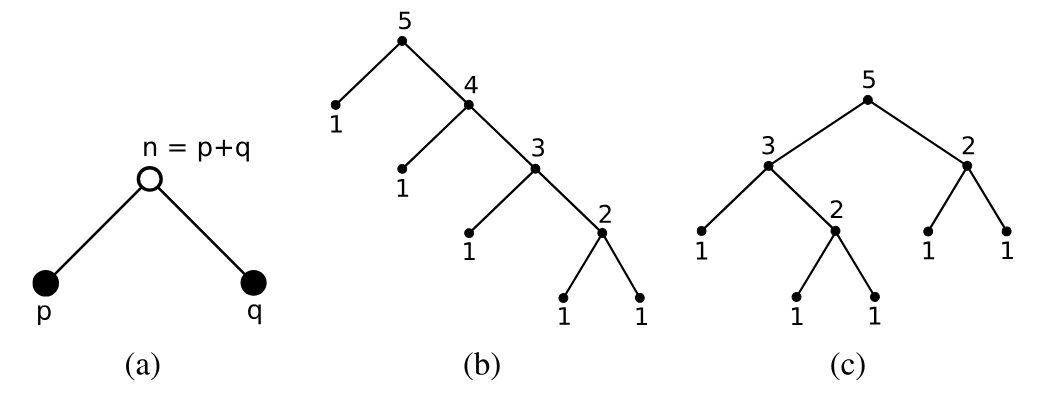
\includegraphics[width=0.7\textwidth]{images/trees.png}
    \captionsetup{justification=centering}
    \caption{Possible decompositions in tree form \cite{qureshi_generation_2011}}
            All of the possible decompositions of the FFT represented as powers of two as part of a tree.
    \label{fig:trees}
\end{figure}

The work especially explores the use of specific decomposition which would reduce the calculation effort. The various decompositions of the \ac{dft} a shown in a tree with the different smaller \ac{fft}s as powers of two (see figure \ref{fig:trees}). Implemented in hardware some of the phase rotations between the different stage become trivial for calculations as they turn out to be one or zero.  As the table in figure \ref{fig:rotator_table} shows various algorithm with different amounts of trivial rotators are possible. The rotators are shown as roots of unity were a larger number indicates a more complex calculation.  It is shown that larger rotators should be placed later in the algorithm has they demand a change in the data word length in the \ac{fpga} \cite{qureshi_generation_2011}.\par

\definecolor{Silver}{rgb}{0.752,0.752,0.752}
\definecolor{Gray}{rgb}{0.501,0.501,0.501}

\begin{table}
\centering
\resizebox{0.4\textwidth}{!}{
\begin{tblr}{
  cells = {c},
  cell{1}{2} = {c=3}{},
  cell{3}{2} = {Silver},
  cell{3}{3} = {Silver},
  cell{3}{4} = {Silver},
  cell{5}{3} = {Silver},
  cell{5}{4} = {Silver},
  cell{7}{3} = {Silver},
  cell{7}{4} = {Silver},
  cell{9}{3} = {Silver},
  cell{9}{4} = {Silver},
  cell{11}{2} = {Silver},
  cell{11}{3} = {Silver},
  cell{11}{4} = {Silver},
  cell{12}{2} = {Gray},
  cell{13}{2} = {Silver},
  cell{13}{3} = {Silver},
  cell{13}{4} = {Silver},
  cell{14}{3} = {Gray},
  cell{15}{3} = {Silver},
  cell{15}{4} = {Silver},
  cell{17}{3} = {Silver},
  cell{17}{4} = {Silver},
  cell{18}{2} = {Silver},
  cell{18}{4} = {Gray},
  cell{19}{3} = {Silver},
  cell{19}{4} = {Silver},
  cell{21}{2} = {Silver},
  cell{21}{3} = {Silver},
  cell{21}{4} = {Silver},
  vlines,
  hline{1-3,22-23} = {-}{},
  hline{4-21} = {2-4}{},
}
                    & Algorithm &         &         \\
Stage               & 10-20-10  & 12-20-8 & 16-20-4 \\
1                   & W4        & W4      & W4      \\
2                   & W8        & W16     & W16     \\
3                   & W32       & W4      & W4      \\
4                   & W4        & W256    & W256    \\
5                   & W1024     & W4      & W4      \\
6                   & W4        & W16     & W16     \\
7                   & W8        & W4      & W4      \\
8                   & W32       & W4096   & W65k    \\
9                   & W4        & W4      & W4      \\
10                  & W1M       & W16     & W16     \\
11                  & W4        & W4      & W4      \\
12                  & W8        & W1M     & W256    \\
13                  & W32       & W4      & W4      \\
14                  & W4        & W16     & W16     \\
15                  & W1024     & W4      & W4      \\
16                  & W4        & W256    & W1M     \\
17                  & W8        & W4      & W4      \\
18                  & W32       & W16     & W16     \\
19                  & W4        & W4      & W4      \\
{Trivial\\rotators} & 8         & 10      & 10      
\end{tblr}
} % Ende \resizebox
\caption{Algorithm variants with different decompositions \cite{kanders_1_2019}}
        Overview over the rotators of different decompositions as roots of unity. Trivial rotators are marked with light grey. The largest rotator is marked with dark grey.
\label{fig:rotator_table}
\end{table}

With this considerations in mind the 12-20-8 algorithm with two to the power of 4 or 5 as the smallest calculation unit is chosen. The algorithm is implemented into an \ac{fpga} using special units for the rotators. The design only uses up to 12 percent of calculation and I/O units but 67 percent of the memory units of the \ac{fpga}. This makes this approach as a solution for the large \ac{fft} for multiple channels insufficient as the run time is with 0.5ms above the maximum run time of 0.11 ms. Due to the high memory requirements it is not possible to run the whole algorithm in parallel to make up for the long run time \cite{kanders_1_2019}.

\section{Block-by-Block Configurable Fast Fourier Transform}
In a white paper Xilinx engineers describe a way to implement a 4096 datapoint \ac{fft} with little space consumption on the AI Engines. This approach stands out due to its ability to adjust the size and configuration of the \ac{fft} depending on the specific requirements of a given task. The \ac{fft} is therefore split into multiple building blocks, hence the name block-by-block configurable \ac{fft}. This blocks represent smaller \ac{fft}s due to a split up according to the Cooley-Tukey algorithm. In figure \ref{fig:packet_array} this decomposition is shown. The grey boxes represent one AI Engine tile there. All of the \ac{fft} blocks can be configured for a certain transform size by an control word. To get data to these blocks the implementation uses a combination of an AXI stream and the AI Engines packet switching. For the calculation int32 values are used to save up memory for precalculated twiddle factors \cite{block_by_block}.\par

\begin{figure}[h]
    \centering
    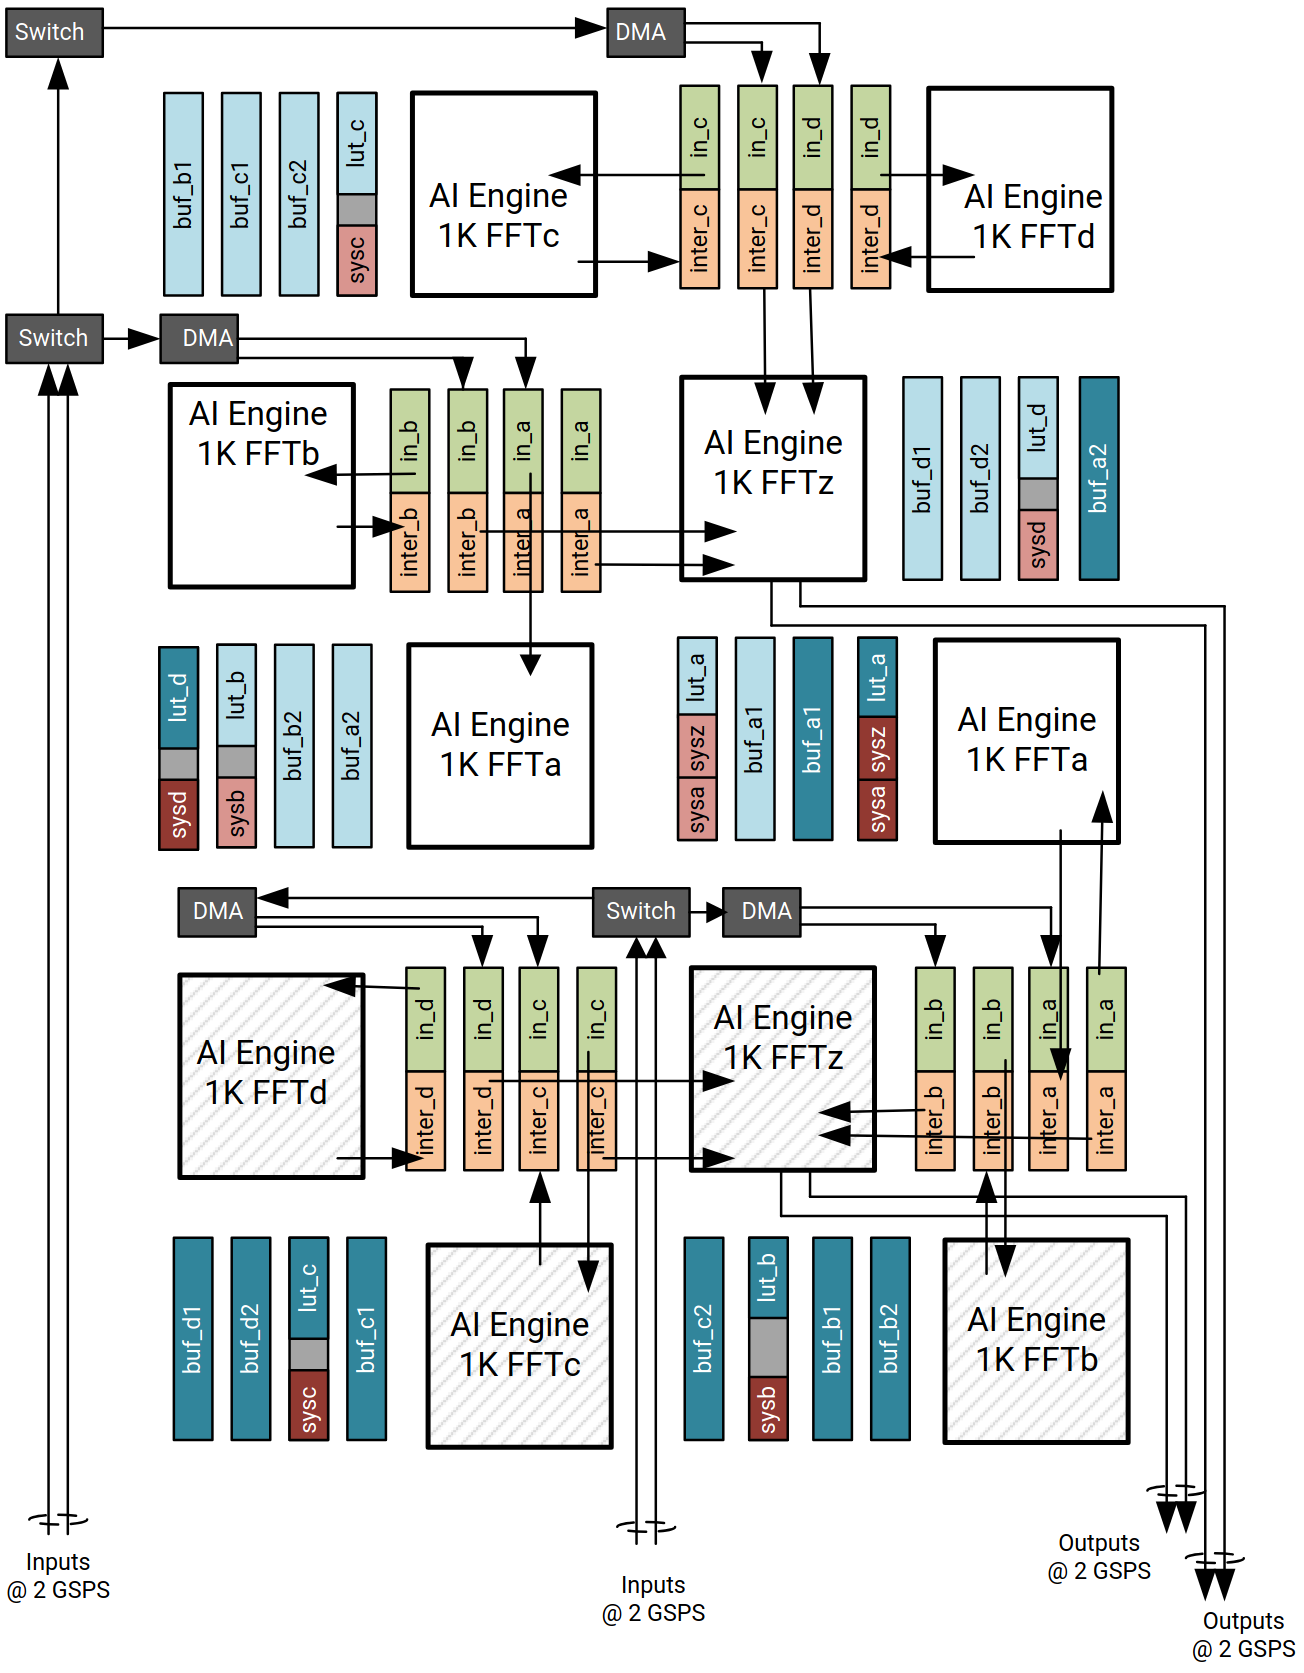
\includegraphics[width=0.65\textwidth]{images/packet_array.png}
    \captionsetup{justification=centering}
    \caption{Two of the described modules are packet together to achieve higher throughput \cite{block_by_block}}
            Schematic of two 5 AI Engine modules packed together. The utilization of the memory banks with the different buffers and the dataflow from and to them is shown.
    \label{fig:packet_array}
\end{figure}

In terms of performance metrics, the Block-by-Block Configurable Fast Fourier Transform has a throughput of 1.85 GSPS for a 4096 point \ac{fft} running on 5 AI Engines. This AI engines can be packed densely as shown in figure \ref{fig:packet_array}. to achieve higher throughput. This approach is very useful for antenna arrays in mobile communications or radar where a lot of smaller \ac{fft}s needs to be performed for analysis reasons. For this work this isn't sufficient. The goal is to achieve a throughput of 2.61 GSPS over an $2^{18}$ point \ac{fft}. Although the throughput could be easily achieved by combining multiple of the arrays, the size of the \ac{fft} isn't that easy to increase. All of the buffer need to be changed so the larger \ac{fft} can fit into them as the current buffer structure cant be scaled up. The general structure of this approach is very promising for this thesis and will be considered as a foundation for a new algorithm \cite{block_by_block}.


\section{Vitis AI Engine Libraries }
Xilinx offers a library especially for \ac{fft} implementations which combine \ac{pl} and AI Engines. It is implemented similar to the Block-by-Block Configurable Fast Fourier Transform by using a the Cooley-Tukey approach placing multiple smaller \ac{fft}s in parallel on the AI Engines. All of the twiddle factors and phase rotations are calculated in advance as this is a common method for optimization in \ac{fft}s. The size of the \ac{fft} is not configurable during run time. It is configured with a templated function during the programming stage. An arbitrary size for the \ac{fft} can be chosen. Furthermore certain parallization flags can be set which allow the mapping to a specific amount of tiles to increase the throughput \cite{vitis_libs}.\par
The design of the \ac{fft} has large memory requirements for buffering and twiddle and phase rotation storage. This imposes constraints on the size that can be implemented with this library. The performance analysis conducted by Xilinx uses a maximum \ac{fft} size of 65536 with the cint16 datatype for their test. For an \ac{fft} with an higher precision with the cfloat datatype only a size of 1024 is tested \cite{fft_libs}. This size alone renders this library insufficient for the use in this thesis as the higher precision of the cfloat datatype is needed by the constraints of the imaging algorithm. Even with out the memory constraints this \ac{fft} only reaches a throughput of 407 MSPS which is also below the needed throughput. For the use of this library in multi static imaging, the memory usage needs to be optimized to enable larger \ac{fft}s with higher precision \cite{fft_libs}. 
\chapter{Design}\label{ch:design}
%Is the central chapter of the work. Here the goal as well as the own ideas, evaluations, design decisions are presented. It can be worthwhile to play through different possibilities and then explicitly justify why one has chosen a particular one. This chapter should - at least in keywords - already be sketched out and written in keywords when a design is first defined. However, in a normal course of work, something will constantly change. The chapter must not become too detailed, otherwise the reader will be bored. It is very important to find the right level of abstraction. When writing, one should pay attention to the reusability of the text. (8-20 pages)

% 1. Decision: why AIE instead of DSP (mention config_block_design here) x
% 2. Decision: why Cooley-Tukey instead of reversed index technique (latter one used on one single kernel) x
% 3. Decision: what specific Cooley-Tukey decomposition x?
% 4. D: Using pkt streaming for data partition
% 5. D: Using PL for reordering between stages
% 6. D: Pipeling of the stages (maybe later)
% 7. D: Stream pkts into buffers (stalling problem) / why no ping pong buffers
% 8. D: precalculated twiddle factors
% 9. D: how si the vector unit used

This chapter provides a detailed explanation of the design of the \ac{fft} implementation, with a focus on both hardware and software decisions. Beforehand an the system requirements described in section \ref{sec:req}, which are driven by the need to support large Fourier Transforms for synthetic aperture as described in section \ref{sec:fbi}, will be translated into constraints for the design. The overall goal will be to calculate 256 different \ac{fft}s with a size of $2^{18}$ each within 30 ms.

\section{Constraints}
As outlined in the initial design goals, the algorithm developed in this thesis aims to enable real-time processing capabilities for a system with 256 receivers and 10 senders, requiring a high level of performance for \ac{fft} computation. For each frame of the desired 30 frames per second stream, each of the 256 receivers must process an \ac{fft} based on  $2^{18}$ data points sampled from a 4 ms signal at 65.536 MHz with a 16-bit resolution per data point. This translates to a total of 256 \ac{fft}s needing completion within the 30 ms window.\par
In light of these goals, several constraints emerge, notably in terms of memory and processing speed. Each $2^{18}$-point \ac{fft} utilizes 64-bit (8 bytes) precision per complex data point, given the \ac{adc}'s fixed bit resolution and property of the complex number to have a real and an imaginary part. This leads to a memory demand of approximately 2.1 MB per \ac{fft}. As discussed in Section \ref{sec:versal}, the Versal platform's AI Engines provide a combined memory capacity of 12.8 MB, theoretically allowing for four concurrent \ac{fft} computations. However, to manage memory allocation effectively across AI engine tiles and account for data streaming and precomputed values, the design optimizes resource allocation by processing one \ac{fft} at a time. To compensate for this all the \ac{fft}s need to be calculated sequentially within the 30 ms limit. The further analysis of this issue will show that this becomes possible as now more calculation units are now available for this particular calculation step.\par
With this design decision, timing constraints intensify. To maintain the 30 ms target, each \ac{fft} must complete within 0.117 ms. Operating at 1.25 GHz, the AI Engines provide a processing window of 146,250,000 instructions per \ac{fft}. These constraints shape the algorithm optimization, guiding the memory and processing flow throughout the system. The following sections detail the architectural choices implemented to meet these stringent requirements, focusing on efficient memory management and the distribution of computational resources across the AI Engine array.

\begin{figure}[h]
    \centering
    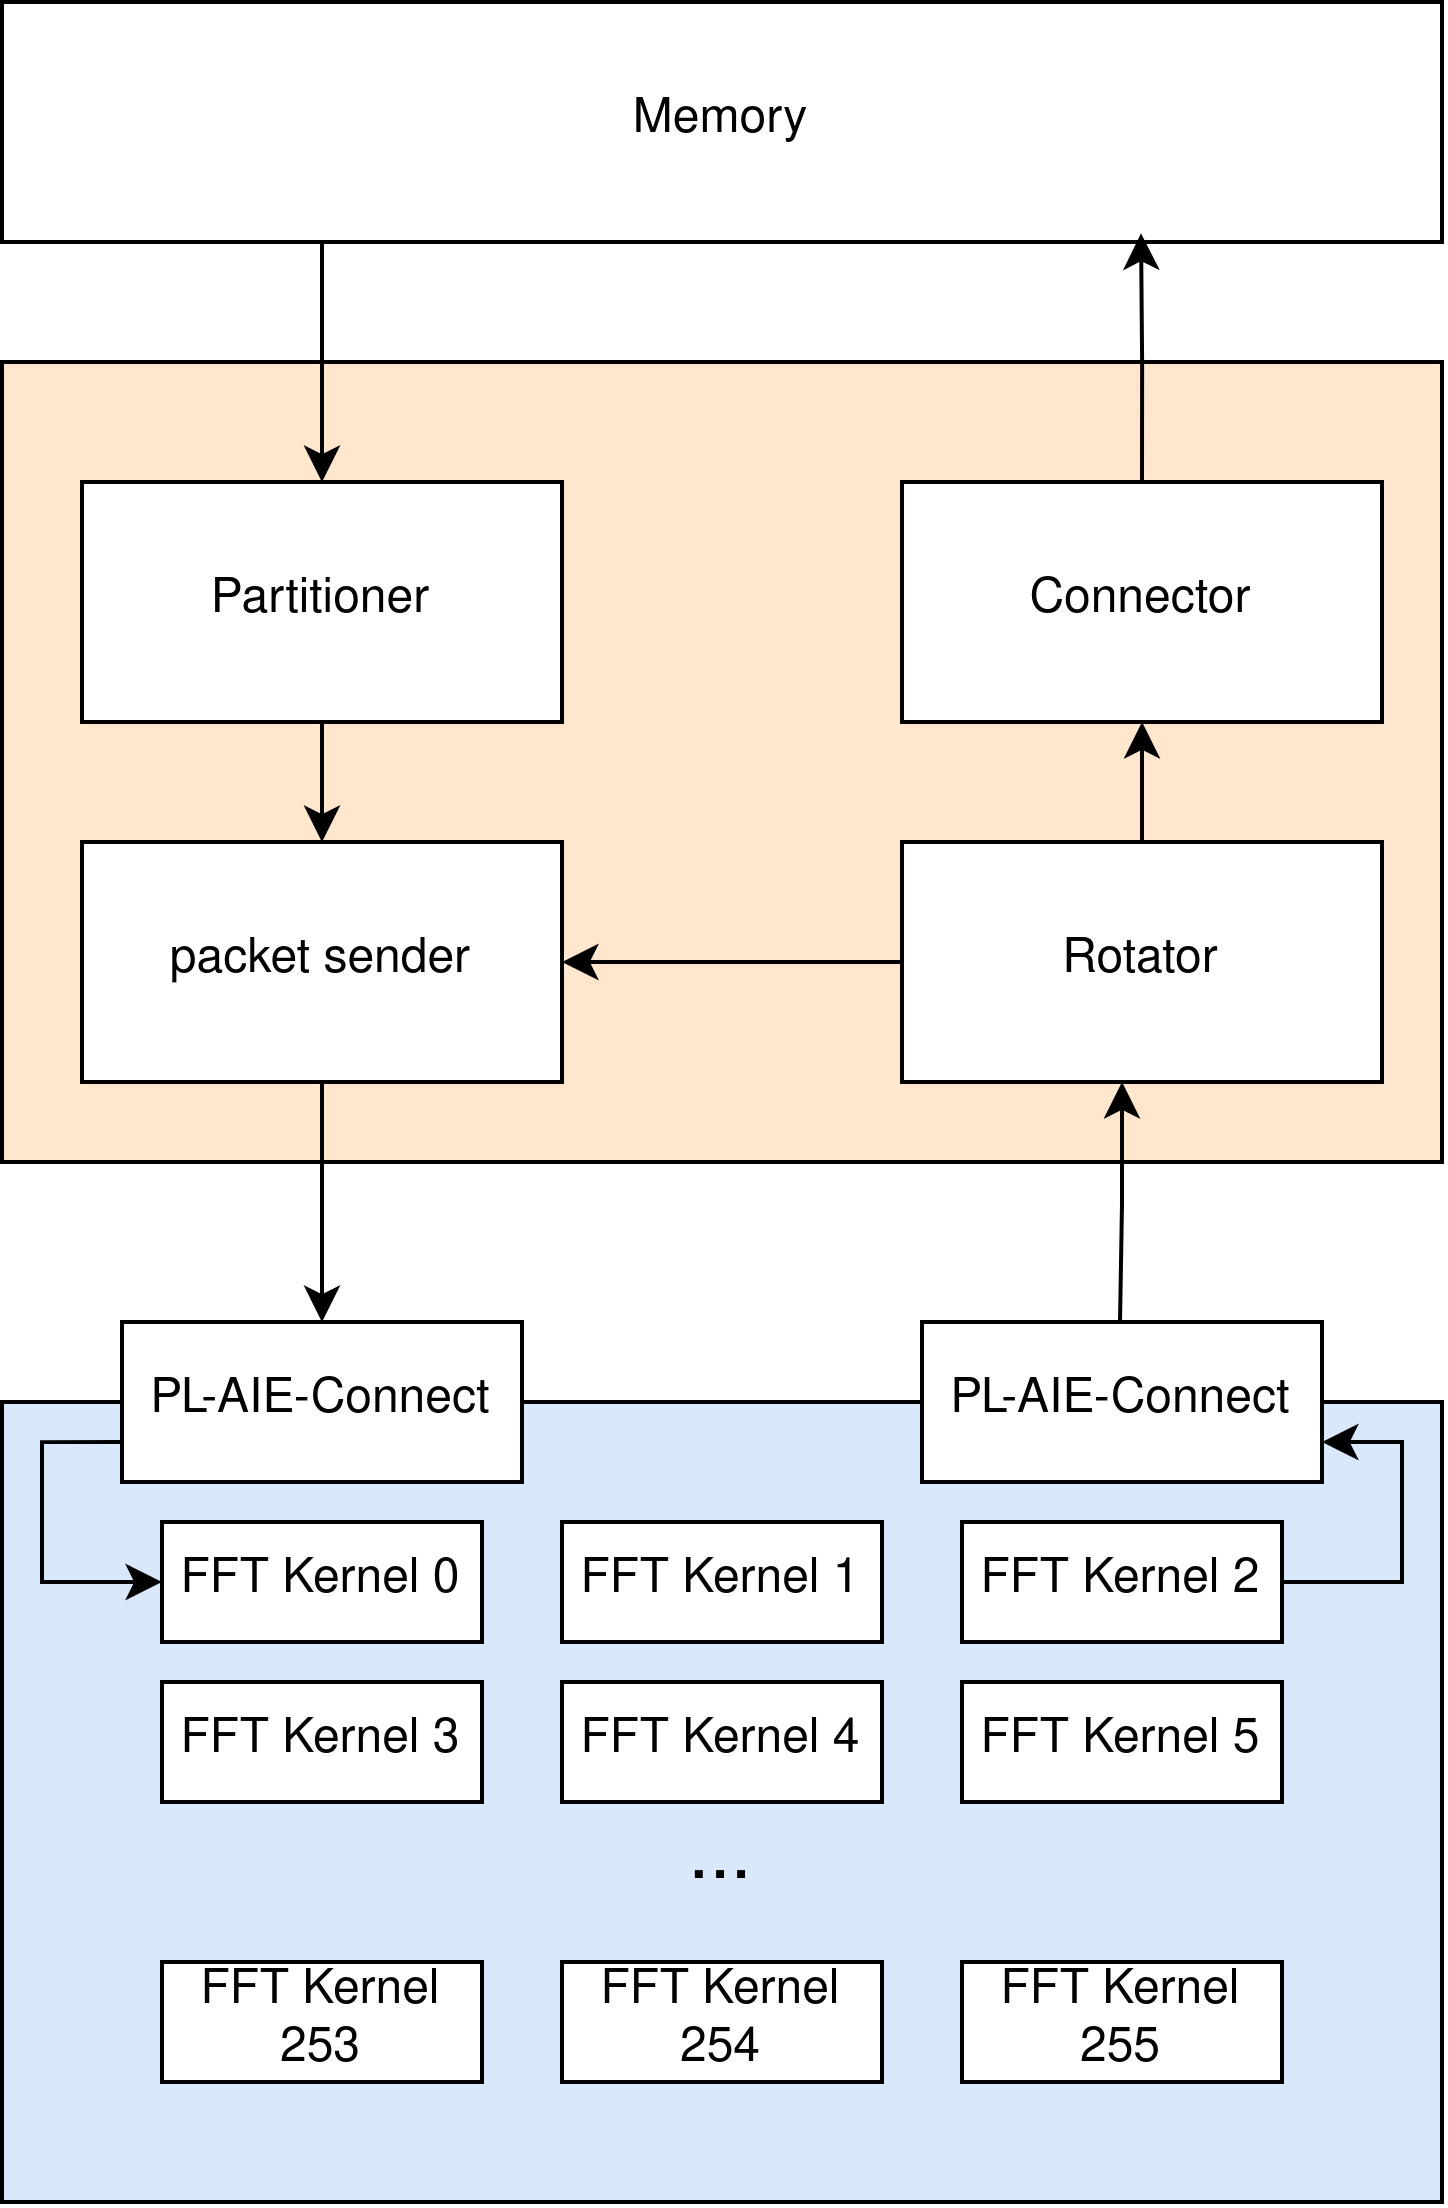
\includegraphics[width=0.5\textwidth]{images/overview.png}
    \captionsetup{justification=centering}
    \caption{Overview over the major building blocks in \ac{pl} and AI Engines}
        The general structure of the algorithm divided into its main building blocks. The yellow box shows the parts located in the \ac{pl} while the blue box outlines the kernels within the AI Engines.
    \label{fig:overview}
\end{figure}

\section{Overall Structure}
A straightforward approach to reduce the number of sequential instructions is to parallelize the algorithm. While this does not necessarily decrease the total number of instructions, it does reduce the number of instructions that need to be executed sequentially within the specified time frame. This is because two instructions computed in parallel contribute only once to the time constraint. An effective way to parallelize an \ac{fft} is by utilizing the Cooley-Tukey algorithm described in section \ref{sec:ft}. For practical reasons, I chose to decompose the $2^{18}$-point \ac{fft} into smaller 1,024-point and 256-point \ac{fft}s. This structure allows to fully utilize the memory of one AI Engine tile which features four 8kb memory ranks. The buffer for the 1024-point \ac{fft} would be exactly 8kb large. This allows to fit the input and output buffer of one kernel exactly on to one memory bank each. Further this allows to reuse a the same memory structure for the 256-point \ac{fft}s as they are a divisor of 1024.In the following sections, I will describe the overall algorithm design, detailing how this decomposition is employed to optimize performance while meeting the design constraints.\par
The architecture of the system is divided into two key components: the \ac{pl} and the AI engines. Each of these components is further subdivided into smaller functional units. The central idea behind this design is the dataflow between these two components. Initially, data is streamed from the DDR memory through the \ac{pl} to the AI engines, where the first stage of the \ac{fft} computation is performed. Once this initial computation is completed, the data is transferred back to the \ac{pl}, where it is reordered in preparation for the second stage of processing. Subsequently, the data is streamed again into the AI engines, where the second stage of the \ac{fft} computation takes place. Finally, the processed data is written back to memory through the \ac{pl}. This dataflow structure is designed to optimize the utilization of both the \ac{pl} and the AI engines, ensuring efficient processing while adhering to the timing constraints discussed in previous sections.\par
As previously discussed, the \ac{pl} is responsible for managing the interaction with the RAM and controlling the data stream for the AI engines. The \ac{pl} consists of four main components, as illustrated in figure \ref{fig:overview}.The first component, the Partitioner, is primarily responsible for interacting directly with the DDR memory, handling the loading and reordering of input data. This ensures that the data is properly prepared for the subsequent stages of computation.The Packet Sender is the second component and can receive data streams from two sources: either from the Partitioner or from the Rotator. It packages these data streams into packets, which are then streamed to the AI engines for \ac{fft} computation.The Rotator, another key component, takes the data stream returned from the AI engines after the first \ac{fft} stage. It can either pass the data directly to the Connector or reorder it before sending it back to the Packet Sender for further \ac{fft} processing.\par
Finally, the Connector is responsible for writing the final \ac{fft} results back to the DDR memory. It abstracts the logical processing from memory access, ensuring a clear separation between the computational processes and the data storage operations.Together, these components coordinate the flow of data between memory, the \ac{pl}, and the AI engines, facilitating efficient handling of the large data volumes required for the \ac{fft} computations.\par
The second major building block, the AI engines, are organized differently than the \ac{pl}. They are connected to the \ac{pl} via specialized connection tiles (see section \ref{sec:versal}). As illustrated in the schematic, these connection tiles specifically link to the Packet Sender and Rotator. Each of these two building blocks is connected with 8 streams to these tiles. The connection tiles take the eight data streams they receive and split them into 32 packets each, which are then streamed to individual AI engine tiles. This configuration utilizes a total of 256 AI engine tiles. Each of these tiles implements the same kernel, which is capable of executing either a 1024-point \ac{fft} followed by a phase rotation or four separate 256-point \ac{fft}s. The appropriate mode is selected using a control word embedded in the data stream. After the computations are completed, the data is streamed back to the connection tiles, where the individual streams are repackaged into eight data streams before being sent back to the \ac{pl}. This structured approach to the AI engines enhances parallel processing capabilities, allowing for efficient execution of \ac{fft} calculations while maintaining a streamlined connection to the \ac{pl}.

\begin{figure}[h]
    \centering
    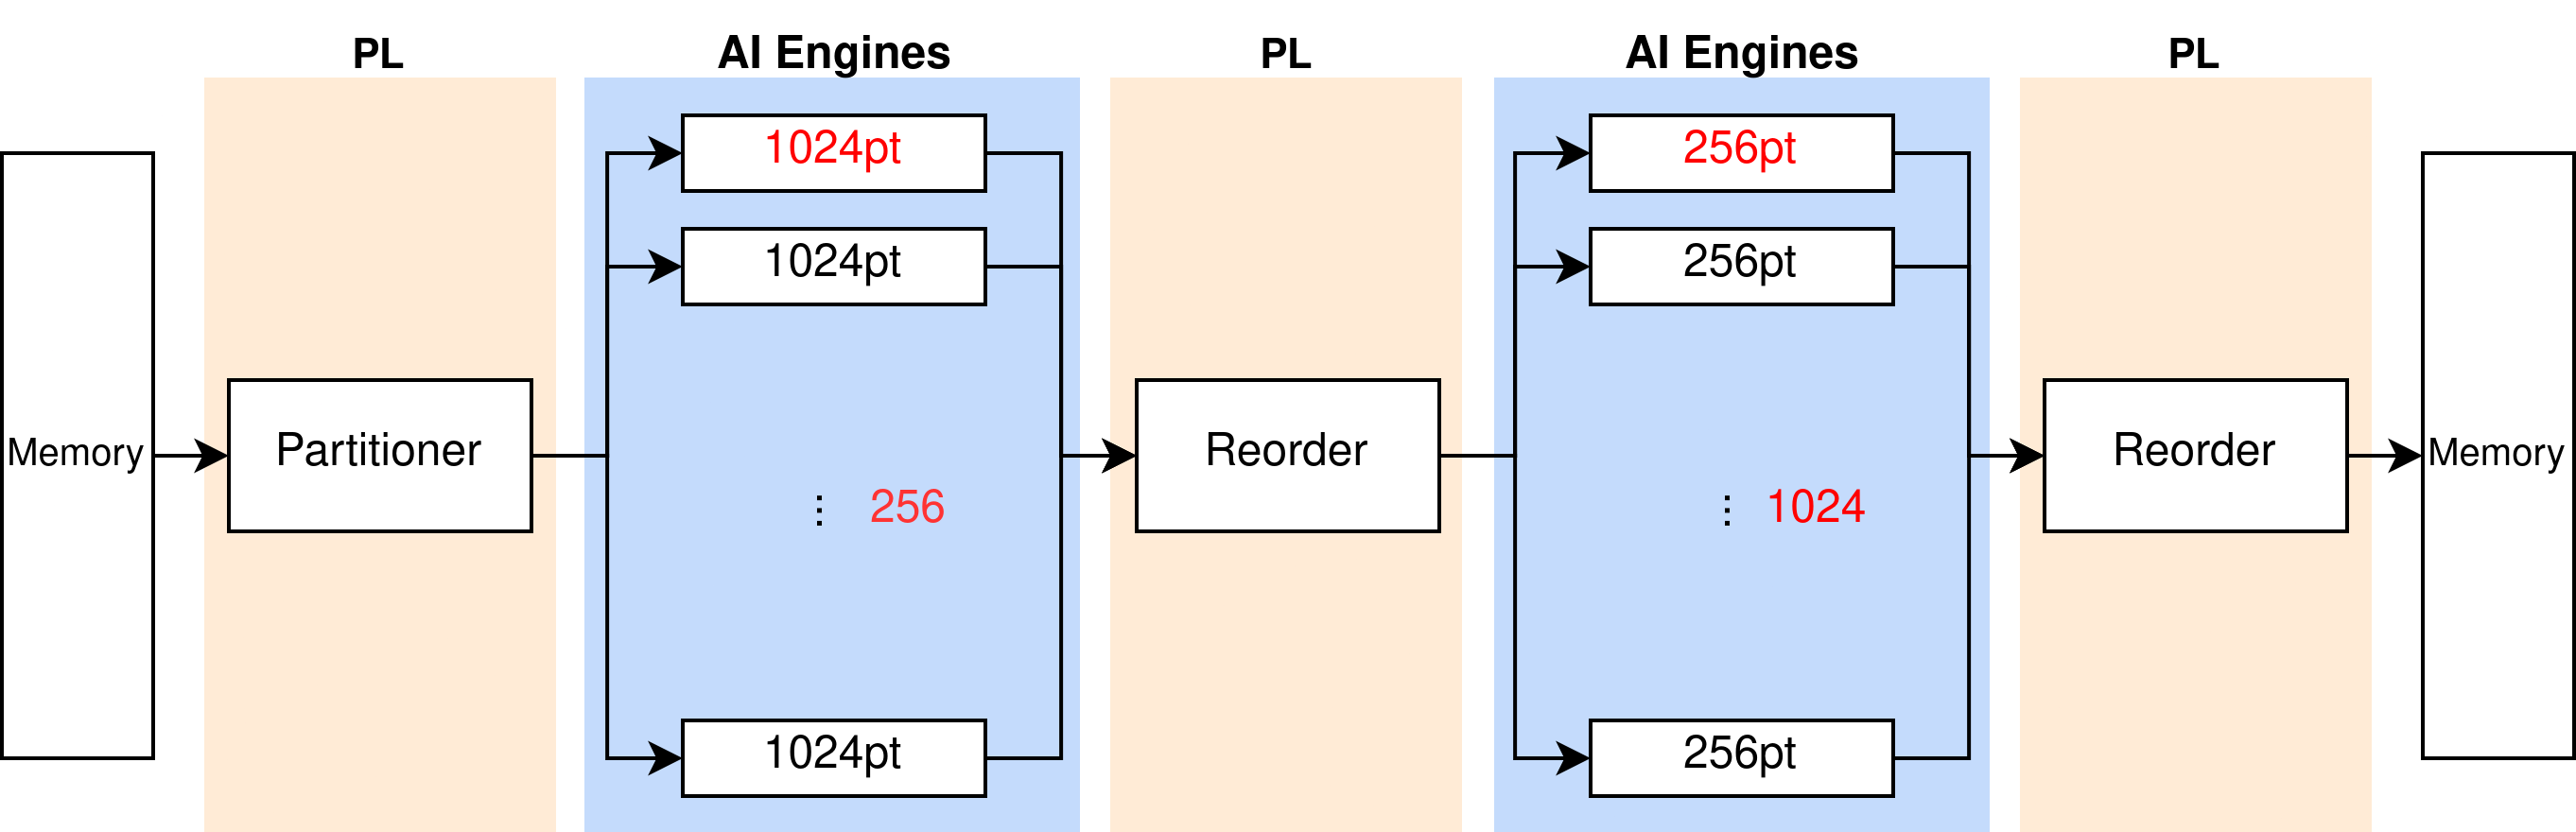
\includegraphics[width=1.0\textwidth]{images/prototype.png}
    \captionsetup{justification=centering}
    \caption{Pipelined algorithm design}
            Every vertical slice is independent from the other parts of the system. Yellow slices are implemented on the PL while blue slice are implemented as kernels on the AI Engines.
    \label{fig:pipelined}
\end{figure}

\section{Sequential or pipelined design}
As illustrated by the color coding in figure \ref{fig:overview}, the \ac{pl} (yellow )and the AI engines (blue) represent two distinct components that utilize different hardware. This distinction raises an important question regarding the potential for pipelining between these two stages. Implementing a pipelined approach could alleviate some of the design constraints discussed earlier, as the runtime constraint would no longer apply to the entire design, but only to the slowest pipeline stage. Figure \ref{fig:pipelined} presents a design that incorporates a pipelined approach. However, this design is not without its drawbacks and challenges, which will be explored in detail in this section.\par
The design depicted in the schematic closely resembles the previously described architecture. It features building blocks within the \ac{pl} that are responsible for partitioning and reordering data, alongside building blocks within the AI engines that perform the actual computations. The primary distinction in this design is that each building block operates as its own instance. This means that every implementation of a building block in the \ac{pl} occupies dedicated hardware resources, enabling it to run in parallel with other instances of the same block. In the schematic, this parallelism is represented by the slices, each symbolizing an independent implementation, in contrast to the shared implementations shown in figure \ref{fig:overview}. This concept similarly applies to the AI engines, where each kernel is implemented on its own tile. This architectural design facilitates a pipelined approach, allowing each of the vertical stages in figure \ref{fig:pipelined} to operate concurrently with the other stages. Such parallel execution enhances the overall throughput of the system and improves efficiency in handling the computational load.\par
One significant limitation of this design is resource allocation, especially considering the increased resource demands of the AI engines. While the \ac{pl} provides ample resources to implement multiple instances of identical building blocks, the AI engines face constraints due to the limited number of available tiles and the restricted memory capacity per tile. As outlined in section \ref{sec:versal}, each tile has a maximum memory of 32 KB. Not all of this memory can be allocated for storing data on which the \ac{fft} will be executed. As described in more detail in section \ref{sec:imp}, each AI engine requires two buffers—one for incoming unprocessed data and one for processed data. Consequently, each buffer is limited to only 8 KB of memory, with the remaining memory allocated for other internal data structures required by the algorithm. This constraint allows only the decomposition of the \ac{fft} into a maximum of 1024 and 256 \ac{fft}s. The assignment of AI engines follows accordingly: in the first stage, 256 tiles are allocated for the 1024 \ac{fft}s, while the second stage would ideally require 1024 tiles for the 256 \ac{fft}s. With only 400 tiles available, this configuration is infeasible. Even if four 256 \ac{fft}s were placed on each tile to fully utilize the 8 KB of memory in each second-stage kernel, 256 AI engines would still be needed for the second stage. This would result in a total of 512 AI engines, exceeding the 400-tile limit. Due to these limitations, it is not possible to pipeline the design for such a large \ac{fft} \cite{AMD_a_aie}.

\section{Programmable Logic kernels}
A critical question arising from the proposed design is the rationale behind incorporating \ac{pl} at all. At first glance, it may seem more practical to confine the design within the AI engines to avoid complications associated with differing clock domains and the need for multiple streaming interfaces between various hardware components. However, the use of \ac{pl} remains essential due to the specific structure of the data that needs to be processed. As described in section \ref{sec:ft}, the data must be reordered between the two stages of the \ac{fft} in such a way that the index value of the output from the first stage directly corresponds to the \ac{fft} that will process this output in the second stage. Specifically, the first output of the first \ac{fft} from the first stage serves as the first input for the first \ac{fft} of the second stage. Similarly, the second output of the first \ac{fft} from the first stage becomes the first input for the second \ac{fft} of the second stage, while the first output of the second \ac{fft} from the first stage is routed as the second input for the first \ac{fft} of the second stage. Thus, the \ac{fft} number from the first stage designates the index number of the corresponding \ac{fft} in the second stage, while the index number within the first stage identifies the specific \ac{fft} block where the second stage will be processed. This concept is illustrated in figure \ref{fig:stage_reorder}, highlighting the importance of the \ac{pl} in efficiently managing the data reordering necessary for the \ac{fft} computations.\par
As illustrated in this scheme, the proposed memory access pattern is highly suboptimal, particularly considering that the various \ac{fft} blocks are distributed across different tiles. This inefficiency underscores the necessity of utilizing \ac{pl} in the design. By streaming data into the \ac{pl}, it becomes feasible to achieve data locality by storing the different results in Block RAM (BRAM) blocks that are directly interconnected. This approach allows for some degree of locality, even in the presence of highly irregular data structures. Additionally, it is worth noting that reordering algorithms are well-established in the context of \ac{fpga}s and \ac{pl}. These algorithms can be effectively leveraged to enhance the performance of the \ac{fft} computations, potentially leading to further speed improvements in the algorithm. Having discussed the rationale for incorporating \ac{pl}, I will now explore the single \ac{pl} kernels, the Partitioner, the Packetsender, the Rotator and the Connector in more detail.\par

\begin{figure}[h]
    \centering
    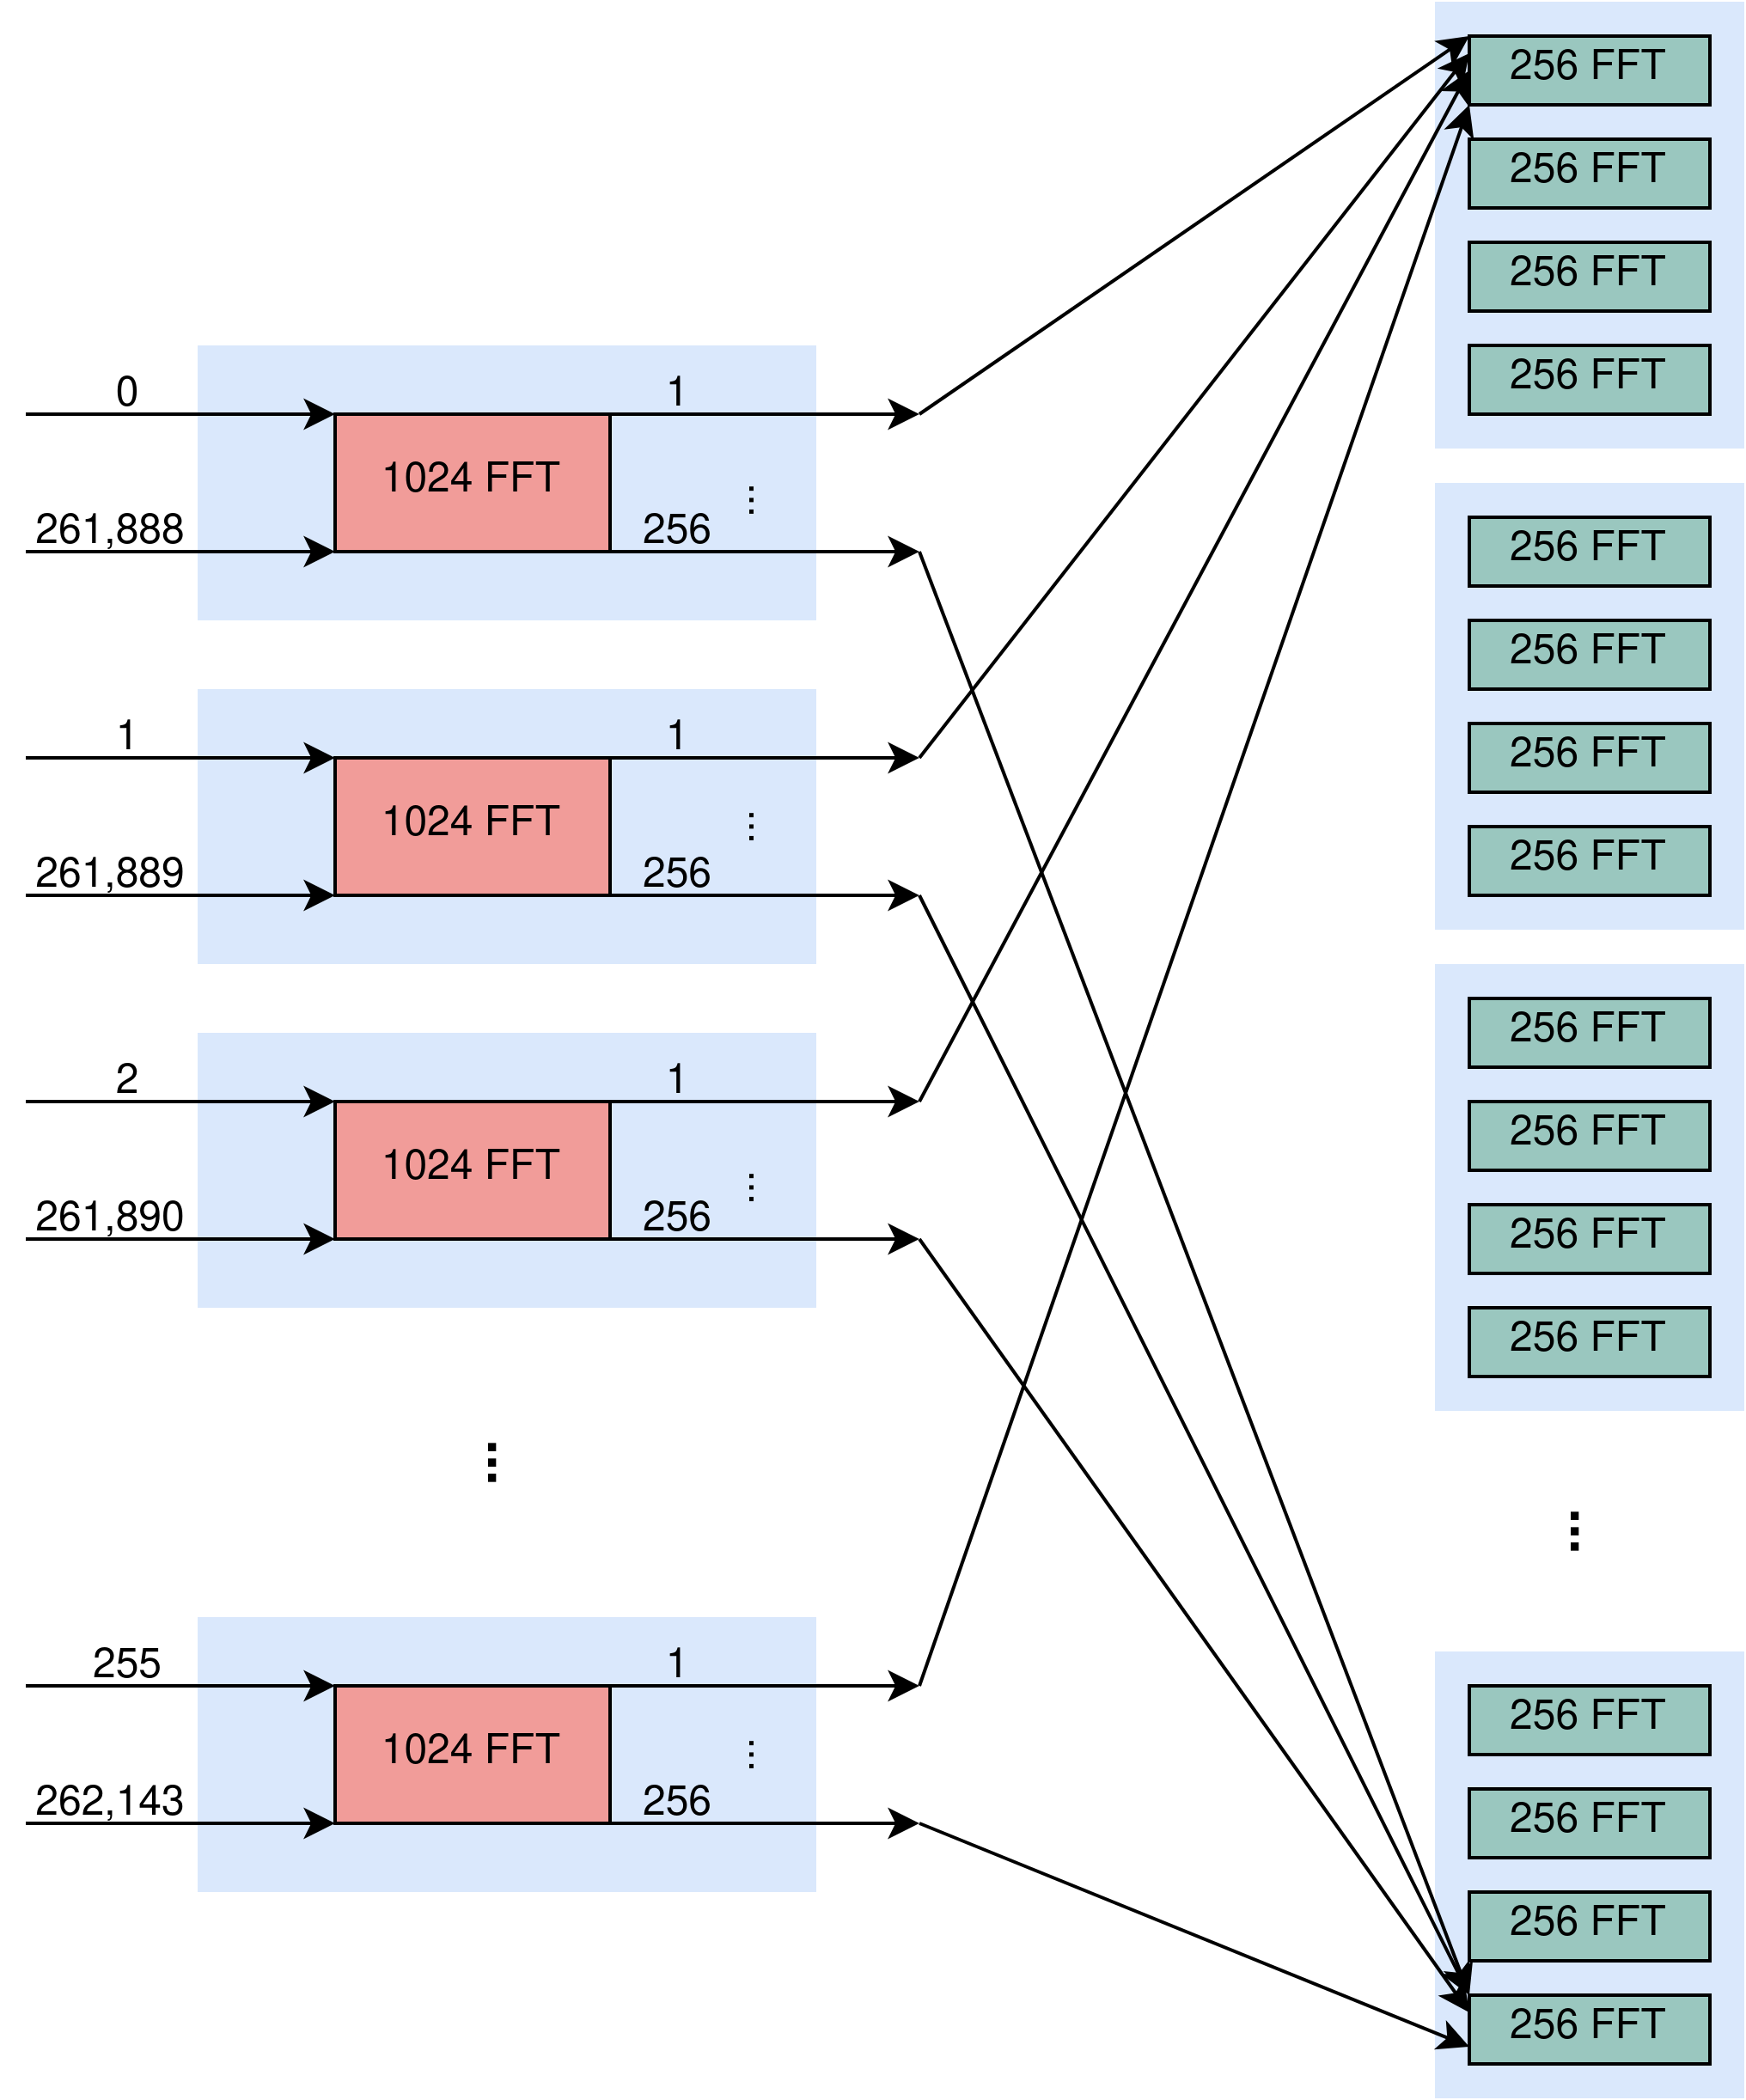
\includegraphics[width=0.7\textwidth]{images/stage_reorder.png}
    \captionsetup{justification=centering}
    \caption{Reorder scheme between stages}
            Every light blue box represents one AI Engine tile. It shows how the memory of one tile of the second stage is composed of multiple single memory entries from the first stage.
    \label{fig:stage_reorder}
\end{figure}

\subsection{Partitioner}
The Partitioner serves as a wrapper for interacting with the DDR memory, effectively encapsulating memory access from the rest of the design. This encapsulation enables the algorithm to be adapted for real-world scenarios without necessitating modifications to integral components. The primary functions of the Partitioner include loading data from DDR memory and reordering it for optimal use in the AI engines. The reordering schema utilized by the Partitioner is illustrated in figure \ref{fig:input_reorder}. Initially, the data is segmented into frames of 1024-point values for the first stages of the \ac{fft}. Each value is extracted in 256-step increments from the original memory to satisfy the input order constraints of the \ac{fft} algorithm. Once reordered, the data frame is divided into eight streams, with each stream containing 32 \ac{fft} packets. Specifically, the first stream carries packets 0 to 31, the second stream carries packets 32 to 63, and this pattern continues for the remaining streams up to packet 255. Importantly, during this splitting process, no additional information about the \ac{fft} is incorporated. This task is managed by the subsequent building block, the Packet Sender, to which the eight output streams are connected.

\begin{figure}[h]
    \centering
    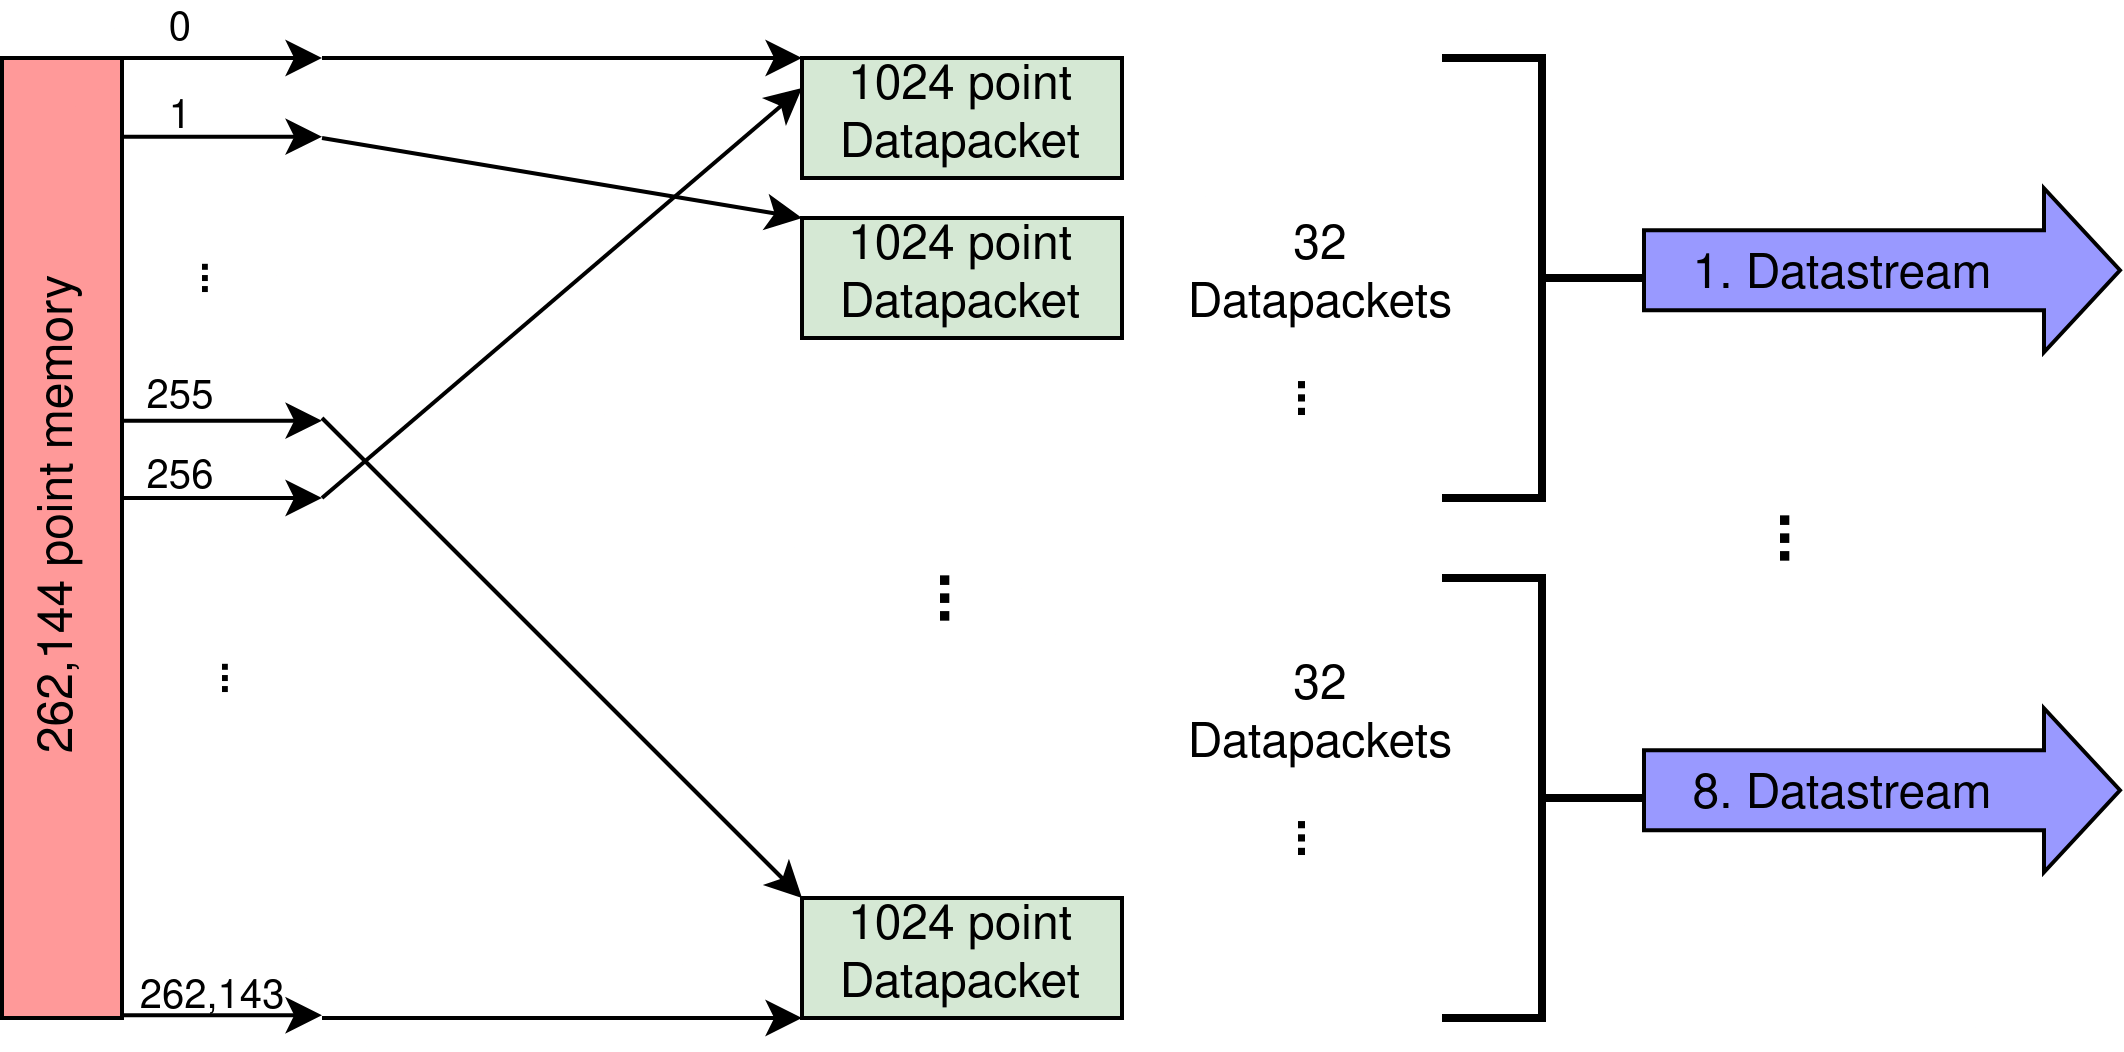
\includegraphics[width=0.7\textwidth]{images/input_reorder.png}
    \captionsetup{justification=centering}
    \caption{Reordering in the Partitioner}
            It is shown how the datastreams that are send from the Partitioner are created within. 32 datapackets are composed into one datastream.
    \label{fig:input_reorder}
\end{figure}

\subsection{Packetsender}
As its name implies, the Packetsender is responsible for constructing real data packets and transmitting them to the AI engines. This mechanism consists of two primary components: first, the streaming of data to the AI engine connection tiles via the AXI interface, and second, the streaming of data from those connection tiles to the tiles housing the AI engine cores. Since the second component is closely tied to the data packaging occurring outside the AI engines, it will also be discussed in this section.\par
In the first part of the process, a streaming connection is established between the connection tiles and the Packet Sender. The primary data for these streams can originate from either the Partitioner or the Rotator, allowing the Packet Sender to multiplex between the two sources. As explained in section \ref{sec:versal}, a single stream can be split into a maximum of 32 individual streams. To accommodate the data requirements for all 256 kernels, eight streams are used, each carrying data for 32 individual streams. Each of these individual streams contains 1,024 data points for a single \ac{fft}. To meet these requirements, the Packet Sender reads 1,024 values from a stream—either from the Partitioner or Rotator input—and appends a header that specifies the destination tile. The destination information is generated during the compile time of the AI engine kernels and is subsequently passed to the other building blocks as a table. Additionally, a control word is included with the transmitted data, providing information on which \ac{fft} stage the algorithm is currently executing, thereby enabling the correct branching within the AI engines. To conclude each packet, a stop byte is appended at the end of the data frame.

\subsection{Rotator}
The Rotator operates as an intermediary layer between the first and second stages of the \ac{fft}. Its primary function is to reorder the outputs from the first stage or prepare the data for memory write-back. The Rotator processes data received from eight streams, each connected to the connection tiles of the AI Engines. If the data originates from the first stage of the \ac{fft}, it is reordered and buffered in BRAM according to the memory scheme shown in Fig. X. Conversely, if the data is from the second stage, a reverse index reordering scheme is applied to ensure the correct output order. In the first scenario, the data is transmitted through eight streams to the Packet Sender, which then streams the data back into the AI Engines. The data splitting scheme follows a pattern similar to that used by the Partitioner, with the key difference being that a single 1024-point dataframe now holds four 256-point dataframes. When data originates from the second stage of the \ac{fft}, it is sent via a single stream to the Connector. The Connector executes a straightforward memory write-back operation for all received elements. This process encapsulates memory access, isolating it from the rest of the logical design, similar to the approach employed by the Partitioner.

\begin{figure}[h!]
    \centering
    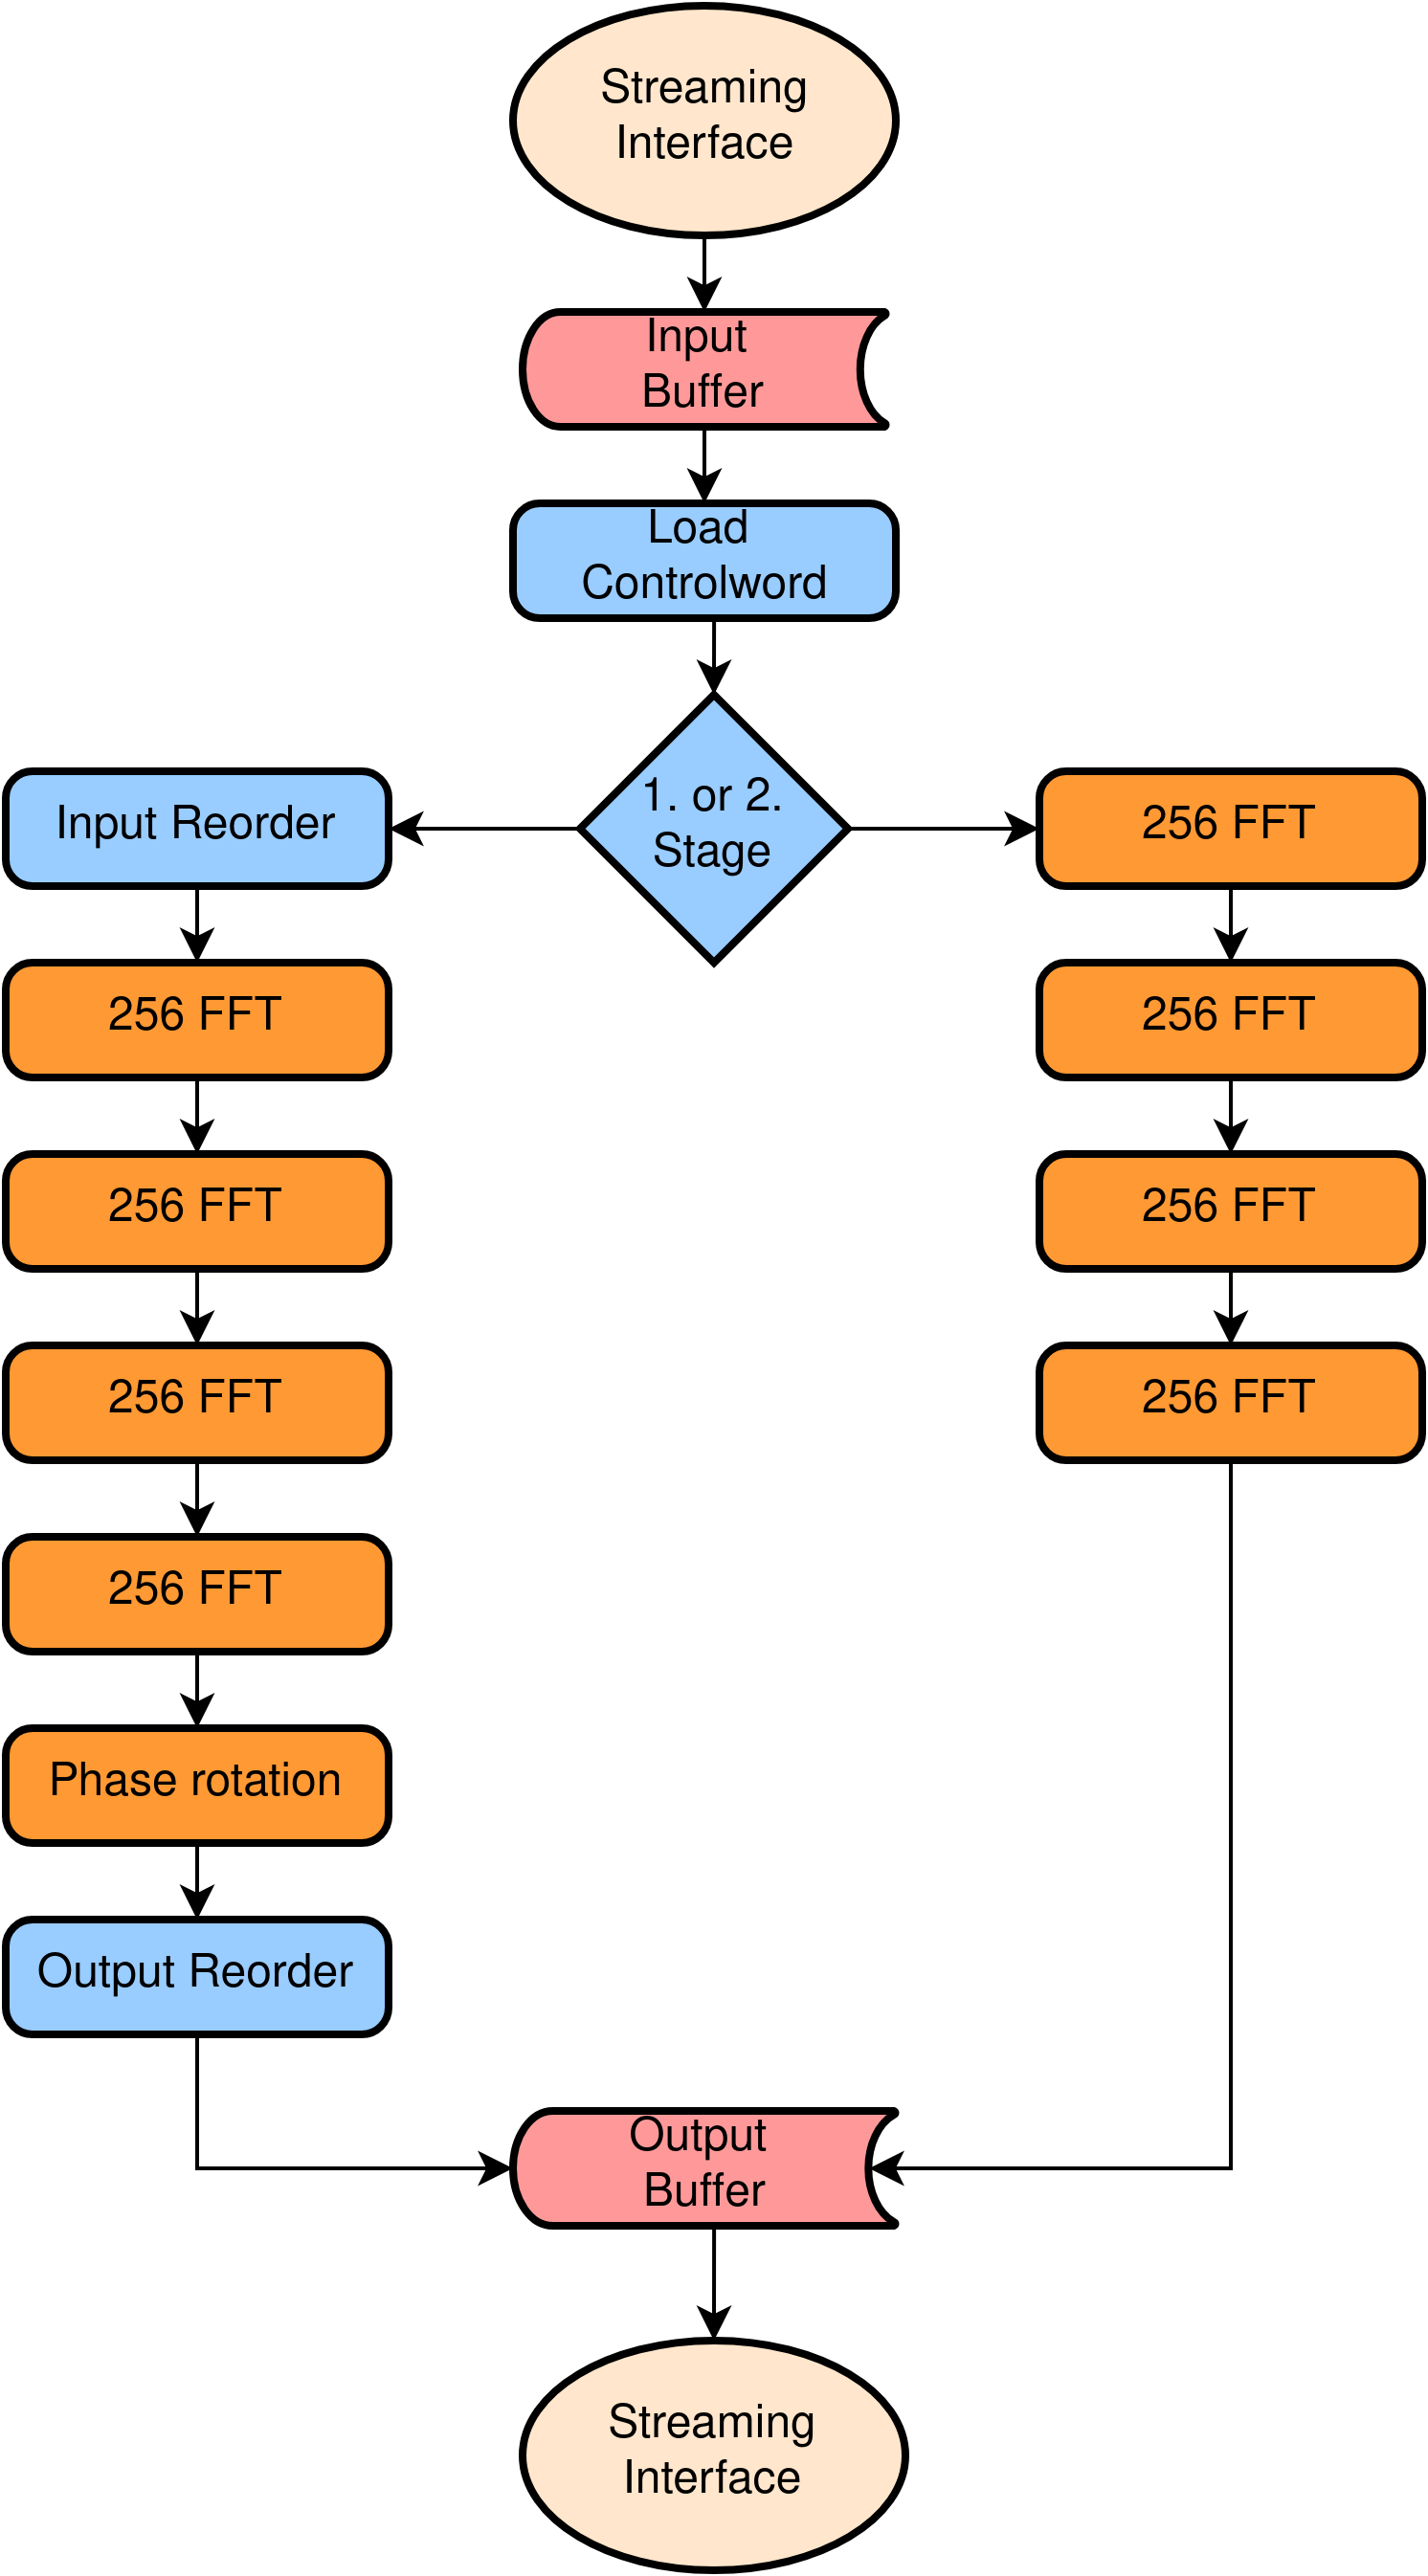
\includegraphics[width=0.45\textwidth]{images/flex_kernel.png}
    \captionsetup{justification=centering}
    \caption{Controlflow of the AI Engine kernel}
        The color in this seem indicate which part of the AI Engine is used for the operation. Red indicates loads and writes to the explicitly allocated memory. Orange are operations that run on the vector unit of the processor. Blue are controlflow functions that do not involve specific calculations. It is shown that both stage need four 256 FFTs. For stage 1 some reorder preparations needed to be done.
    \label{fig:flex_kernel}
\end{figure}

\section{AI Engine kernels}\label{sec:design_ai}
The AI engine kernel is the core component of this algorithm, responsible for the main computations, and is instantiated 256 times. As a result, the kernel must be rigorously optimized to ensure that its runtime remains below the instruction threshold of 73,125,000 instructions per kernel. To achieve this, the kernel heavily utilizes the vector unit of the small \ac{risc} processor. Additionally, the kernel must be adaptable for either a 1024-point \ac{fft} followed by a phase rotation or a set of four independent 256-point \ac{fft}s. Before going into the optimizations of the \ac{fft}s an important point to consider is the handling of the incoming data. The data can either be read element by element from a stream or can be directly copied into the AI Engines memory. For this the design the latter approach is chosen as it reduces the active managed instructions to one, which accepts the dataframe. So at the begin of the kernel the data for the \ac{fft} lies in an buffer. This is shown in figure \ref{fig:flex_kernel} as a red buffer, which is directly filled by the streaming interface.\par
An efficient approach is to split the 1024-point \ac{fft} using the Cooley-Tukey algorithm into four 256-point \ac{fft}s, which are then connected to 256 four-point \ac{fft}s. This strategy enables reuse of the 256-point \ac{fft} in both stages of the algorithm. The distinctions between the two stages are illustrated in Fig. B. As shown, the primary operation of the kernel is the 256-point \ac{fft}, which is invoked multiple times in both variants. Consequently, the next section will examine the design of this component in detail, as its optimization will impact other parts of the kernel as well.\par

\begin{figure}[h]
    \centering
    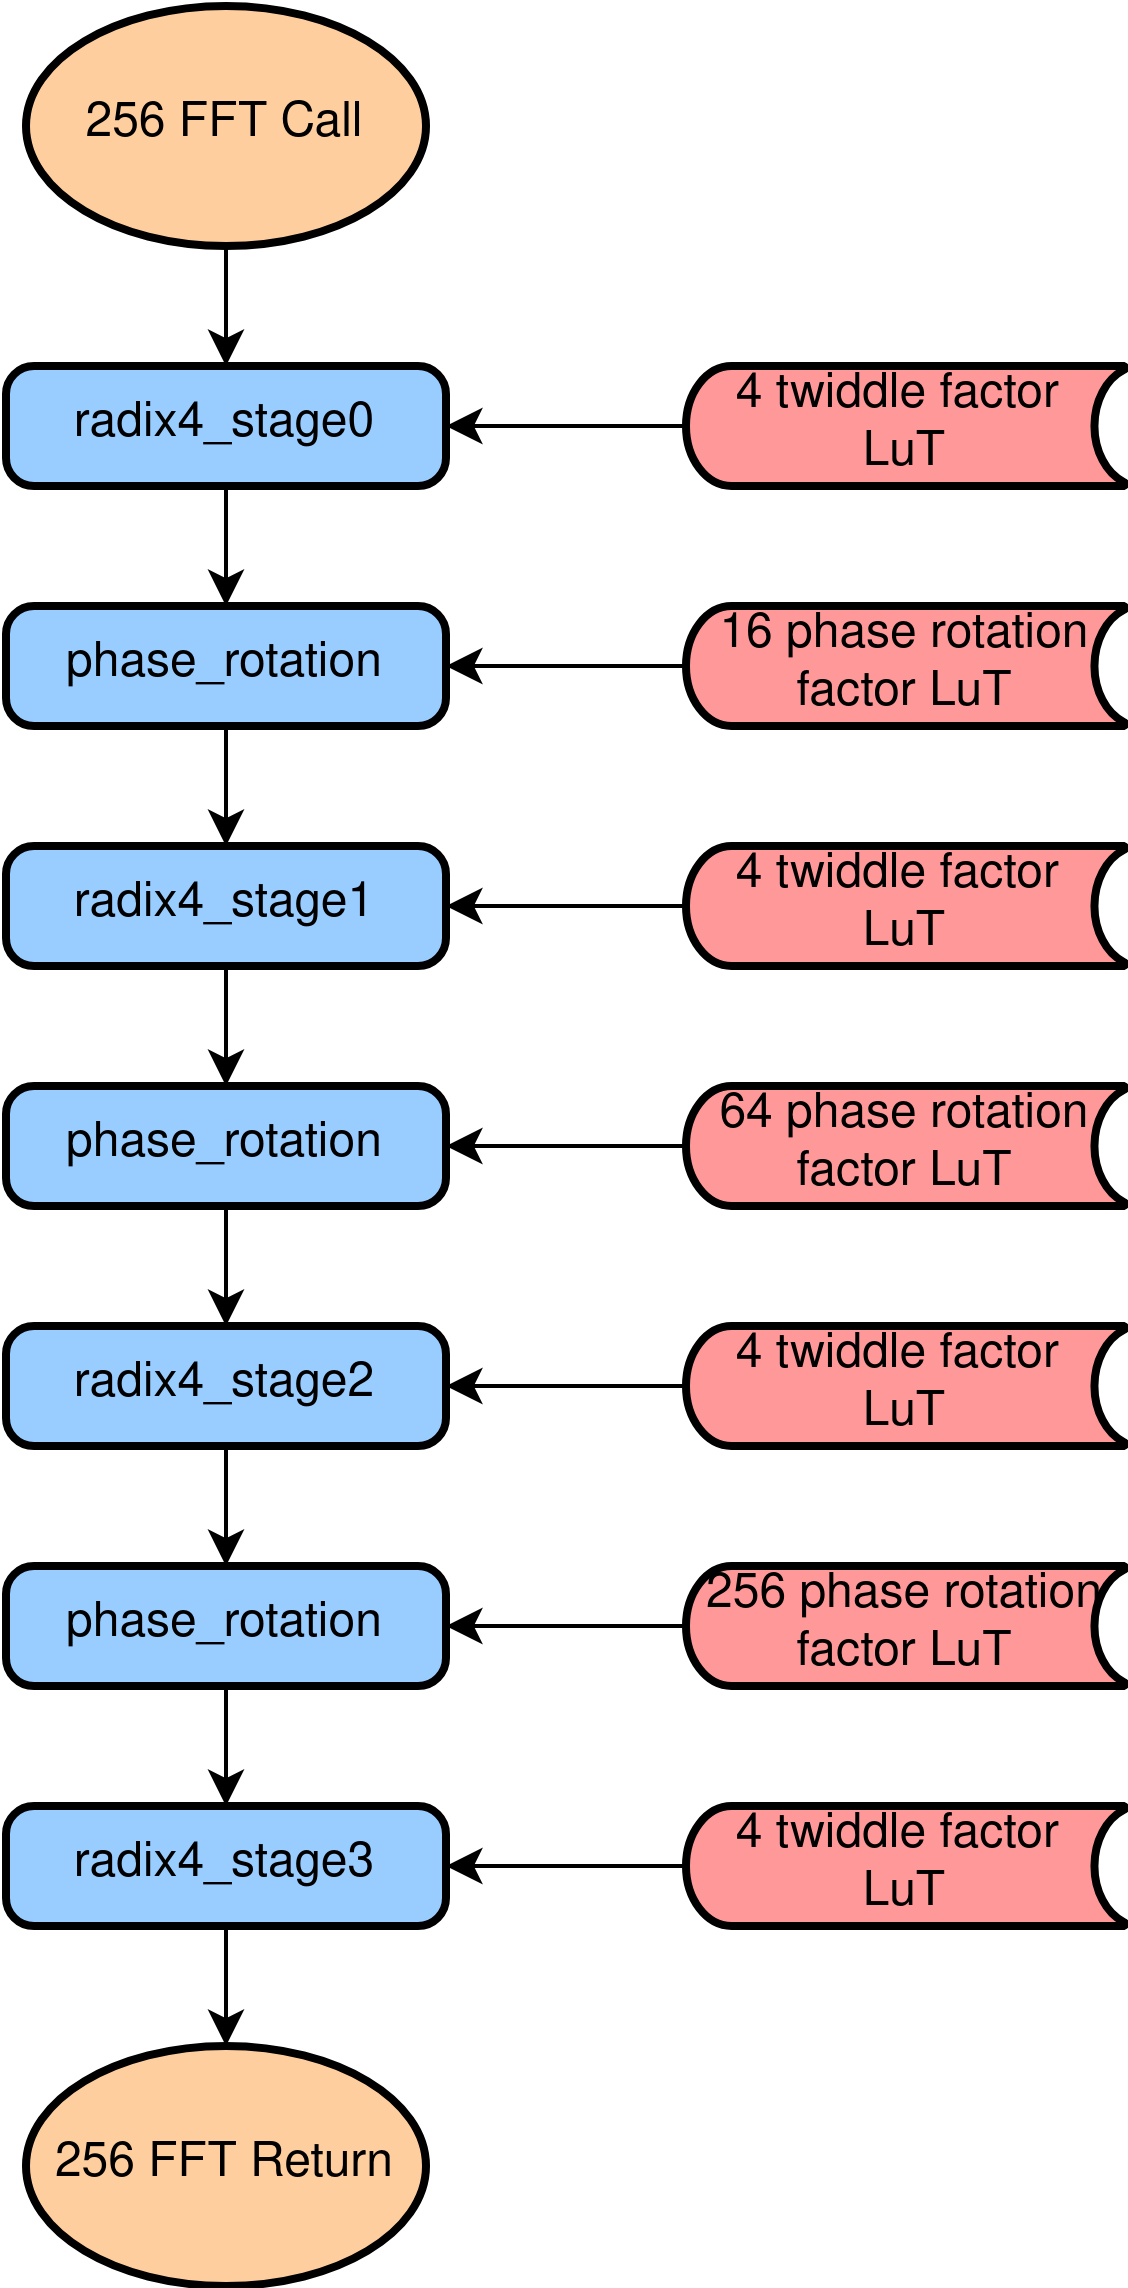
\includegraphics[width=0.35\textwidth]{images/256_func.png}
    \captionsetup{justification=centering}
    \caption{Controlflow of the 256 point \ac{fft}}
            Shows the internal structure of the 256 point FFT with access to special units denoted by color. Red highlights memory operation while orange indicates operations on the vector unit.
    \label{fig:256_kernel}
\end{figure}

The initial step in optimization is the application of the Cooley-Tukey algorithm, which not only facilitates parallelization but also reduces computational complexity, as discussed in section \ref{sec:ft}. This raises the question of the optimal decomposition approach. The decomposition should align with the capabilities of the AI Engine's vector unit. As outlined in section \ref{sec:versal}, the vector unit can perform MAC operations on two vectors of four elements in two instruction cycles. By utilizing twiddle factors in one vector and input values in the other, the smallest feasible \ac{fft} size would be four elements. Therefore, a radix-4 decomposition is the most efficient approach, where the entire 256-point \ac{fft} is constructed from 4-point \ac{fft}s. This process splits the 256-point \ac{fft} into four stages, as illustrated in Fig. C. To achieve this structure, the 256-point \ac{fft} is first divided into four 64-point transformations, each connected to 4-point \ac{fft}s. Each 64-point \ac{fft} is further decomposed into four 16-point \ac{fft}s, which are then split into four 4-point units. The 4-point unit is the smallest computational block, processing two vectors: one containing the input values and the other one containing the twiddle factors, which remain constant for all radix-4 calculations. Between stages, phase rotations are applied to the outputs of the preceding stage with a vectored multiply operation which can also take up to 4 values. To optimize runtime, I have used precalculated twiddle factors and phase rotations. Calculating the twiddle factors during runtime was considered but was overthrown as it would take to much out of the available runtime budget. This results in a total of 596 precalculated values, distributed across 4 twiddle factors, 16 phase rotation factors for the first stage, 64 for the second stage, 256 for the third stage, and 256 for the final stage. Memory savings are achieved in the last stage by exploiting periodicities in the precalculated values.\par
As previously discussed, when calculating four 256-point \ac{fft}s, the routine is invoked four times with different input values, and the results are subsequently streamed to the output. However, additional steps are required when performing a 1024-point \ac{fft} followed by a phase shift. Initially, the data must be reordered. After completing the smaller transforms, the results are multiplied by the phase rotation factors within the 1024-point \ac{fft}, and the 256 four-point \ac{fft}s are applied to the outputs. Finally, the results are multiplied by the precalculated phase rotation factor for the encompassing $2^{18}$-point \ac{fft}. For the initial reordering, the incoming data is partitioned into four blocks, with every fourth element from the unordered data assigned to the same block. After performing the smaller \ac{fft}s on the reordered data, the phase rotation is applied using the precalculated values, similar to the phase rotation between stages of the 256-point \ac{fft}. Following this multiplication, a four-point unit processes the results to connect them. The outputs are then index-reversed, reordered, and multiplied by the 1024-point phase rotation. Like the other phase rotation factors, the values for the 1024-point rotation are also precalculated. Since these factors do not exhibit periodicities, the entire 1024-value table must be stored. Additionally, this table is unique for each instantiation of the AI engine kernel, in contrast to the other lookup tables.
\chapter{Implementation}\label{ch:implementation}
%The purpose of this chapter is, on the one hand, to make it credible that you are not dealing with a "paper tiger" but with a real existing system. It is certainly also a very important text for someone who will continue the work later. The third aspect is to give the reader a deeper impression of the technology that is being dealt with here. Nice examples are "War Stories", i.e. things you had to struggle with in particular. (5-20 pages)

In the following sections, I will demonstrate the implementation of the described design on the Versal platform. The use of the Xilinx toolchain and the general workflow will be outlined. Additionally, the development and implementation of test cases will be discussed, including the generation of test data for these cases.

\section{Implementation on the Versal}\label{sec:imp}
Before delving into the specifics of the implementation, an overview of the Xilinx toolchain is necessary to understand how certain implementation decisions are shaped by the build process. The toolchain primarily consists of the Xilinx v++ compiler and linker \cite{churiwala_designing_2017}. The compiler is used to compile code for the AI engines and to generate the hardware description for the \ac{pl} via high-level synthesis. This process is completed in two steps: first, generating a VHDL file from a C++ design description, and second, compiling this VHDL representation into a .xo hardware file. This approach enables potential VHDL-level optimizations without requiring the design to be rewritten entirely from scratch. The v++ linker then connects and links the AI engine binary with the \ac{pl} description into a single .xsa container file, which can be loaded onto the Versal platform to configure both the \ac{pl} and AI engines. Command-line tools are used to interact with these processes, which can be integrated into a makefile to manage the build sequence. This setup allows for a modularized build process and provides the ability to examine the effects of specific compile flags at each stage.\par
In addition to creating the hardware description container, an application is required to invoke the configured hardware. This application can either be implemented as a bare-metal application or a Linux user-space application. For the latter, a Linux installation on the ARM host system and a compatible compiler are necessary. Implementing the application on Linux is advantageous because it enables the use of existing infrastructure, such as drivers, for interaction with the hardware container. The Linux build system, YOCTO, is employed to acquire the Linux image and set up the configured compiler. YOCTO facilitates the creation of an image and a cross-compiler toolchain with all essential packages and headers \cite{streif_embedded_2016}. In this project, a Linux image and a compiler with the Asio C++ library for networking, generated by YOCTO, are utilized.\par
Once all components are created, they are combined into a single image that can be deployed to the Versal platform. This package is generated by the v++ linker and can include additional files, which will be transferred to the board's memory. This feature is particularly useful for transferring data files to the test environment.

\subsection{Integration of the AI Engine kernel} \label{sec:aie_im}
As previously mentioned, the kernel is implemented in C++ using the Xilinx-specific compiler. Before detailing the complete kernel implementation, I will first describe the implementation of the 256-point \ac{fft}, as it serves as the core functionality of the kernel. The 256-point \ac{fft} is structured as a simple, non-inlined function. This decision stems from the limited program memory available on a single AI Engine tile. However, to reduce function call overhead, all functions within the \ac{fft} are inlined. This approach results in a single code block containing the complete \ac{fft}, which can be entered and exited with one \texttt{jmp} instruction. Consequently, the \ac{fft} function is named \texttt{not\char`_inline\char`_256\char`_FFT}.\par
Within this function, there are multiple calls to different implementations of a function called \texttt{radix\char`_4\char`_stage}. They range from zero to three, representing the four \ac{fft} stages described in section \ref{sec:design_ai}. These stages are abstracted into separate functions, enabling flexibility for future modifications, such as adding or removing stages. Each function is similar in structure, with slight variations tailored to each stage. I will first outline the general structure, as it is consistent across each function. Generally, the functions accept four cfloat pointers as input: two pointing to the input and output buffers, and the other two pointing to lookup tables—one for twiddle factors within the \ac{fft} stage and the other for phase rotation. All functions utilize the radix-4 \ac{fft}, so the first lookup table consistently uses the same pointer to the radix-4 lookup table. The general structure of the algorithm is depicted as pseudo-code in \ref{alg:FFT}.\par
The radix-4 \ac{fft} is implemented using the \texttt{fpmac} intrinsic provided by the AI Engine \cite{AMD_aie_intrinsics}. This intrinsic performs a multiply-and-add operation on two input vectors of four elements each within two clock cycles. To implement the four-point \ac{fft}, the \texttt{fpmac} operation is invoked four times, acting on four elements of the input vector and the twiddle factor lookup table. During these calls, the element order for multiplication and addition is adjusted to model the entire \ac{fft}. This approach reduces the \ac{fft} cycle count from 32 cycles (16 for multiplication and 16 for addition) to 8 cycles for the four \texttt{fpmac} calls. Following this, a vector multiplication (\texttt{fpmul}) with the second lookup table is applied to the result vector to complete the phase rotation.\par
For these vector operations, the relevant sections of the buffer and lookup tables must be loaded into the vector registers, as described in section \ref{sec:versal}. Consequently, two load operations are executed before each \texttt{fpmac} and \texttt{fpmul} operation. To minimize loading overhead, the input buffer is divided into four segments, which are loaded into the vector register simultaneously. This creates a loop where four four-element vectors are loaded into the vector register. The \texttt{fpmac} operations for the \ac{fft} are then executed on these preloaded vectors, and phase rotation is subsequently applied to the results. This loop continues until every element of the output buffer has been calculated. For each of the aforementioned \ac{fft} stages, the size of the segmented input buffer and, therefore, the loop iterations vary, which necessitates distinct functions for each stage. The general structure is shown in the following pseudo-code while figure \ref{fig:vector_load} shows the utilization of the vector unit.\par

\begin{algorithm}
\caption{FFT Implementation} \label{alg:FFT}
\begin{footnotesize} % Reduzierte Schriftgröße
\begin{algorithmic}
\STATE \textbf{Function} \textit{not\_inline\_256\_FFT}(input\_buffer, output\_buffer, tw\_lut, ph\_lut)
    \STATE \hspace{0.3cm} \textbf{for each} stage in \{0, 1, 2, 3\} \textbf{do}
    \STATE \hspace{0.6cm} \textit{radix\_4\_stage}(input\_buffer, output\_buffer, tw\_lut, ph\_lut, stage)
    \STATE \hspace{0.3cm} \textbf{end for}
    \STATE \hspace{0.3cm} \textit{reorder\_output}(output\_buffer)
\STATE \textbf{End Function}

\STATE \textbf{Function} \textit{radix\_4\_stage}(input\_buffer, output\_buffer, tw\_lut, ph\_lut, stage)
    \STATE \hspace{0.3cm} \textbf{for each} seg in in\_buf \textbf{do}
    \STATE \hspace{0.6cm} Load seg into vector register
    \STATE \hspace{0.6cm} \textbf{for} i = 1 to 4 \textbf{do}
    \STATE \hspace{0.9cm} Perform \textit{fpmac} with tw\_lut and input vec
    \STATE \hspace{0.6cm} \textbf{end for}
    \STATE \hspace{0.6cm} Perform \textit{fpmul} with ph\_lut for phase rotation
    \STATE \hspace{0.3cm} \textbf{end for}
\STATE \textbf{End Function}

\STATE \textbf{Function} \textit{reorder\_output}(output\_buffer)
    \STATE \hspace{0.3cm} Reorder elements in out\_buf for sequential loading
\STATE \textbf{End Function}
\end{algorithmic}
\end{footnotesize}
\end{algorithm}


\begin{figure}[h]
    \centering
    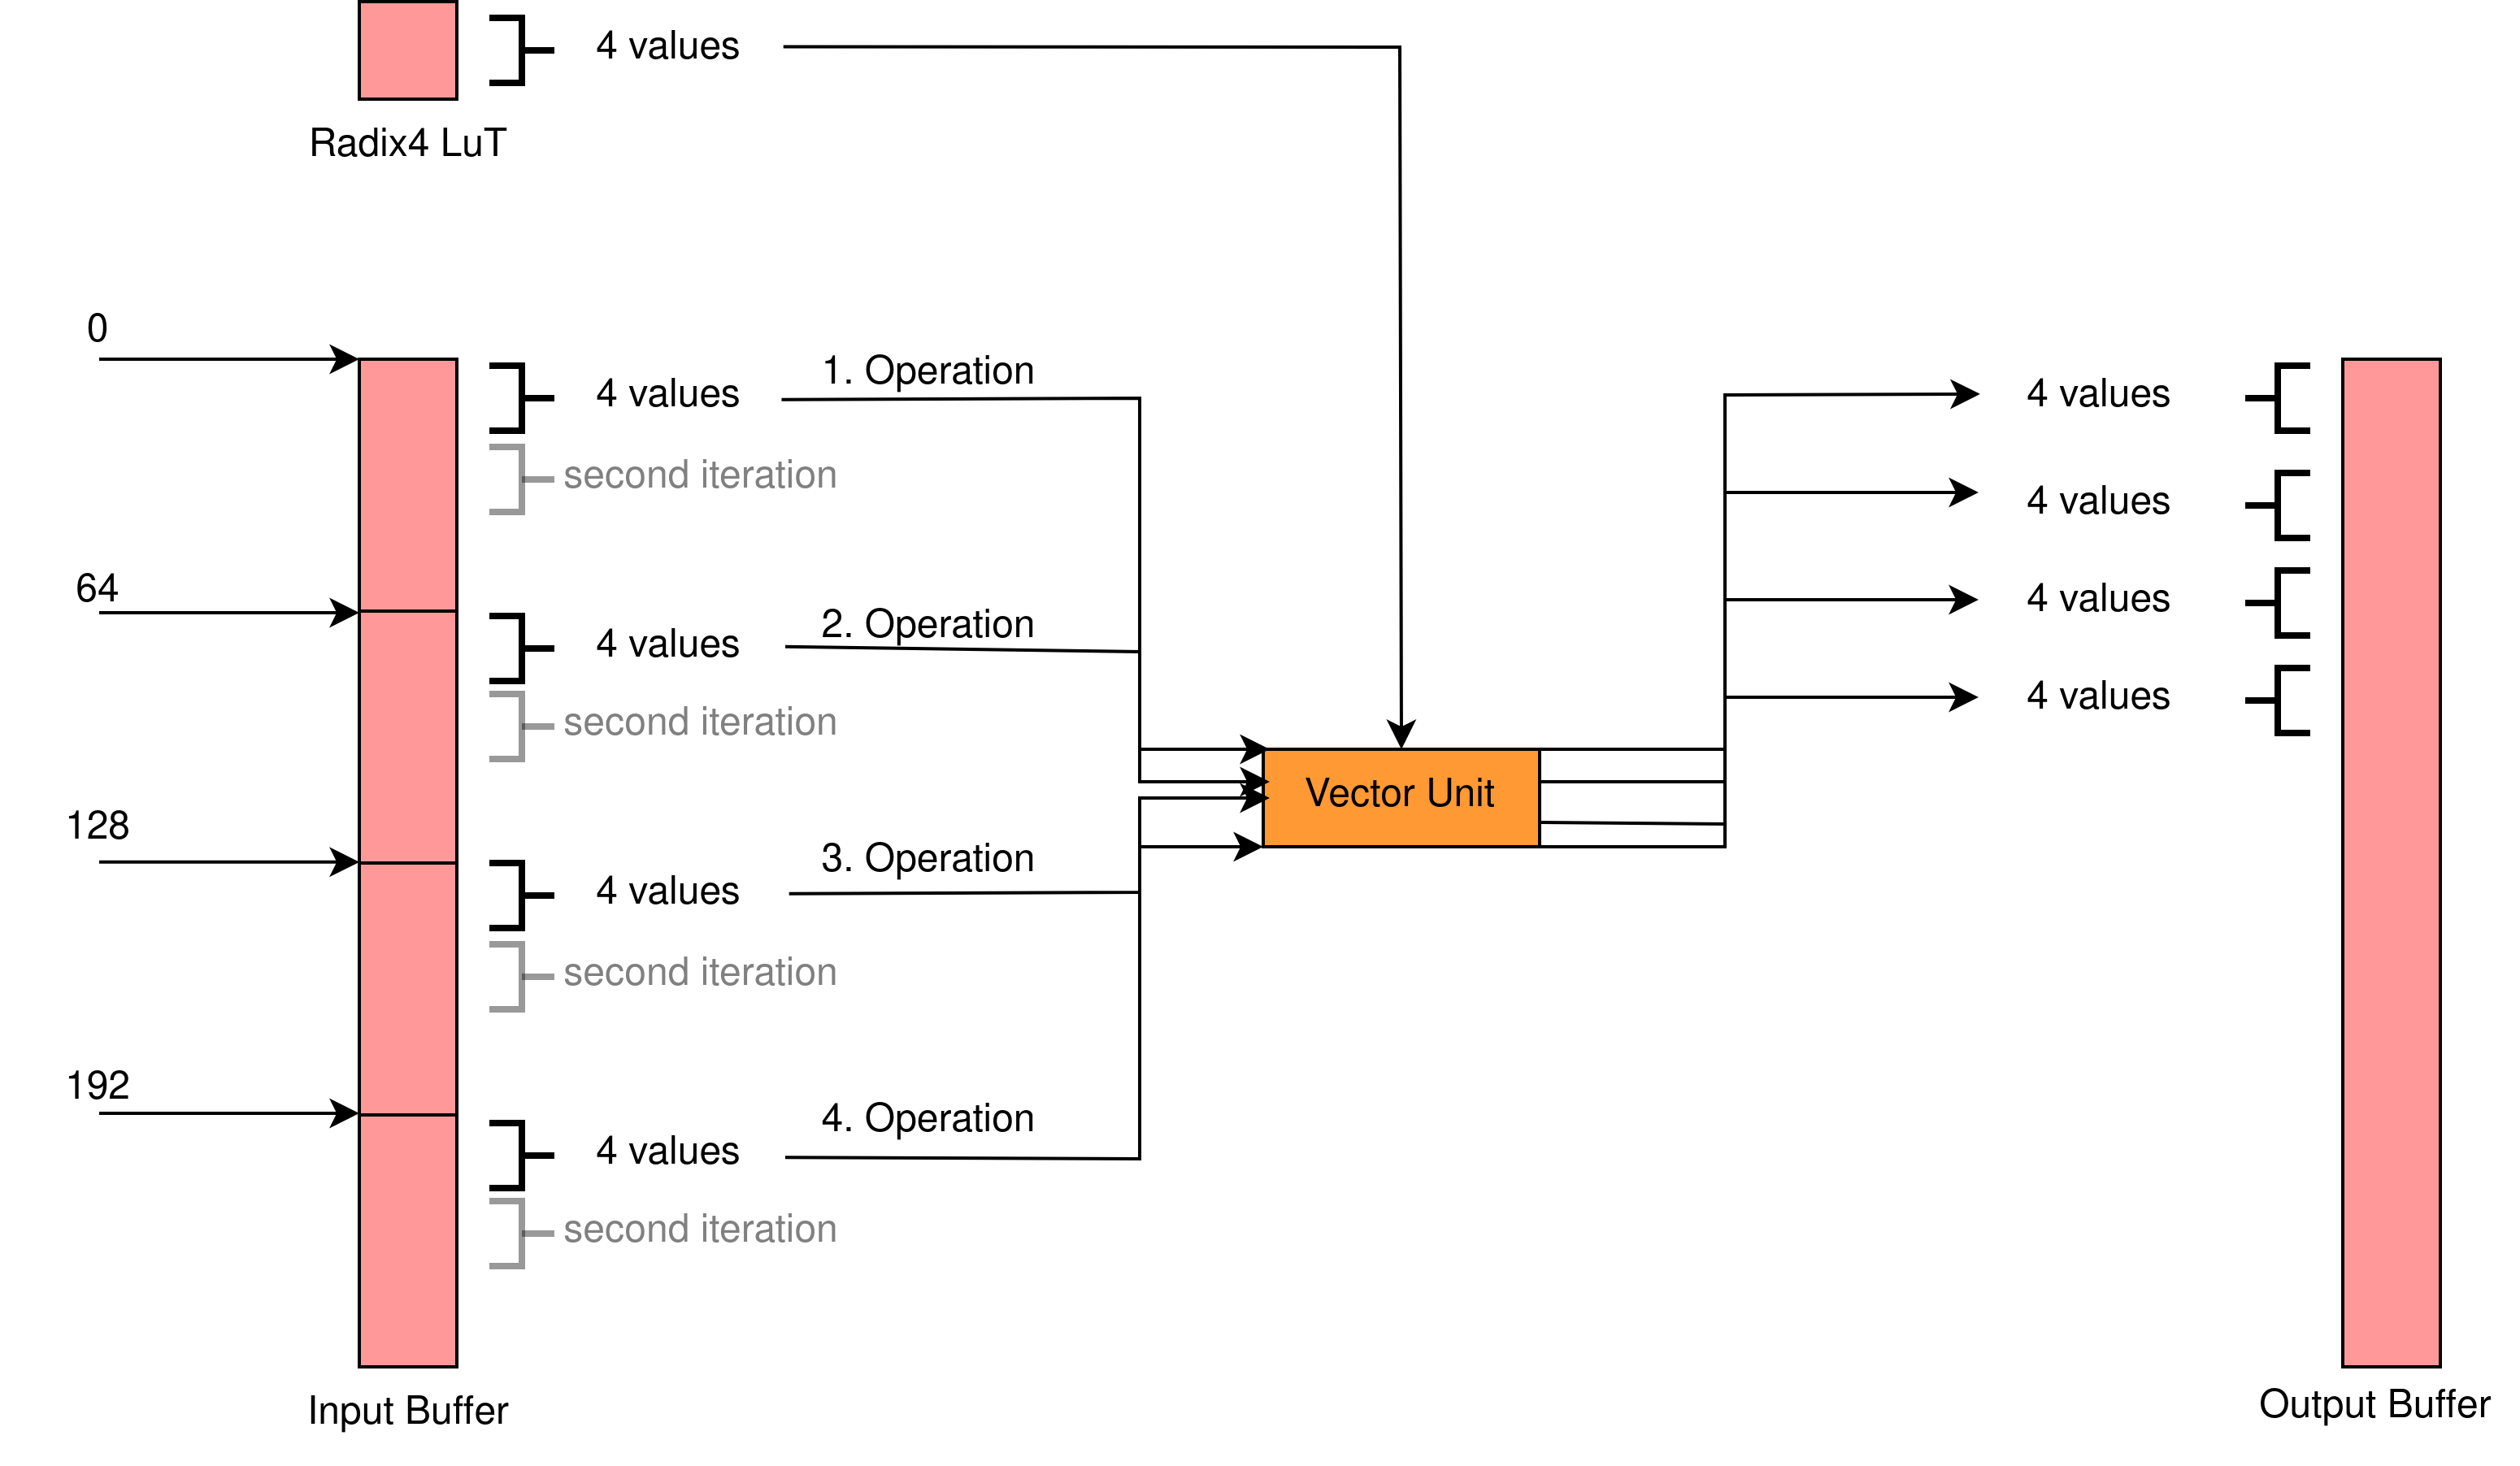
\includegraphics[width=1.0\textwidth]{images/vector_load.png}
    \captionsetup{justification=centering}
    \caption{Load order for the vector unit}
        Memory loads from the memory banks in red to the vector registers in orange during multiple iterations of the radix-4 functions. One load to each 64 value block of the input buffer is done during every iteration. 
    \label{fig:vector_load}
\end{figure}

Between the different \ac{fft} stages, a reorder function is used to enable sequential element loading from the buffer into the vector unit, thereby minimizing and accelerating read and write operations. Like the other functions, these reorder functions are inlined to contribute to the monolithic \texttt{not\char`_inline\char`_256\char`_FFT} code block. \par
Having discussed the construction of the main \ac{fft} function, I will now describe the complete kernel. The kernel function operates on two cfloat buffers, each containing 1024 elements for input and output. Each buffer occupies one memory rank of the AI Engine tile’s buffer. To ensure memory alignment, the control word, which configures the kernel, must also fit within this buffer. A simple yet effective solution is to place this control word within the data frame, as the initial input for the first stage of the $2^{18}$-point \ac{fft} is real-valued, requiring the same buffer as the complex-valued input of the second stage. Therefore, the complex components of the input buffer remain unused. The control word is intentionally designed to be an invalid floating-point value, which the kernel can identify. The kernel operation checks whether the first complex value in the input buffer is NaN. If so, the kernel is set up for the first stage, and the first complex value is reset to zero. If the value is valid, the kernel is set up for the second stage, and no changes are made to the data frame. In both configurations, the \texttt{not\char`_inline\char`_256\char`_FFT}function is called four times on different segments of the data frame. Data frame access is managed through four pointers, each pointing to a different 256-point segment. Intermediate results between \ac{fft} stages are stored in the output buffer, which is only streamed when its final element is written. To avoid filling the output buffer, an additional 256-element buffer is used. If the kernel is configured for the first stage, a phase rotation is applied afterward using the \texttt{fpmul} operation described earlier. Each kernel instance has a unique phase rotation lookup table, assigned through preprocessor directives. The complete kernel is generated as a macro, invoked before compilation to create kernel functions with distinct lookup tables.\par
To define the data paths between kernels, a directed graph is used, as outlined in section \ref{sec:versal}. Each class capable of sending or receiving data includes input, output, or both types of ports, which can be connected to represent directed data streams. Thus, only output-to-input connections are valid. The kernel function described above is instantiated within a kernel class, which calls this function internally. The size of the input buffer dictates the number of elements that must be streamed to the input port before invoking this function, which, in this case, requires exactly 1024 elements. Failure to stream this quantity will result in a system crash. The general memory utilization is shown in figure \ref{fig:memory_structure}. \par
For this design, multiple input streams are defined and exposed to the \ac{pl}. This is achieved using the \texttt{input\char`_plio} and \texttt{output\char`_plio} classes, which serve as abstractions for connection tiles. The \texttt{pktsplit} class is used to divide the eight input streams into 32 data packets, mimicking the routing hardware's split mechanism. This class has one input port and a maximum of 32 output ports. Each \texttt{input\char`_plio} output port connects to a \texttt{pktsplit} input port, and each \texttt{pktsplit} output port connects to an individual kernel instance input port. This design employs 256 kernel instances. For the reverse flow, to merge data back into the \ac{pl}, the \texttt{pktmerge} class is used. Acting as the \texttt{pktsplit} counterpart, it accepts 32 inputs and merges them into a single output stream, meaning that 32 kernel instances connect to one \texttt{pktmerge}, which in turn connects to an \texttt{output\char`_plio}. This allows to only use eight of the connection tiles of the AI Engine array. In consequence the \ac{pl} kernel only need to deal with eight streams which reduces the overhead.\par
In addition to the input and output ports, each kernel can also have multiple parameter ports, which can connect to lookup tables. For this design, each kernel includes six parameter ports connected to lookup tables for the different \ac{fft} stages. These lookup tables are defined as arrays and are automatically generated by a Python script. During compile time they are assigned to a memory location within the AI Engine memory block.

\begin{figure}[h]
    \centering
    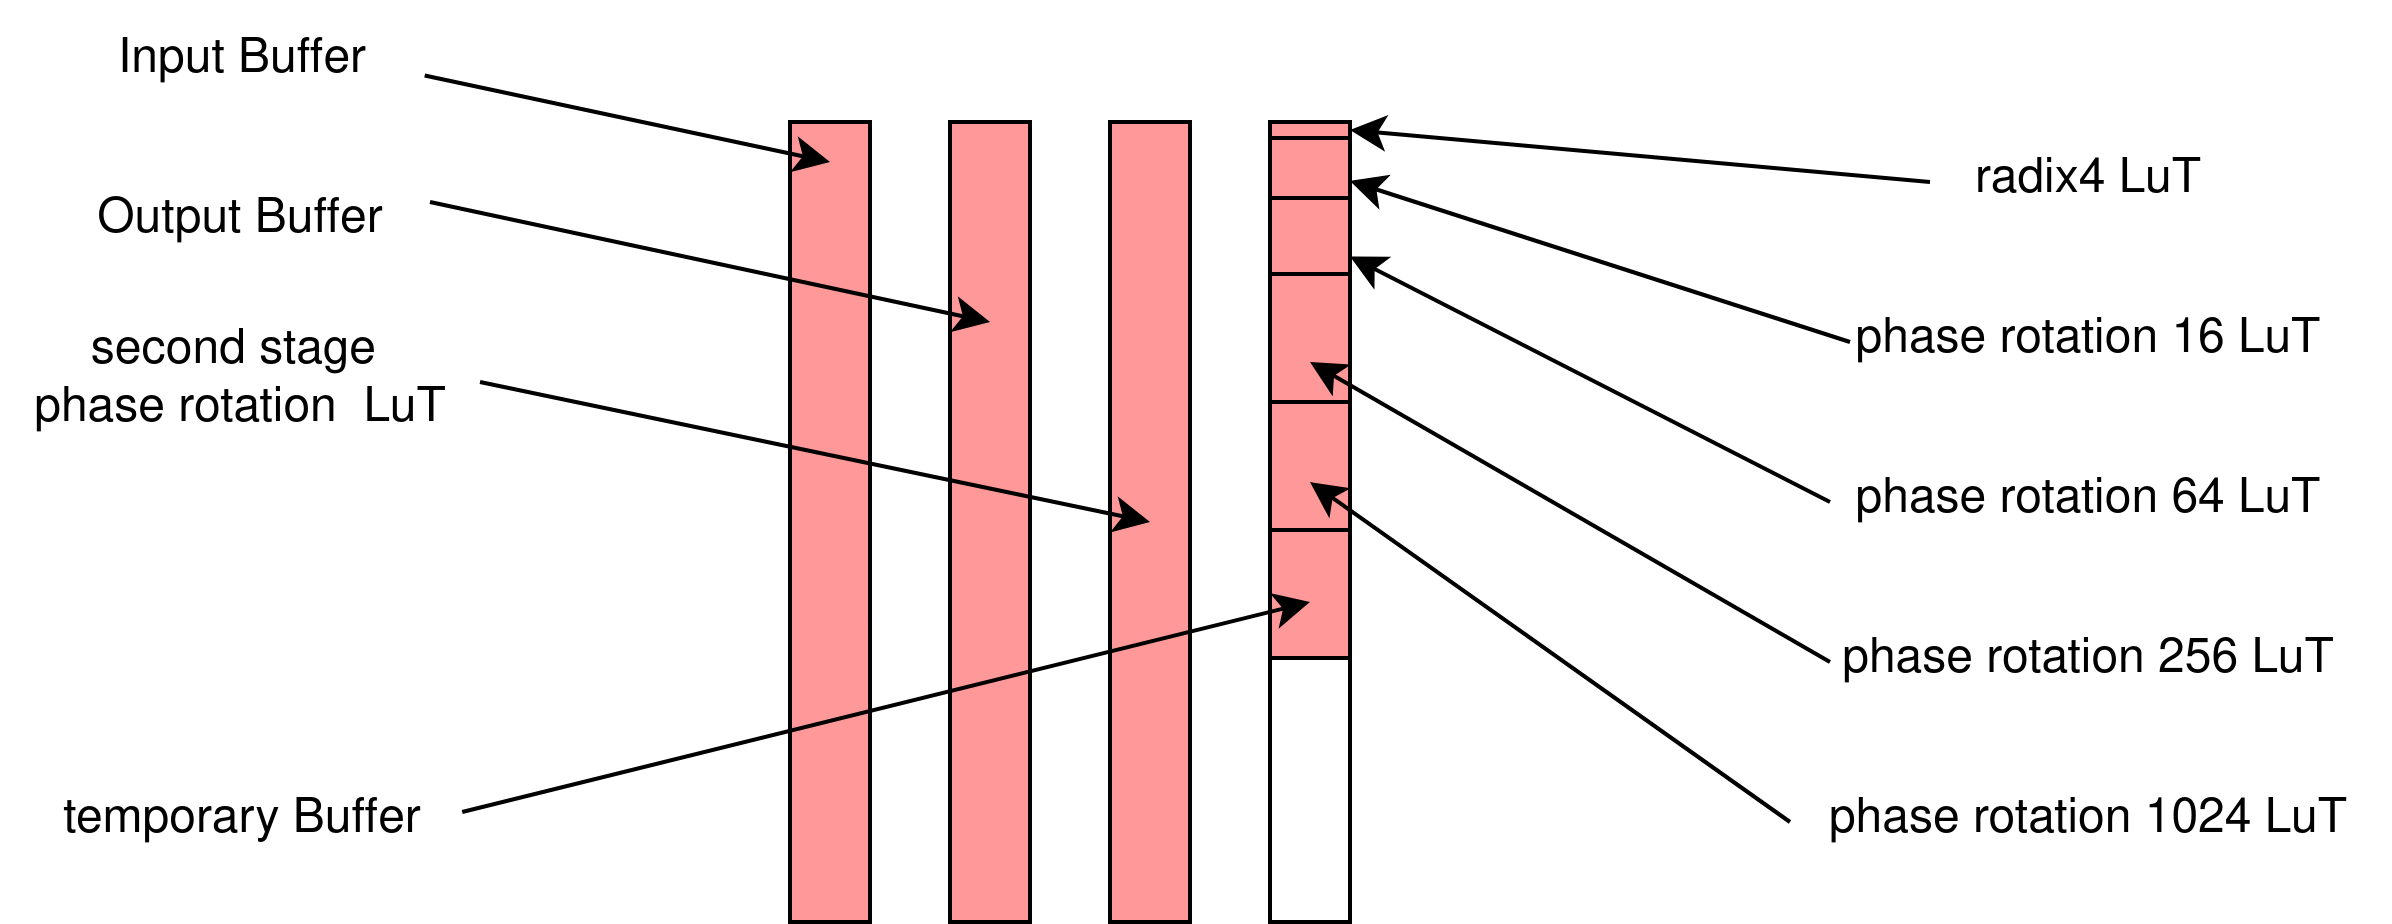
\includegraphics[width=1.0\textwidth]{images/memory_structure.png}
    \captionsetup{justification=centering}
    \caption{Occupied memory banks of the 32 kb AI Engine memory}
        The memory utilization of every single memory bank. Red shows the alocated memory split into its use cases.
    \label{fig:memory_structure}
\end{figure}

\subsection{Construction of the programmable logic}
As previously described, the \ac{pl} is defined using high-level synthesis \cite{coussy_introduction_2009} in C++. Kernels within the \ac{pl} are defined as functions specifying the kernel’s functionality. Consequently, the reorder mechanisms across kernels are implemented as simple loops that write values into an array in the correct order. These values are then read from the array and sequentially streamed between kernels.\par
Several points require special consideration in this setup. First, the use of arrays: unlike in a conventional program, arrays in this context do not lead to RAM memory allocation, as the \ac{pl} lacks such memory. Instead, the array is implemented in \ac{pl} using available block RAM. This allows faster access as the memory is directly connected to the streams and does not have an virtualisation layer between these two components. On the other hand it necessitates careful considerations regarding the size of certain buffers as memory can not be allocated or swapped out easily. The current design lead to an allocation of 63 percent of the available block RAM resources and 27 percent allocation of the available LuT resources.  Another essential point is the handling of streams between \ac{pl} kernels and between these kernels and the AI Engines. Streams between kernels are initiated as arguments in the function defining a kernel. For this implementation, AXI streams are used, as they also provide compatibility with the AI Engines without requiring protocol modifications. Xilinx's AXI implementation offers both blocking and non-blocking read and write operations for streams. With blocking reads, writes are only executed once reads from all streams are completed. This could pose an issue for the design, specifically in a kernel with multiple input streams, where not all streams are active simultaneously. For example, the Packetsender kernel can receive streams from either the Partitioner or the Reorderer. To accommodate this, it includes eight streams connected to the Partitioner and eight connected to the Reorderer. A blocking read would delay all writes until data from all 16 streams is read. To avoid this, the non-blocking variant is used, allowing synchronization concerns to be managed by buffering data in an array beforehand.\par
The methods chosen to implement \ac{pl} kernels enable a straightforward and efficient design, allowing more focus on the overall structure and the AI Engines, which are the primary focus of this work.\par

\subsection{Host application}
The host application runs on the ARM processor and manages both the AI Engines and the \ac{pl}. From the host application’s perspective, the \ac{pl} and AI Engines act as accelerators to which tasks can be delegated, following a target-offloading approach. The application runs in userspace on a Linux operating system, enabling userspace drivers to interact with the hardware as shown in figure \ref{fig:host_interact}. Xilinx provides the Xilinx Runtime (XRT) \cite{xrt}, a user-kernel driver combination, to facilitate this interaction. One of XRT’s key functions is loading a hardware container, which is the linked result of the AI Engine and \ac{pl} kernels, and configures the hardware with the programmed functionality. The XRT’s load function flashes this container onto the hardware.\par
Once configured, the AI Engines and \ac{pl} functionalities are called using different methods. For \ac{pl} kernels that interact with DDR memory, memory must be allocated and passed to the kernel. The kernel can then be activated by calling it as a function, after which it starts running as soon as data is written to its memory location. Other \ac{pl} kernels operate similarly, starting execution upon receiving data from a stream. The AI Engine graph, however, is instantiated as a class with various callable functions. The graph is initialized with \texttt{graph.init()} and started with \texttt{graph.run()}. Like the \ac{pl} kernels, the AI Engines begin execution when data is streamed to the connection tiles. The \texttt{run()} function accepts an argument specifying the number of graph run repetitions. For example, passing \texttt{1} means the graph will execute once, and if data continues to stream afterward, the engines will stall. In this design, two calls to the AI Engines are made, one for the first \ac{fft} stage and one for the second, so \texttt{graph.run(2)} is used. Upon completing both runs, resources are released with \texttt{graph.end()}.\par
With the management of \ac{pl} and AI Engines from the host application described, an overview of data loading and result processing is provided here. The algorithm’s input data is initially read from a text file and copied to memory allocated for the Partitioner. After execution, results are retrieved from memory allocated for the Collector and saved to an output file. These results are used to calculate the root mean square error (RMSE) by comparing them to precomputed correct values from another file. All of these steps take place locally on the Versal platform. To transfer results to another system for further analysis, a network connection is established using the Asio C++ library. The following section will delve into the generation of test data and the computation of the correct results used as the ground truth.\par

\begin{figure}[h]
    \centering
    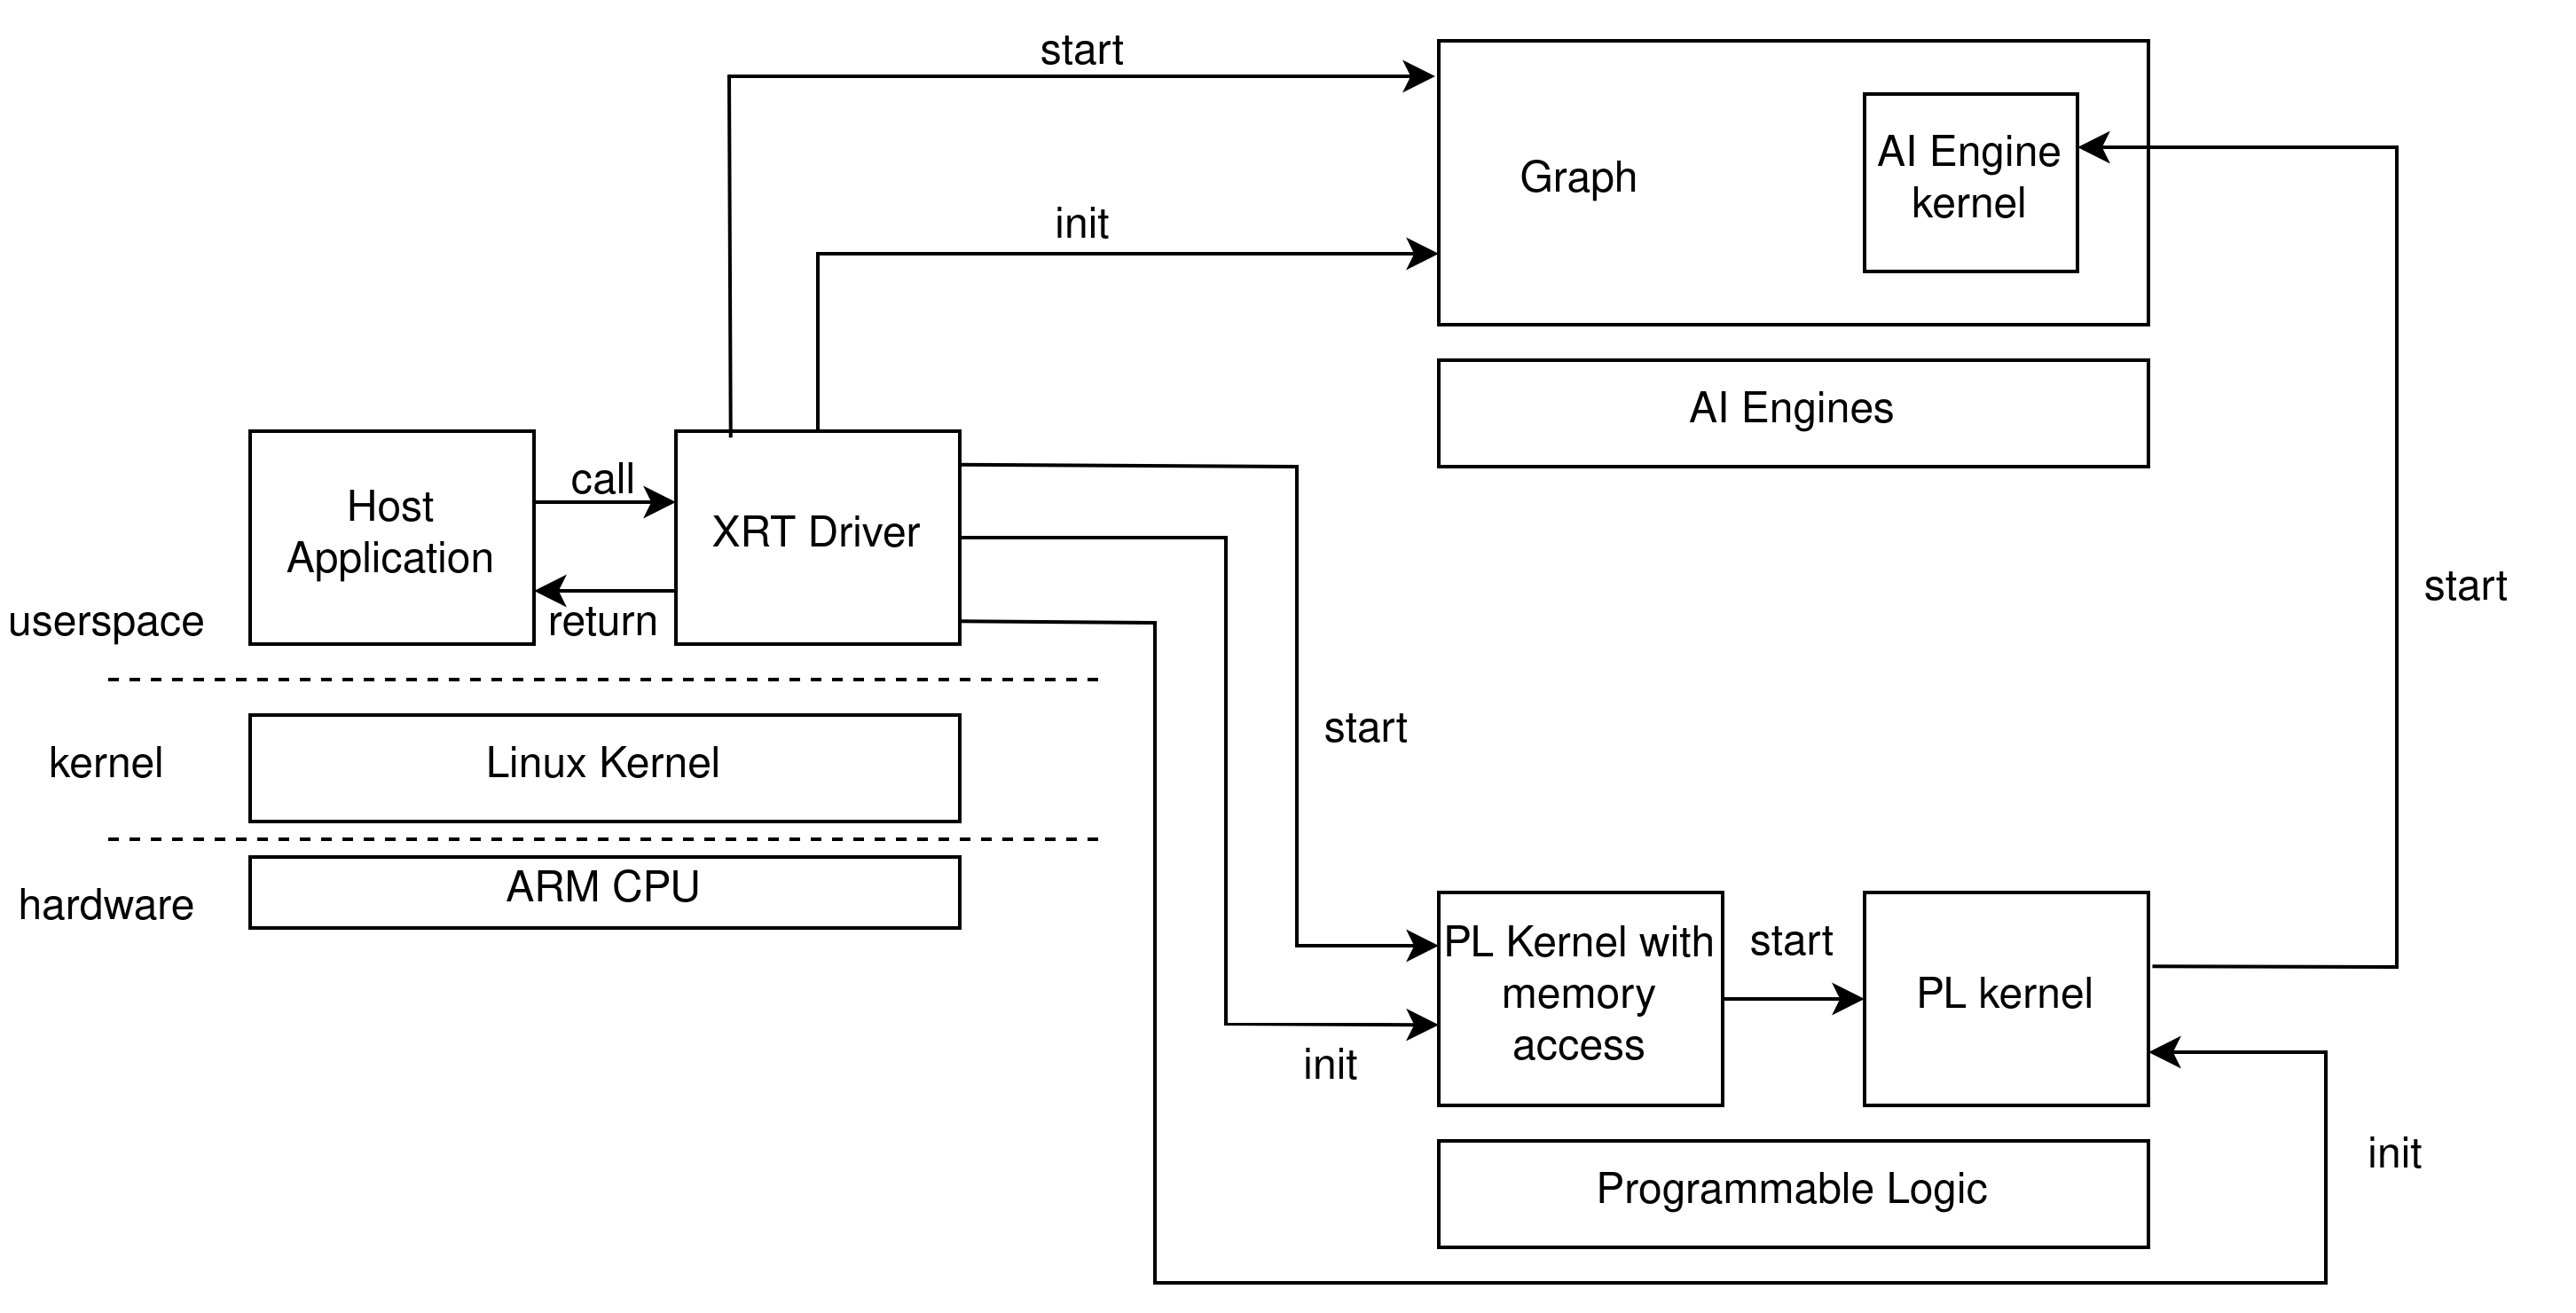
\includegraphics[width=1.0\textwidth]{images/host_interaction.png}
    \captionsetup{justification=centering}
    \caption{XRT Driver interaction scheme}
        This schematic shows the interaction of the host application with the XRT driver which enables the program flashed onto the PL and the AI Engines. Some specific functions are started from within the PL but are still initialised by the XRT driver.
    \label{fig:host_interact}
\end{figure}

%TODO add source for FFTW3, mersenne twister etc.
\section{Test data generation}
The generation of test data consists of two main parts: generating the real-valued input data and computing the expected results. For the input data generation, certain requirements must be met. The data should be randomly structured to avoid patterns that could favor a specific \ac{fft} algorithm. Although the data is random, it must also be reproducible to ensure comparability across tests. To achieve this, a random seed is generated using the \texttt{std::random\char`_device\char`_rd} function from the standard C++ library. This seed is stored to enable the generation of the same input data in future runs. The seed initializes the Mersenne Twister algorithm \texttt{std::mt19937}, an efficient pseudo-random number generator in C++ \cite{matsumoto_mersenne_1998}. This generator creates a consistent sequence of random numbers for a given seed. Each random number is transformed into a floating-point value between 0 and 100 using \texttt{std::uniform\char`_real\char`_distribution<float> dis(0, 100)}. These bounds are arbitrary and can be adjusted for different test cases. Each generated value is stored in a file, and a zero is added between each value to serve as the imaginary part, which is zero for a real-valued signal.\par
This file is then used to generate ground truth data by performing an \ac{fft} on it, which is done on an x86 \ac{cpu} using the FFTW3 library for C++. FFTW3 is a highly optimized library for fast \ac{fft} implementations across multiple platforms \cite{frigo_design_2005}, making it an ideal choice for generating this test case.\par
All generated data files are included in the package that is flashed onto the SD card, allowing them to be accessed directly on the Versal platform. 

\chapter{Evaluation}\label{ch:eval}
%Every job in our field includes a performance evaluation. This chapter should show which methods have been used to evaluate performance and what results have been achieved. It is important not only to provide the reader with some figures, but also to discuss the results. It is very good if you first discuss and make plausible what results you expect and then discuss possible deviations. (up to 10 pages)

The design was evaluated in multiple steps to assess the impact of specific design decisions. To expedite the testing cycle, a smaller prototype comprising only 32,768 units was utilized, reducing the compilation time from over 10 hours to approximately 45 minutes. This smaller prototype employs the same techniques as the larger design, but it is decomposed into 256- and 128-point kernels. The evaluation focused on both runtime and precision metrics. For an accurate analysis, the runtime was measured separately for the \ac{pl} and the AI Engines. Given that the primary focus of this work is on the AI Engines, they are expected to perform significantly better than the \ac{pl}.\par

%TODO change name to test case or something else more appropriate
\section{Benchmark setup}
For the aforementioned analysis, various measurements are required. These measurements are conducted using the XRT driver described in section \ref{sec:aie_im}. The start and stop points of the measurements are illustrated in figure \ref{fig:timing}. As shown, all measurements commence and conclude either before or after data is written to the main memory. This approach is taken because the DDR access times are not considered part of the algorithm. In practice, the data is expected to originate from one of the various I/O streaming ports and will be sent there for further processing. The \ac{cpu} and DDR are not involved in this process. Additionally, it is important to note that each component of the algorithm is measured separately, and one comprehensive measurement is performed for a complete run of all components. To ensure reliable results, each measurement is repeated 10 times, and the mean value of the results is calculated.\par

\begin{figure}[h]
    \centering
    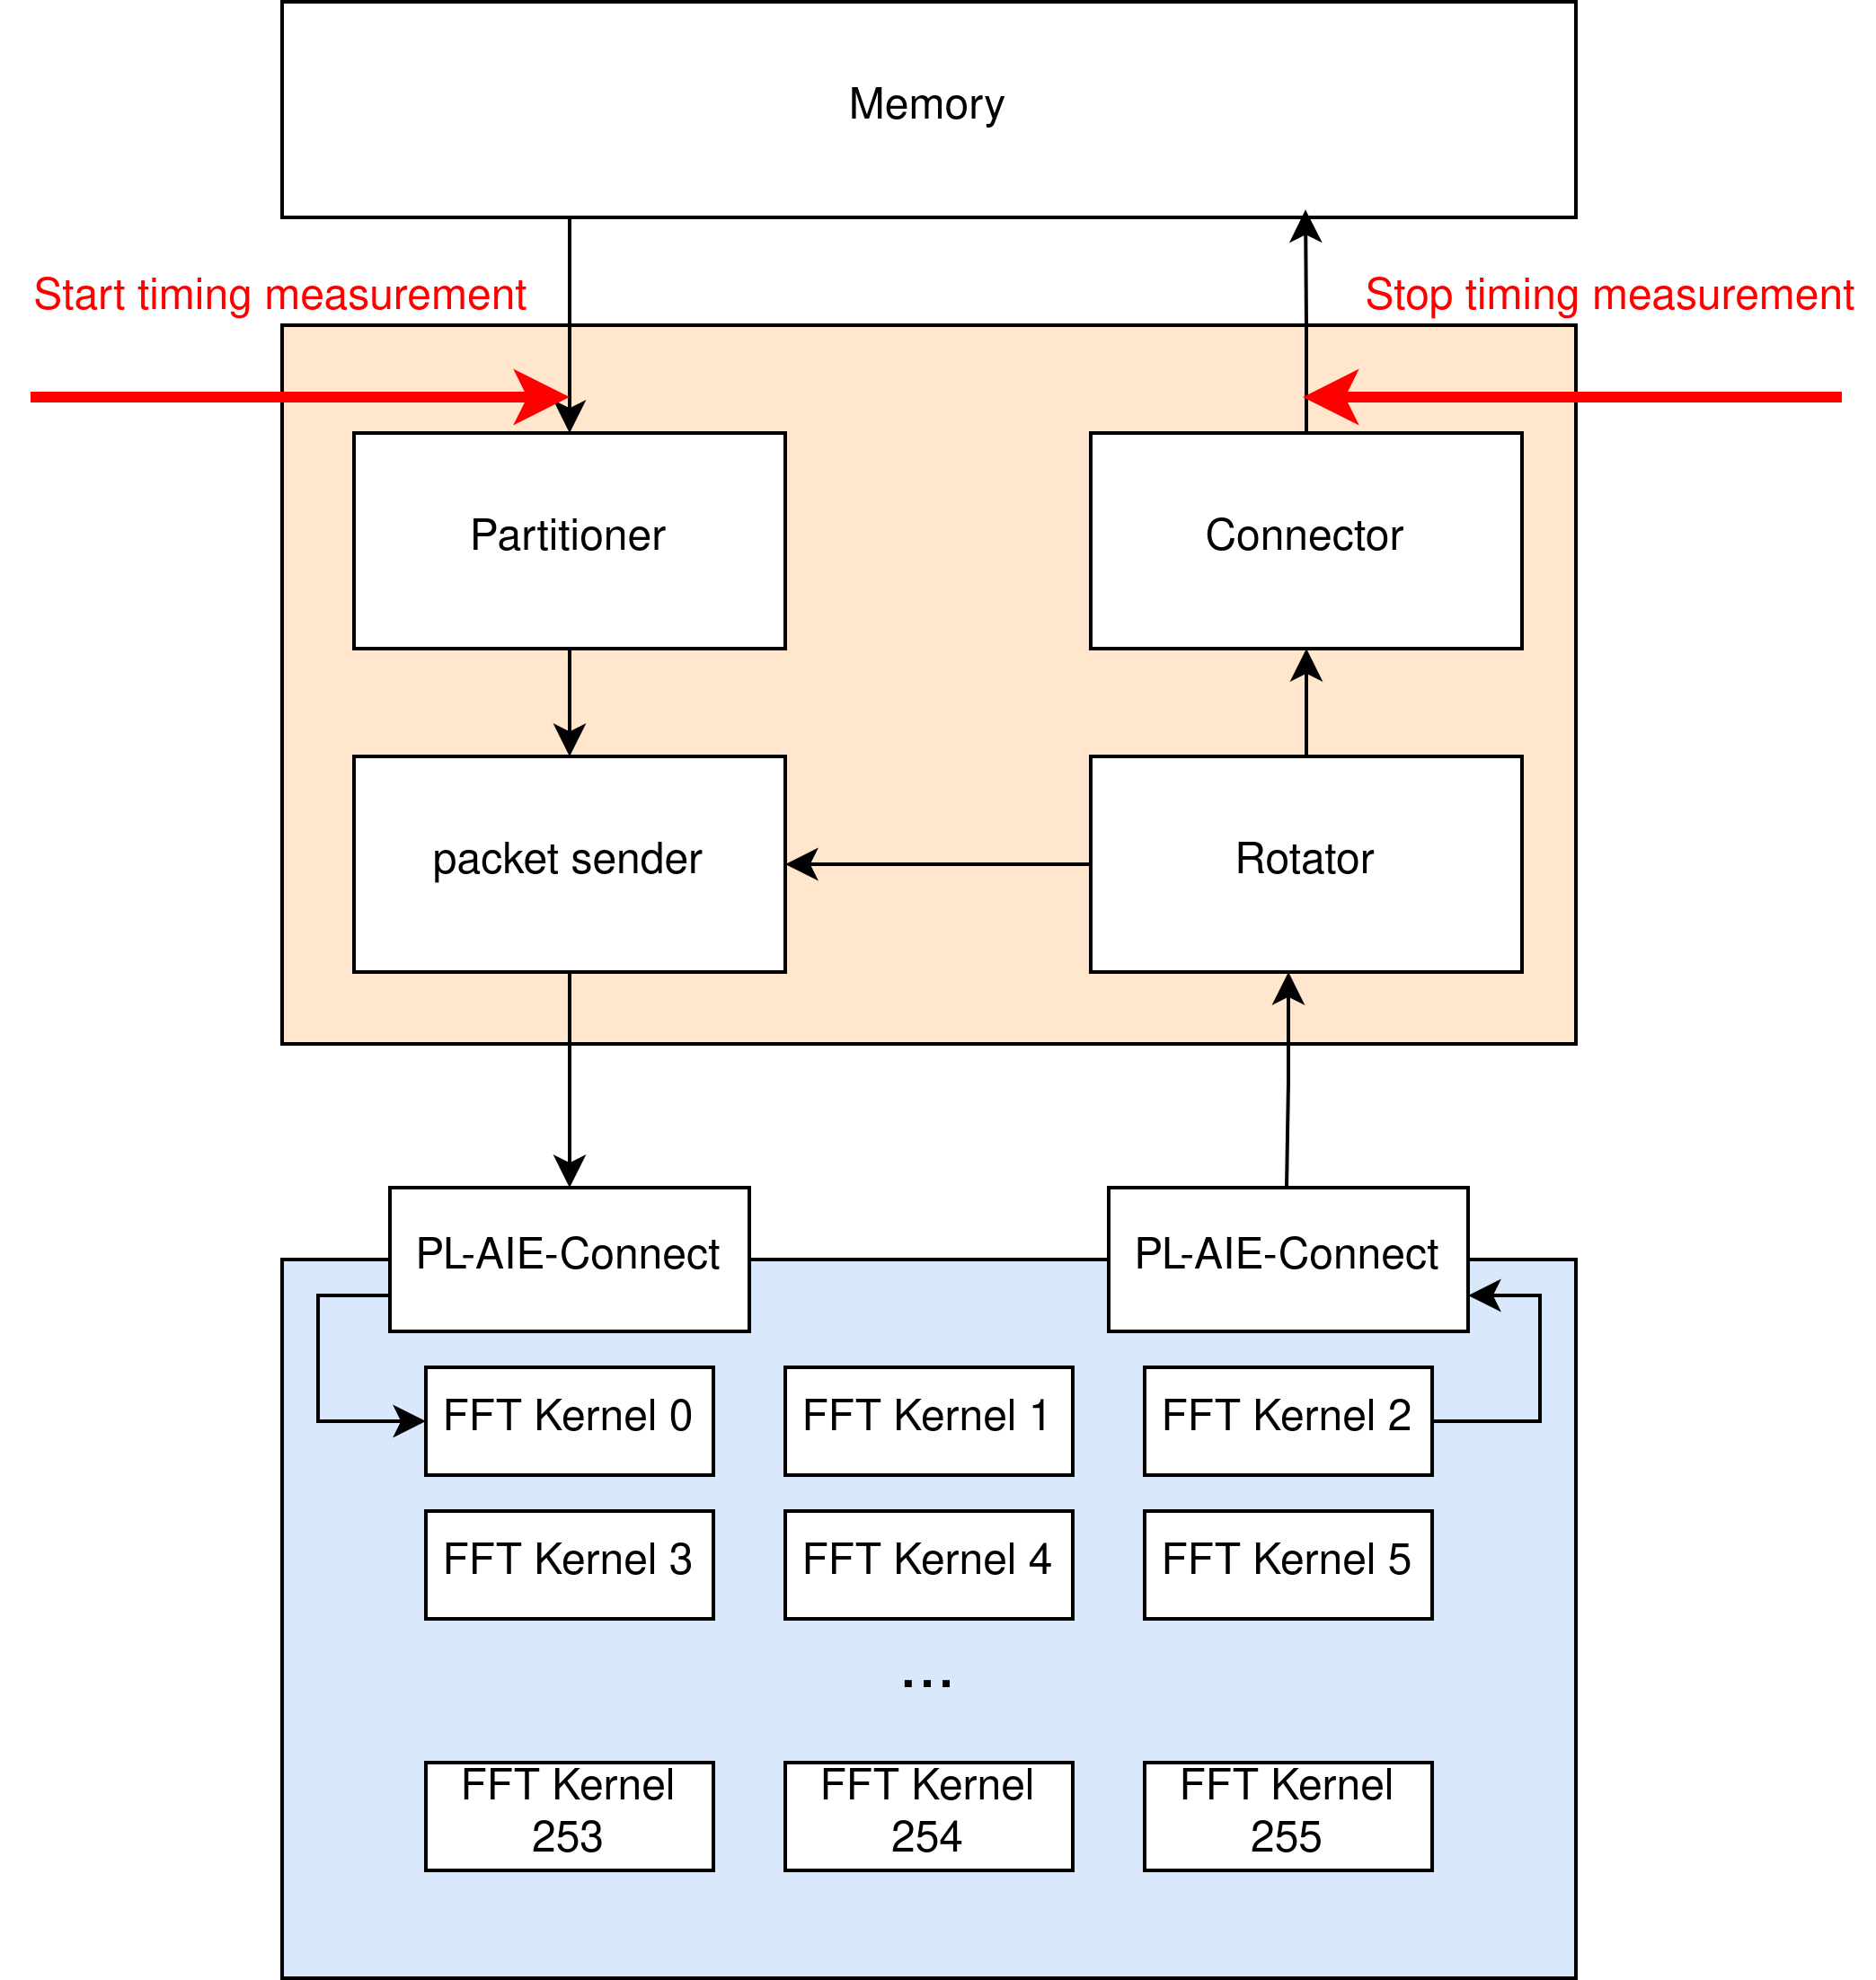
\includegraphics[width=0.6\textwidth]{images/timing.png}
    \captionsetup{justification=centering}
    \caption{Design with arrows which denotes the start and endpoint of the measurement}
    \label{fig:timing}
\end{figure}

Before presenting the results, I will briefly introduce the design choices under comparison. One of these choices is the streaming configuration of the AI Engines. There are two ways to implement streaming: the first is by reading each element from a stream and saving it to local memory, and the second is by allowing the stream to be automatically written to a predefined buffer, which is the approach used in the current design as described in section \ref{sec:aie_im}. Another important design aspect is the use of vector instructions for multiplications and additions, which could alternatively be implemented more simply on the scalar unit of the AI Engine core. Additionally, a key feature of the proposed design is the use of lookup tables for precomputed factors, so a version without this optimization will also be compared. The design further incorporates specialized load instructions for the vector units, and their impact on overall performance is also evaluated. Lastly, a comparison is made with the current complete prototype.

\section{Benchmark results}
Figure \ref{fig:plot1} illustrates the runtime performance for all test cases. To evaluate the precision of the proposed method, the root mean square error (RMSE) is also presented, with a defined threshold of -60 dB indicated by a red dotted line which was established as an acceptable error by Jensen et al. \cite{jens}. A green line at the end of the graph marks the real-time target for the algorithm. The aforementioned optimizations are applied incrementally. This means all improvements of the previous optimization step are carried over to the next which results in a ascending order of all steps in the performance diagram. In the bottom left, the naive implementation is shown, which displays a significant gap to the first optimization step. This gap is so substantial that part of the x-axis is truncated. This difference arises because the naive implementation processes each incoming stream element individually instead of buffering all elements at once. This method requires a memory instruction for each element, which not only increases the processing time per kernel but also introduces back pressure on the stream, as the stream processing time increases. This delay propagates through the entire array, resulting in a significant performance improvement when data is streamed directly into memory.\par
%TODO add plot from interime defense but with the final vector opt in the end; change the naming scheme according to this paragraph

\begin{figure}[h]
    \centering
    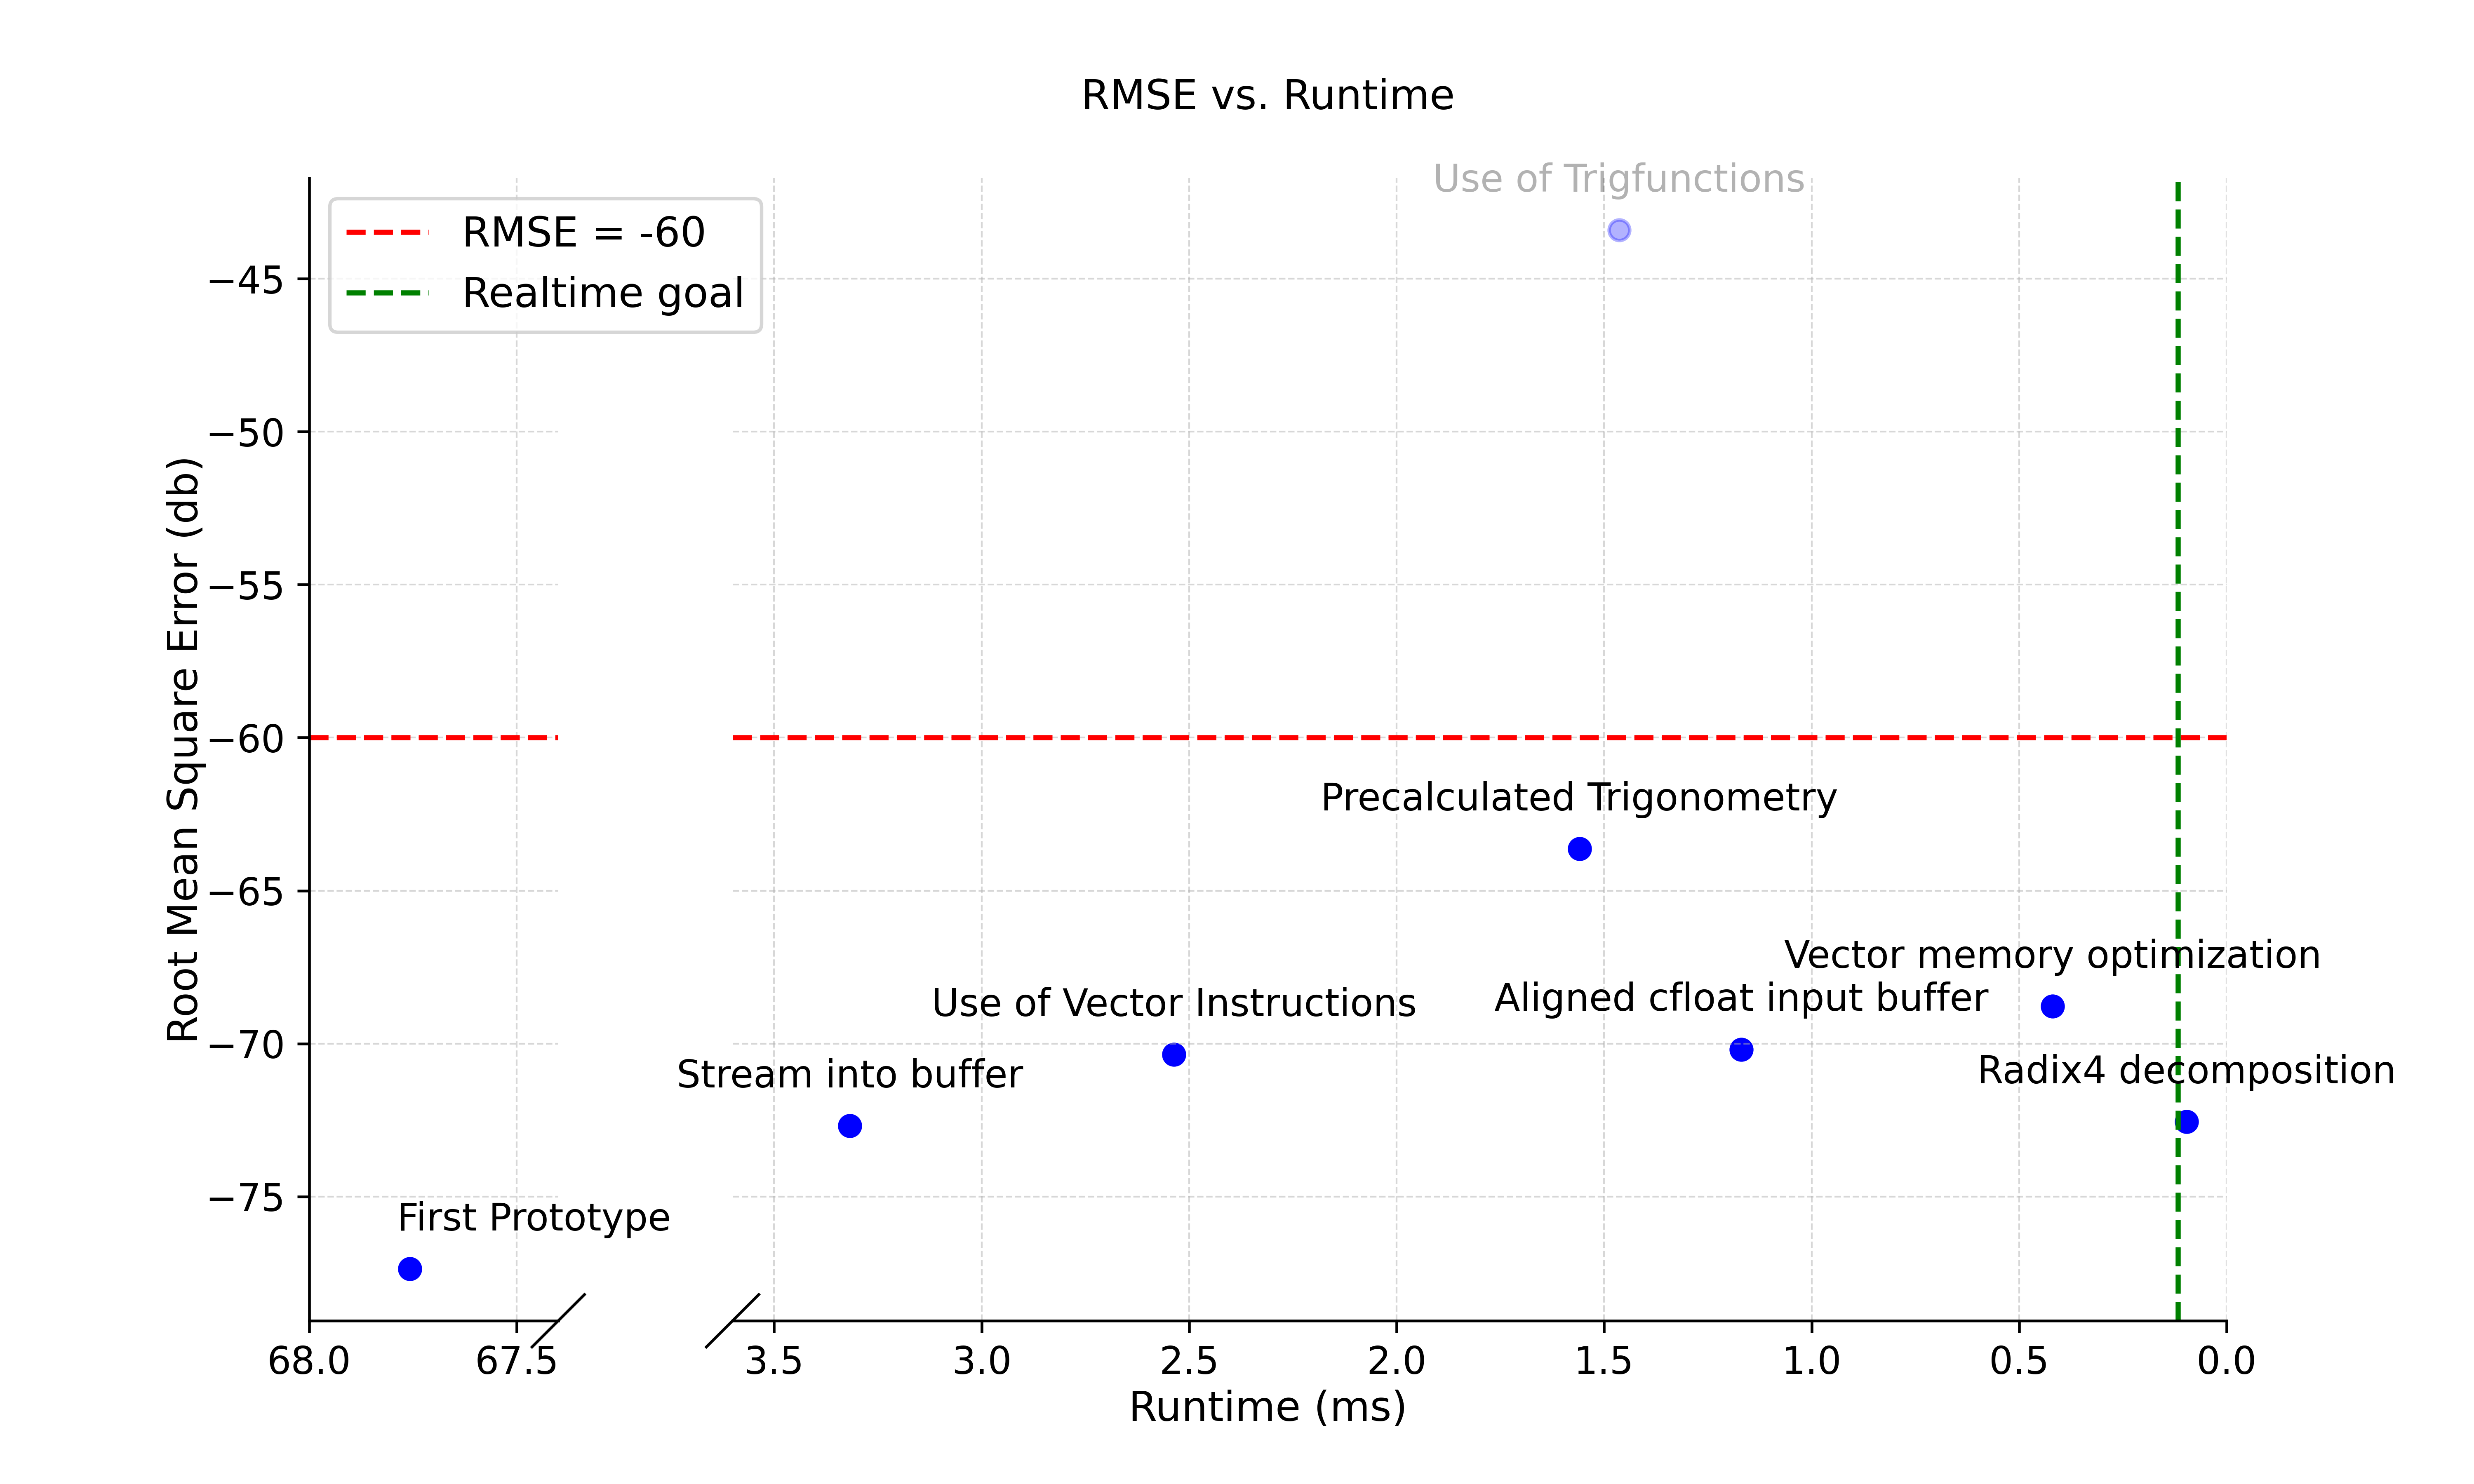
\includegraphics[width=0.9\textwidth]{images/simple_plot.png}
    \captionsetup{justification=centering}
    \caption{Various optimization steps with smaller prototype}
        Multiple iterative optimization steps in dependence from the root mean square error and the runtime. A break in the x-axis highlights the range of the runtime. The goal for realtime (green) and the maximum threshold for an error (red) are shown as dotted lines. 
    \label{fig:plot1}
\end{figure}

Figure \ref{fig:plot2} provides a different angle of the results, illustrating the different optimization steps based on the number of transformers that can be computed per second. The real-time target is again indicated by a green dotted line, assuming that 256 \ac{fft}s need to be completed within a 30 ms time frame, which equates to a real-time threshold of 8,524 \ac{fft}s per second. This representation highlights the significant performance increase achieved by utilizing the vector unit compared to all other optimizations.\par 
%TODO add throughput graph here and write paragraph about it

\begin{figure}[h]
    \centering
    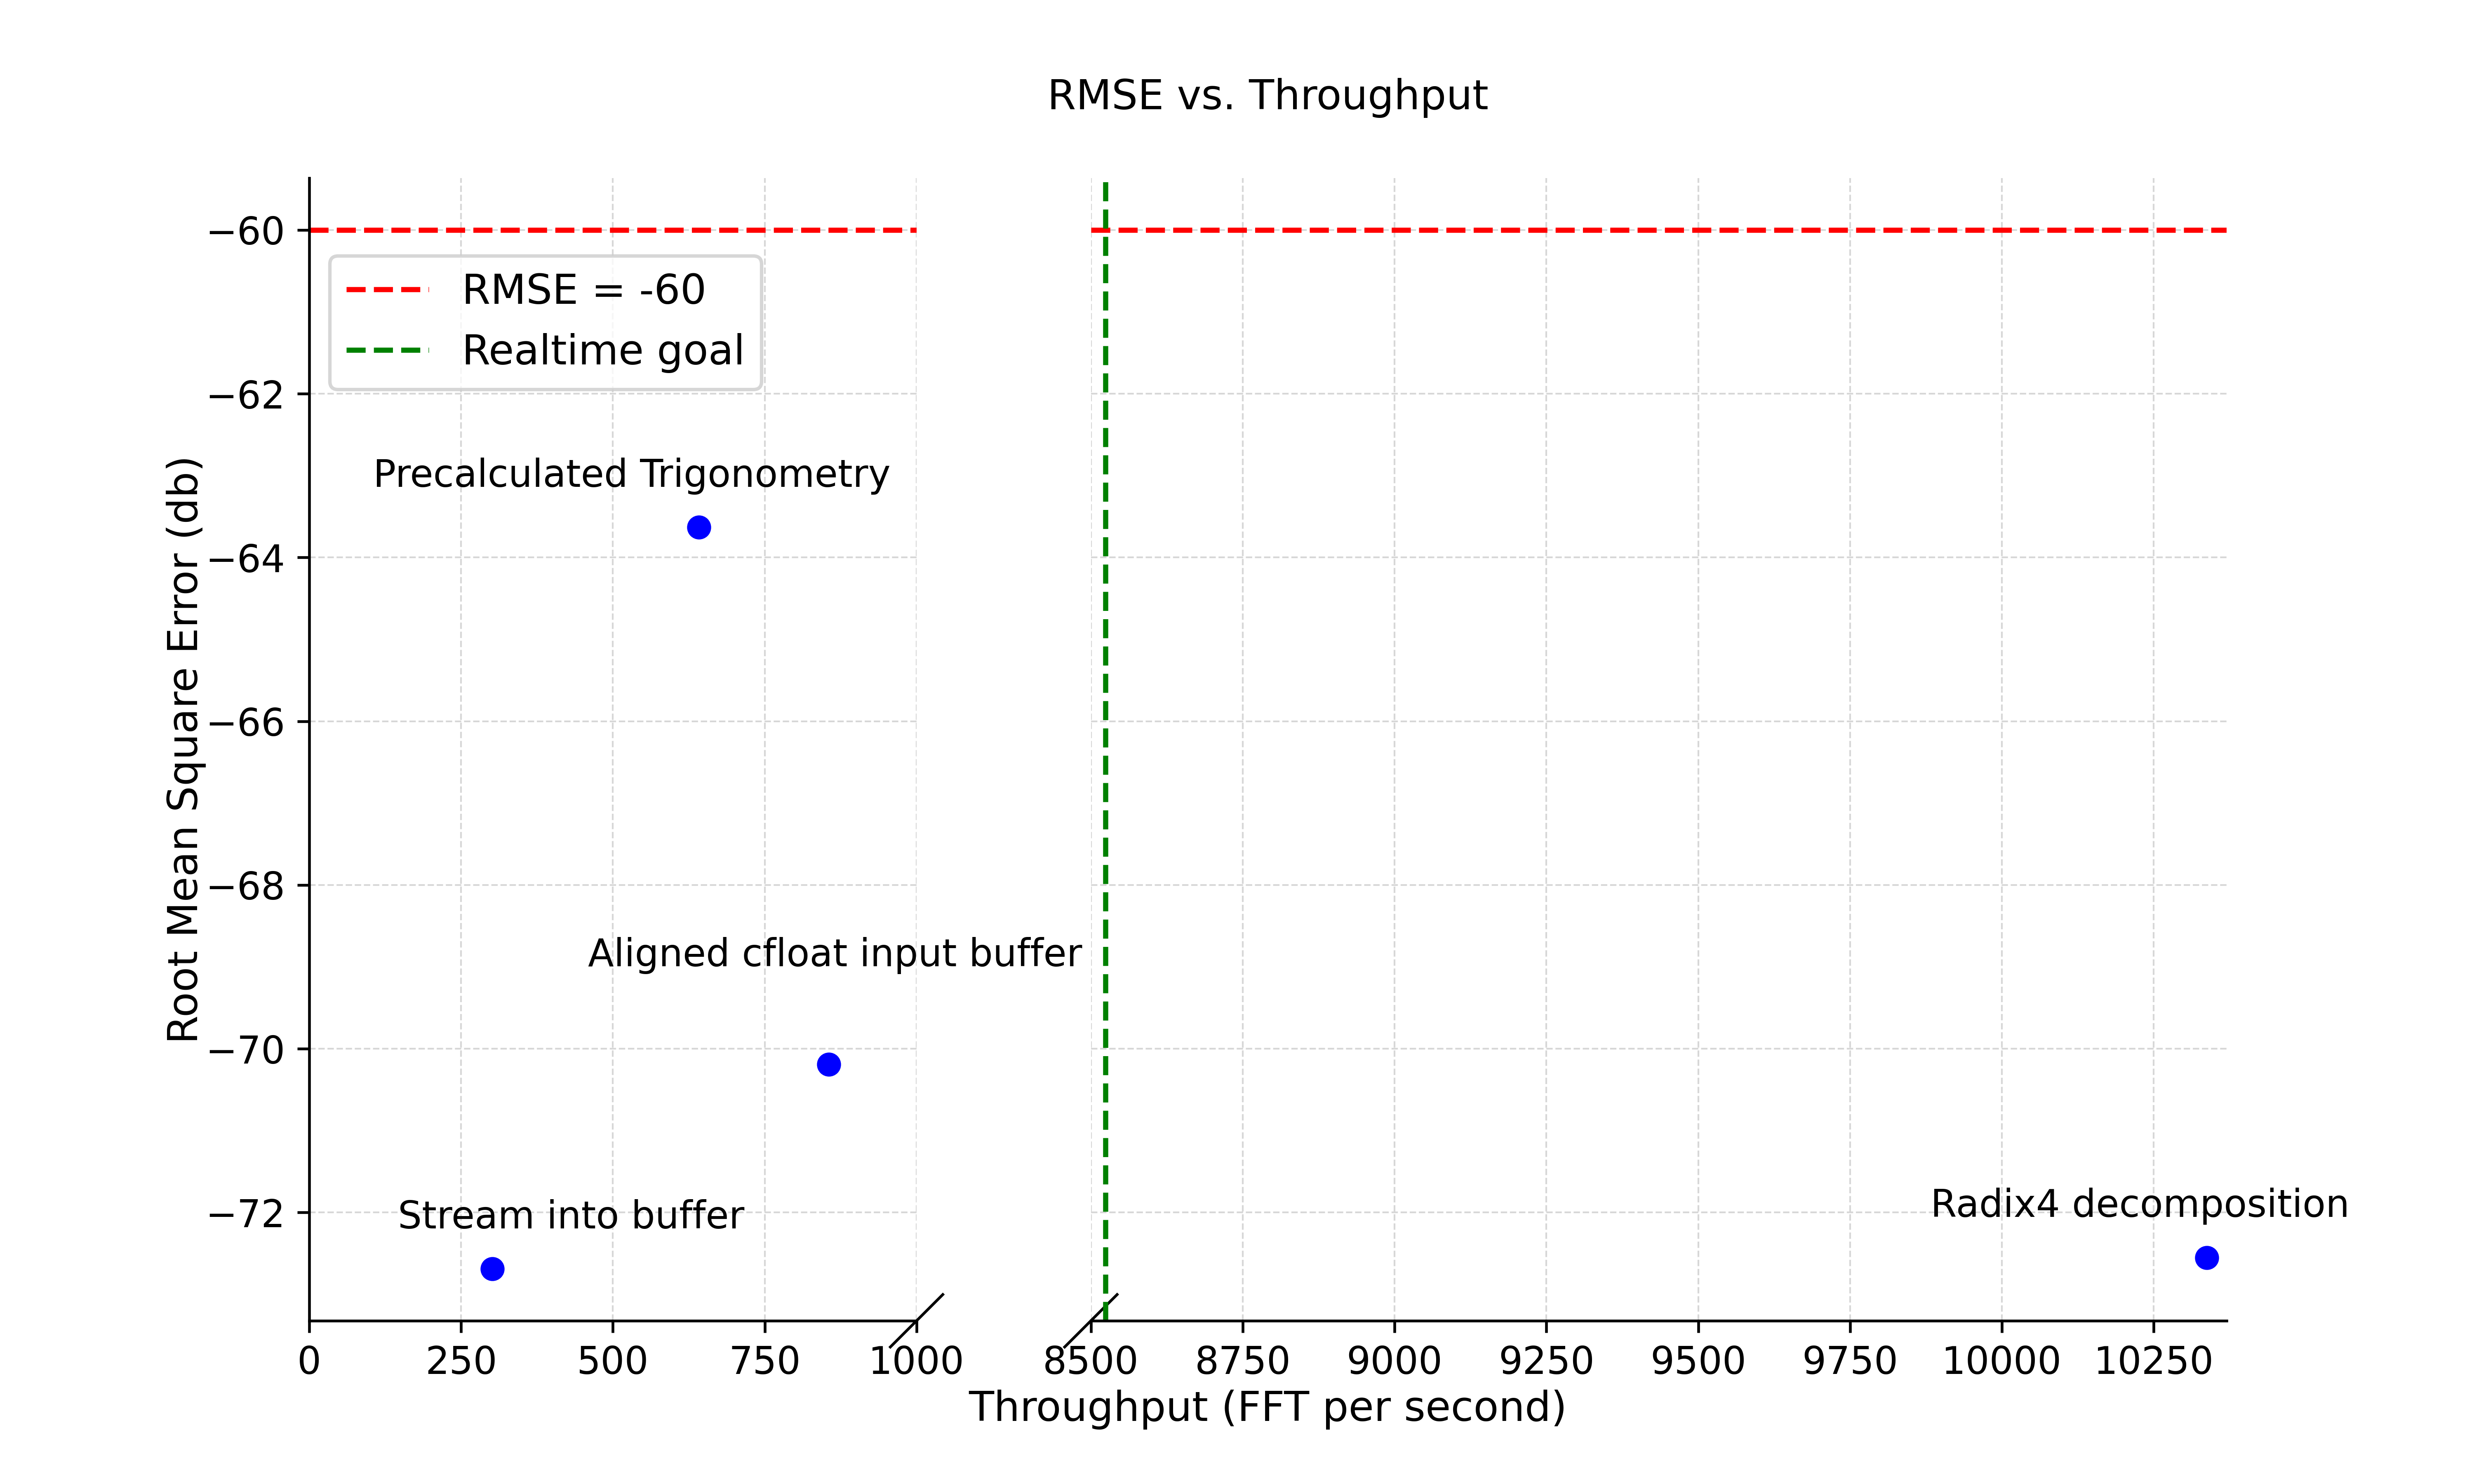
\includegraphics[width=0.9\textwidth]{images/throughput_plot.png}
    \captionsetup{justification=centering}
    \caption{Throughput of selected datapoints}
        A selection of iterative optimization steps in dependence from the error and the throughput. Through a break in the x-axis the huge difference between the optimization steps is highlighted.
    \label{fig:plot2}
\end{figure}

Another noteworthy aspect in this figure is the substantial difference in precision between using lookup tables and Xilinx-specific functions that calculate values at runtime. This discrepancy can be attributed to differences in the floating-point calculation units on the Versal platform versus the x86 processor, where values were precomputed. As shown, the precision of this method is still considerably lower than that of other optimizations and only improves when the lookup table and all other buffers are page-aligned. An analysis of the function trace revealed that this precision loss was due to a rounding function that was triggered each time a write-back occurred to a non-aligned memory location. By aligning the buffers, this precision loss was prevented. A beneficial side effect of this alignment was a reduction in runtime, as it enabled the use of faster memory access functions that operate only with aligned buffers, as described in section \ref{sec:aie_im}. The optimization using the proposed vector implementation ultimately enabled the algorithm to meet real-time requirements by reducing runtime below the real-time threshold.
%TODO add comparison in runtime between last optimization step and scale up to 262144 points

\begin{figure}[h!]
    \centering
    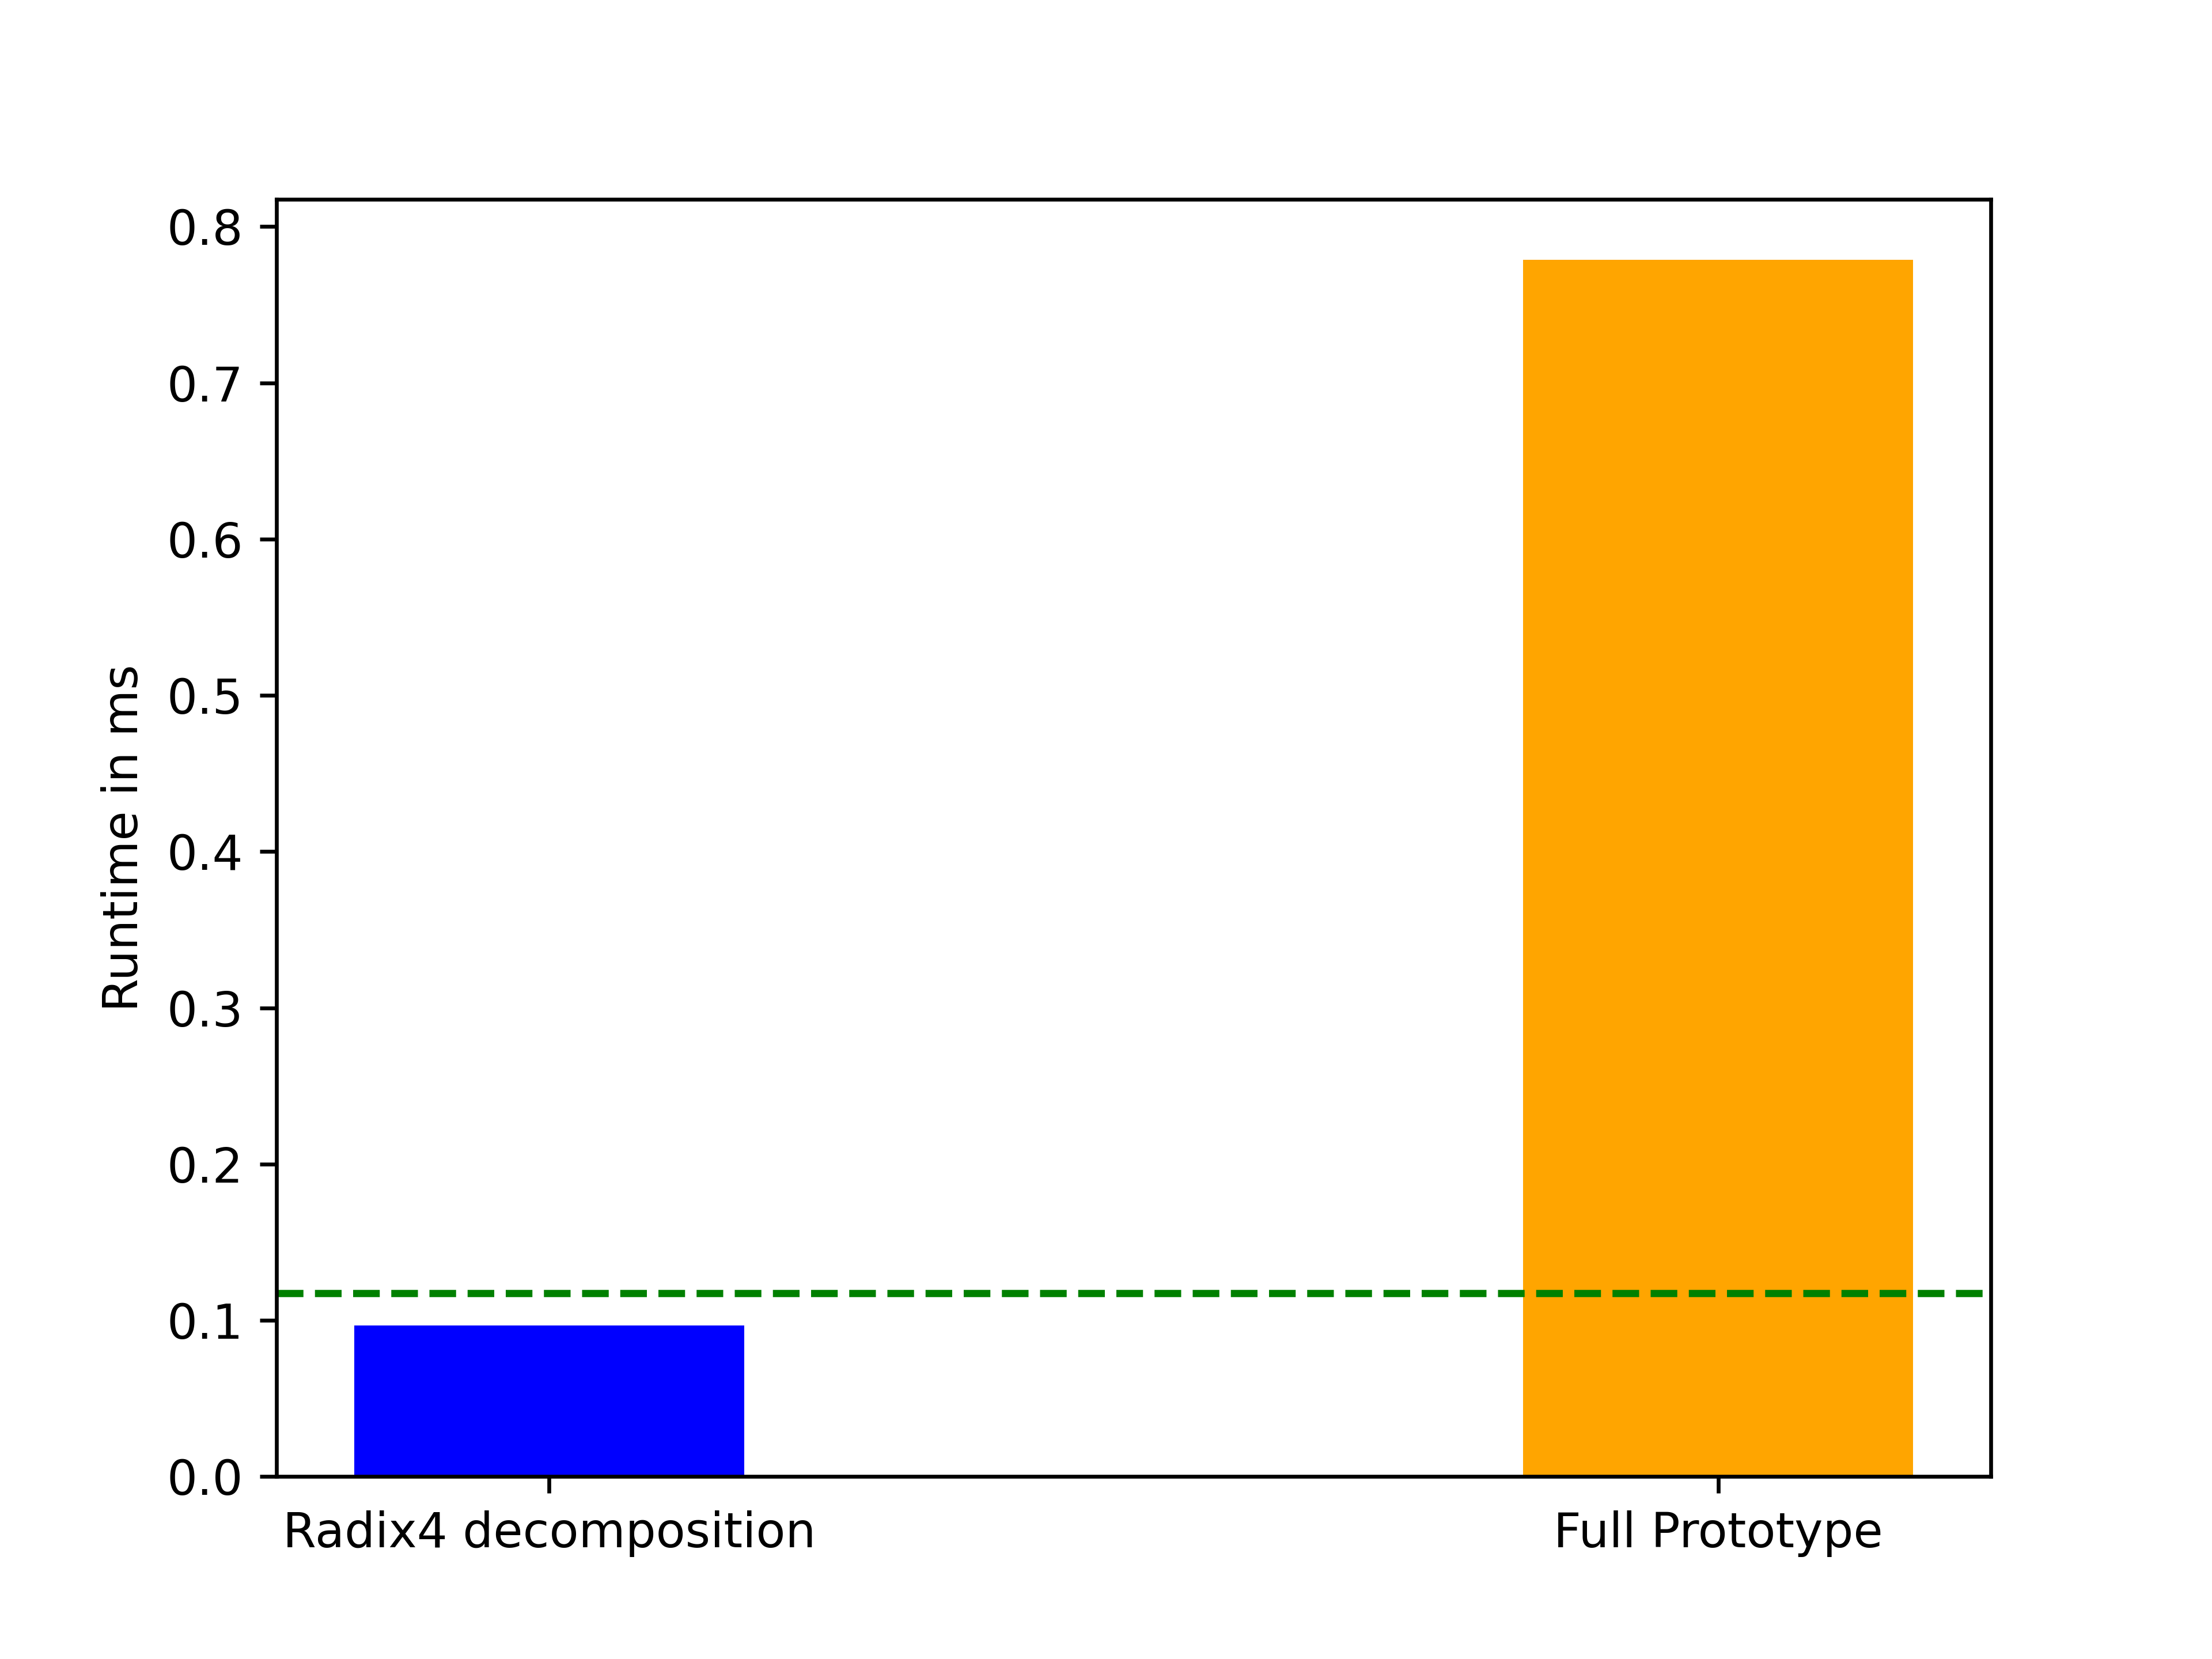
\includegraphics[width=0.6\linewidth]{images/bar_chart.png}
    \captionsetup{justification=centering}
    \caption{Comparison between the smaller and the larger prototype}
        This plot highlight the difference between a smaller prototype and the full $2^{18}$ prototype regarding runtime.
    \label{fig:last_stage}
\end{figure}
    
Figure \ref{fig:last_stage} presents a comparison between tests of a 32,768-point \ac{fft} and a $2^{18}$-point \ac{fft} using the proposed design which where both run on the previous described setup. It is evident that the larger \ac{fft} does not meet real-time requirements. To understand the source of this discrepancy, a closer examination of each component’s runtime is necessary. Figure \ref{fig:part_comp} breaks down the algorithm’s components and shows their respective runtimes, divided between the \ac{pl} and AI Engines kernels. The calculation time for the first stage exhibits a linear increase, which is expected, as the 1,024-point kernel in the $2^{18}$-point \ac{fft} uses four 256-point \ac{fft}s. Consequently, its runtime is approximately four times longer. The actual runtime is slightly higher due to additional memory management overhead and phase rotation after each 256-point \ac{fft}. The same pattern holds for the second stage kernel, which also uses four 256-point \ac{fft}s. Since this stage lacks phase rotation, its runtime aligns more closely to four times that of the smaller kernel. The noticeable gap between the second stage of the larger and smaller prototypes arises from the difference in second-stage kernel sizes, which is 128 points for the smaller prototype.\par

\begin{figure}[h]
    \centering
    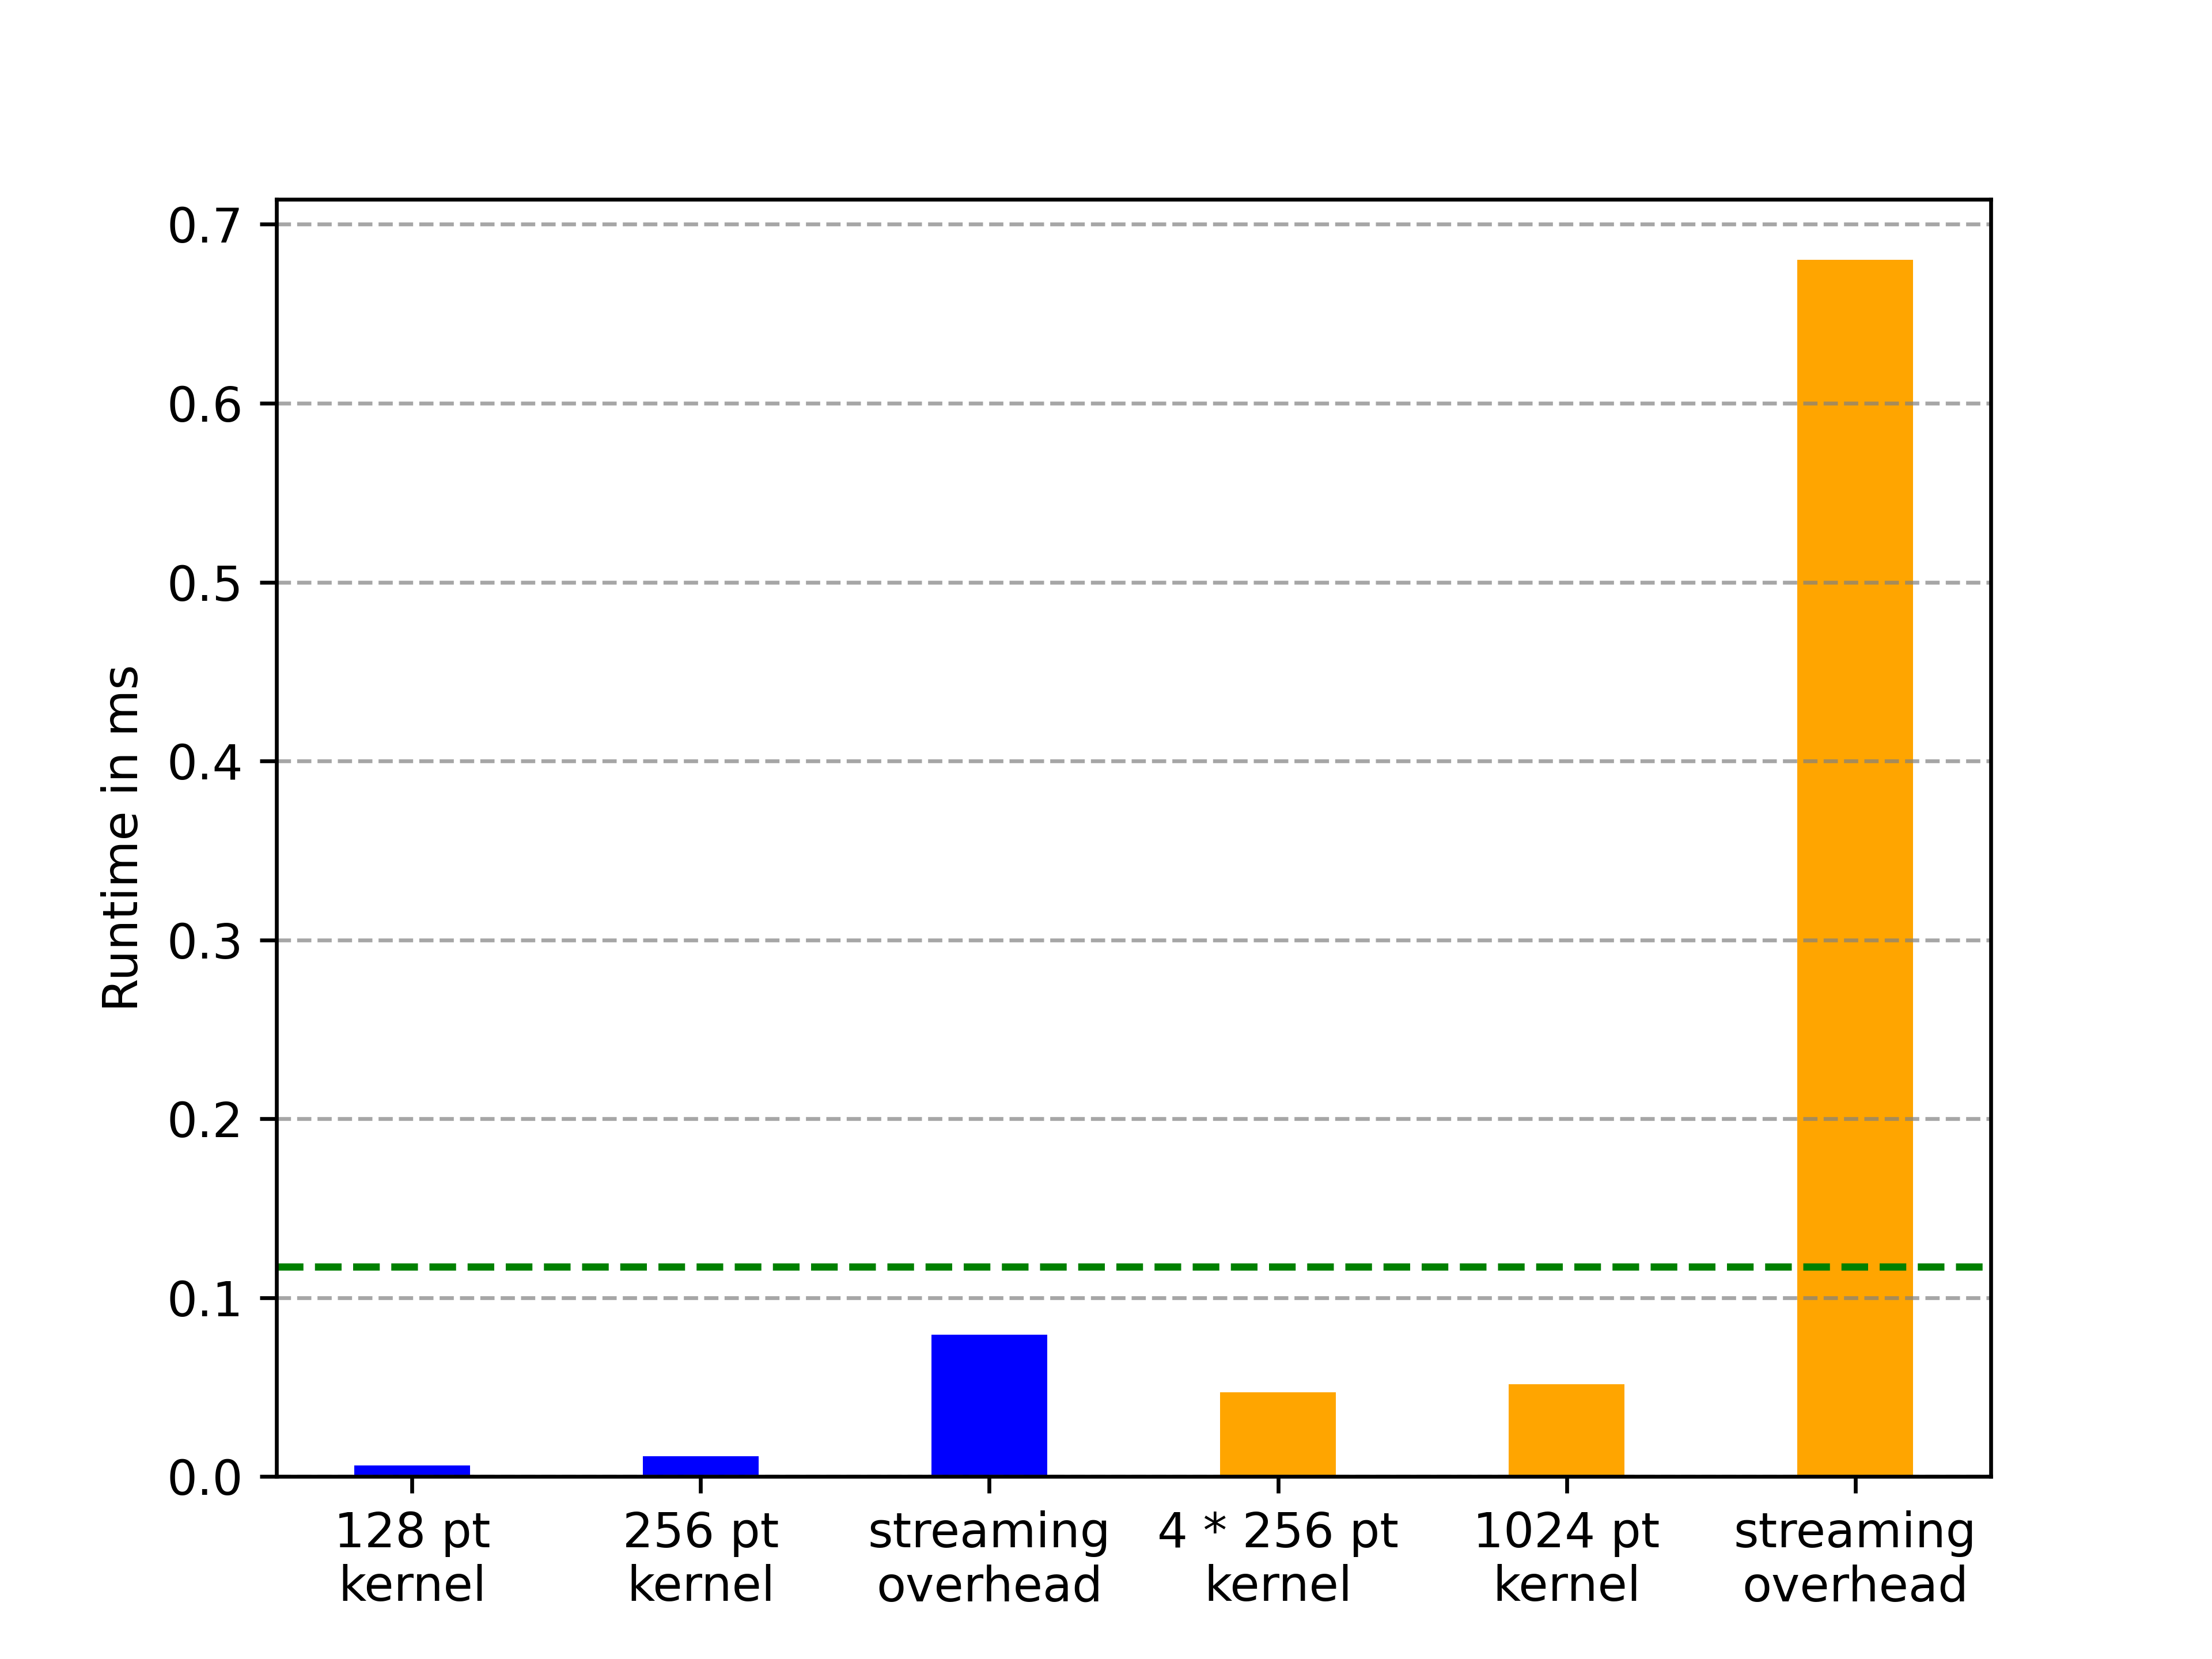
\includegraphics[width=0.6\linewidth]{images/part_comp.png}
    \captionsetup{justification=centering}
    \caption{Comparison between different stages of the algorithm}
        By splitting both, the smaller and the larger prototype, into there specific parts during runtime measurements the significant overhead of the data streaming is highlighted.
    \label{fig:part_comp}
\end{figure}

However, the most critical finding in this analysis is the time spent on streaming within the \ac{pl}. While the calculation time remains well below the real-time threshold, the interval between the first and second stages of the algorithm exceeds this limit by nearly sixfold. Several factors contribute to this issue. One is the clock frequency difference: the \ac{pl} runs at 200 MHz, whereas the AI Engines operates at 1250 MHz, leading to increased synchronization overhead between these hardware layers. This frequency mismatch also reduces the number of operations executable within a given timeframe. Additionally, the simple design of the \ac{pl}, coupled with a high-level synthesis approach where much of the implementation relies on compiler-generated code \cite{huang_survey_2020}, can result in significant underutilization of available resources.
%TODO add figure with time spend at which part of the FFT
\chapter{Summary and Outlook}\label{ch:sum}

\section{Summary}\label{sec:conclusion}
In this thesis, I developed an algorithm for computing large \ac{fft}s on a \ac{soc} platform, addressing the specific challenges of medical ultrasound imaging. The choice of platform, the Xilinx Versal VCK190, with its specialized AI accelerator processors, reflected the broader goal of advancing mobile, real-time imaging solutions. Existing \ac{fft} implementations, whether tailored for this chip or for \ac{fpga}s more broadly, were evaluated but found insufficient for the stringent real-time requirements of ultrasound imaging. This shortfall necessitated the development of a custom algorithm designed to leverage the chip's AI accelerators while maintaining compatibility with a mobile platform.\par
The proposed algorithm, built with scalability and efficiency in mind, incorporates a streaming layer in the \ac{pl} to maximize data throughput. Benchmarking revealed that while the AI accelerators were capable of handling the computational demands, the streaming layer accounted for approximately 80\% of the runtime, preventing the system from achieving full real-time performance. Nonetheless, these results underscore the potential for optimized hardware-software integration to meet the demands of high-performance imaging.\par
While the immediate application of this work lies in medical ultrasound imaging, the implications of enhancing Fourier transformation algorithms extend far beyond. As discussed in the introduction, efficient \ac{fft} computations are crucial in fields such as radar imaging and mobile communications, where rapid frequency-domain processing underpins critical applications. By demonstrating the feasibility of high-performance \ac{fft} computation on a constrained SoC platform, this study lays the groundwork for advancements across these domains.\par
Future research could focus on overcoming the identified bottlenecks by manually optimizing the streaming layer using Verilog or VHDL or exploring the trade-offs of reduced data precision. Additionally, given the rapid evolution of AI accelerator technology, alternative chip architectures could further unlock real-time performance and scalability. These pathways offer exciting opportunities not only for improving ultrasound imaging but also for enhancing computational techniques in related fields.\par
In conclusion, this work represents a significant step toward realizing the vision outlined in the beginning: portable, high-performance imaging systems capable of transforming both clinical and non-clinical applications. While challenges remain, the foundation established here highlights the potential for real-time, frequency-domain processing to redefine the capabilities of imaging technologies.

\section{Outlook}\label{sec:future}
The previous chapter demonstrated promising results for utilizing a large real-time \ac{fft}. However, as shown by these results, the threshold for a fully real-time capable design and implementation of 8,524 FFTs per seconds has not yet been achieved. One of the primary contributing factors is the data streaming within the \ac{pl}. Since this was not the main focus of this work, a potential first step in further optimization could be a deeper investigation of streaming methods specifically suited to this purpose. The \ac{pl} is similar to a standard \ac{fpga}, which raises the question of whether streaming methods used in network applications, which also heavily depend on \ac{fpga}s, could be adapted here. In high-capacity network backbones, data streaming rates in the hundred gigabyte per second range are achievable \cite{jankovic_high-capacity_2020}. In comparison, the real-time target for this project requires a streaming rate of approximately 29 gigabytes per second, assuming the use of 64-bit complex floating-point values.\par
Another promising avenue for exploration is the potential reduction of resolution of the used data. Lowering the resolution could not only improve the streaming efficiency of the \ac{pl} but also expand the design space for the AI Engines. The Xilinx intrinsic functions, for instance, support data types down to 8 bits, allowing multiple values to be processed simultaneously in vector registers \cite{henry_leveraging_2019}. This change could also alleviate some of the memory constraints during streaming within the AI Engine array. A thorough analysis of precision requirements would be essential to determine whether this approach would indeed be advantageous. Alternatively, precision adjustments could focus not on the working data itself but on the precomputed values, which could help mitigate memory constraints without significantly impacting overall precision.\par
The exploration of precision leads to a broader question: the analysis of the entire system and the effect of precision on subsequent stages in the image generation pipeline. This would involve application-level testing of the algorithm through repeated or continuous execution. Such an approach would address some limitations of the test pipeline used in this study, which primarily assessed runtime and correctness based on a single algorithmic execution.\par
Another direction for future research could be experimenting with different hardware. The algorithm presented here largely employs a target offloading approach, which might also benefit from application to other hardware platforms. Examining the potential of accelerators may offer additional advantages, especially considering that the current design utilizes AI Engines in an accelerator-like capacity. Furthermore, investigating larger ACAP devices, which offer not only increased computational resources but also expanded memory capacity, could be advantageous given that memory is a key limiting factor in this design.

%\appendix

\listoffigures
\listoftables



%\begin{description}
%\end{description}

\bibliographystyle{acm}
\bibliography{own}

\end{document}

